%%%%%%%%%%%%%%%%%%%%%%%%%%%%%%%%%%%%%%%%%
% The Legrand Orange Book
% LaTeX Template
% Version 3.1 (February 18, 2022)
%
% This template originates from:
% https://www.LaTeXTemplates.com
%
% Authors:
% Vel (vel@latextemplates.com)
% Mathias Legrand (legrand.mathias@gmail.com)
%
% License:
% CC BY-NC-SA 4.0 (https://creativecommons.org/licenses/by-nc-sa/4.0/)
%
% Compiling this template:
% This template uses biber for its bibliography and makeindex for its index.
% When you first open the template, compile it from the command line with the 
% commands below to make sure your LaTeX distribution is configured correctly:
%
% 1) pdflatex main
% 2) makeindex main.idx -s indexstyle.ist
% 3) biber main
% 4) pdflatex main x 2
%
% After this, when you wish to update the bibliography/index use the appropriate
% command above and make sure to compile with pdflatex several times 
% afterwards to propagate your changes to the document.
%
%%%%%%%%%%%%%%%%%%%%%%%%%%%%%%%%%%%%%%%%%

%----------------------------------------------------------------------------------------
%	PACKAGES AND OTHER DOCUMENT CONFIGURATIONS
%----------------------------------------------------------------------------------------

\documentclass[
	UTF-8,
	11pt, % Default font size, select one of 10pt, 11pt or 12pt
	% fleqn, % Left align equations
	a4paper, % Paper size, use either 'a4paper' for A4 size or 'letterpaper' for US letter size
	%oneside, % Uncomment for oneside mode, this doesn't start new chapters and parts on odd pages (adding an empty page if required), this mode is more suitable if the book is to be read on a screen instead of printed
]{LegrandOrangeBook}

% Book information for PDF metadata, remove/comment this block if not required 
\hypersetup{
	pdftitle={Title}, % Title field
	pdfauthor={Author}, % Author field
	pdfsubject={Subject}, % Subject field
	pdfkeywords={Keyword1, Keyword2, ...}, % Keywords
	pdfcreator={LaTeX}, % Content creator field
}

\addbibresource{sample.bib} % Bibliography file

\definecolor{ocre}{RGB}{0, 0, 160} % Define the color used for highlighting throughout the book

\chapterimage{orange1.jpg} % Chapter heading image
\chapterspaceabove{6.5cm} % Default whitespace from the top of the page to the chapter title on chapter pages
\chapterspacebelow{6.75cm} % Default amount of vertical whitespace from the top margin to the start of the text on chapter pages

\setenumerate{itemsep=0.5em, topsep=0.5em, partopsep=0.25em}

%----------------------------------------------------------------------------------------

\usepackage{xeCJK}          % 中/日/韓文字處理

\usepackage{fontspec}       % OpenType/TrueType字體支持

\usepackage{unicode-math}   % Unicode數學字體支持

\usepackage{tikz}
\usetikzlibrary{decorations.pathreplacing} 
\usetikzlibrary{shapes, positioning, arrows.meta, fit, backgrounds,calc}

\setmainfont{Latin Modern Math}[BoldFont = Latin Modern Math,
  BoldFeatures = {FakeBold=2} ] 
  % 英文主字體
\setmathfont{TeX Gyre Termes Math} % 數學符號字體
\setmathfont{XITS Math}[
  range={\mitpi},
  Scale=1  % 調整大小以匹配主字體
]
\setmathfont{Times New Roman}[
  range={"25},
  Scale=1  % 調整大小以匹配主字體
]
\setmathfont{Times New Roman}[
  range={\sum,\prod},
  Scale=1.5  % 調整大小以匹配主字體
]
\setmathfont{Times New Roman}[
  range={\int},
  Scale=2.1  % 調整大小以匹配主字體
]
\setmathfont{Latin Modern Math}[
  range={\sqrt,\forall,\exists, 
  "2B, "2D, "3D, "2260 ,\times, \div, \pm, \cdot, \leq, \geq, \in, \notin, \subset,
    \supset, \subseteq, \supseteq, \cup, \Rightarrow, \Leftarrow,\rightarrow, \leftarrow, \Leftrightarrow ,
     \cap, \wedge, \vee, \neg,\Longleftrightarrow ,\Longrightarrow ,\longrightarrow,\Longleftarrow,\longleftarrow 
     ,\Uparrow ,\Downarrow ,\Updownarrow,\bigcap,\bigcup,\longmapsto,\mapsto,\nrightarrow,\nLeftrightarrow},
  Scale=1  % 調整大小以匹配主字體
]

	% \setCJKmainfont[AutoFakeSlant=true]{LXGW 975 HazyGo SC 300W}
    % \setCJKsansfont[AutoFakeSlant=true]{Source Han Sans CN VF}
    % \setCJKmonofont[AutoFakeSlant=true]{Source Han Sans CN VF}

%----------------------------------------------------------------------------------------

\begin{document}

\xeCJKsetup{
    CJKglue={\hskip 0.5pt plus 0.35\baselineskip},
    CJKecglue={\hspace{2pt}},
    CJKmath=true
    }
\setlength{\mathsurround}{0.25em}

%----------------------------------------------------------------------------------------
%	TITLE PAGE
%----------------------------------------------------------------------------------------

\titlepage % Output the title page
	{
\includegraphics[width=\paperwidth]{A.jpg}} % Code to output the background image, which should be the same dimensions as the paper to fill the page entirely; leave empty for no background image
	{ % Title(s) and author(s)
		\centering\sffamily % Font styling
		{\Huge\bfseries Mathematical Analysis and Real Analysis \par} % Book title
		\vspace{8pt} % Vertical whitespace
		{\large Key points of proofs for Undergrade Students \\ Vol.1 \par} % Subtitle
		\vspace{12pt} % Vertical whitespace
		{\LARGE Xuless \par} % Subtitle
		{\large Department of Mathematics \par} % Subtitle
        \vspace{12pt}
        {\large ***Helpful for \textbf{MATH 1023,1024,2033,3033}*** \par} % Subtitle
		\vspace{24pt} % Vertical whitespace
		{\huge\bfseries Hong Kong University of Science and Technology \par} % Author name
	}

%----------------------------------------------------------------------------------------
%	COPYRIGHT PAGE
%----------------------------------------------------------------------------------------

\thispagestyle{empty} % Suppress headers and footers on this page

~\vfill % Push the text down to the bottom of the page

\noindent Copyright \copyright\ 2022 Goro Akechi\\ % Copyright notice

\noindent \textsc{Published by Publisher}\\ % Publisher

\noindent \textsc{\href{https://www.latextemplates.com/template/legrand-orange-book}{book-website.com}}\\ % URL

\noindent Licensed under the Creative Commons Attribution-NonCommercial 4.0 License (the ``License''). You may not use this file except in compliance with the License. You may obtain a copy of the License at \url{https://creativecommons.org/licenses/by-nc-sa/4.0}. Unless required by applicable law or agreed to in writing, software distributed under the License is distributed on an \textsc{``as is'' basis, without warranties or conditions of any kind}, either express or implied. See the License for the specific language governing permissions and limitations under the License.\\ % License information, replace this with your own license (if any)

\noindent \textit{First printing, March 2022} % Printing/edition date

\newpage

%----------------------------------------------------------------------------------------
%	TABLE OF PREFACE
%----------------------------------------------------------------------------------------

\thispagestyle{empty} % Suppress headers and footers on this page

\begin{center}
    \textbf{\LARGE Preface:}
\end{center}

This book is the study notes of HKUST mathematics courses. Applicable to 
series of courses of \textbf{MATH 2033, MATH 3033} or \textbf{MATH 1023, MATH 1024}. \\

Moreover, before use this notes, you may hold some basic knowledge of \textbf{MATH 1013, MATH 1014,MATH 2001} and 
\textbf{MATH 2121}. This book does not review prerequisite courses for applicable courses.\\

\begin{center}
    \textbf{\LARGE 序言:}
\end{center}

本书是香港科技大学数学课程的学习笔记。适用于 
\textbf{MATH 2033, MATH 3033} 或 \textbf{MATH 1023, MATH 1024} 系列课程。 \\

此外，在使用本笔记之前，您可能已经掌握了 \textbf{MATH 1013, MATH 1014,MATH 2001} 以及 
\textbf{MATH 2121} 的一些基本知识。本书不会对适用课程的前置课程进行复习。\\

\begin{quote}
    This book draws on the following:
    \begin{enumerate}
        \item Mathematical analysis $2^{\text{nd}}$ Edit  [Tom.M.Apostol]
        \item Principle of mathematical analysis $3^\text{{rd}}$ Edit [Walter Rudin]
        \item The note of MATH 2033 [Dr. Ku, Yin Bon]
        \item The note of MATH 3033 [Dr. Ku, Yin Bon]
        \item The note of MATH 2043 [Prof . Min Yan]
    \end{enumerate}

\end{quote}




%----------------------------------------------------------------------------------------
%	TABLE OF CONTENTS
%----------------------------------------------------------------------------------------

\pagestyle{empty} % Disable headers and footers for the following pages

\tableofcontents % Output the table of contents

% \listoffigures % Output the list of figures, comment or remove this command if not required

% \listoftables % Output the list of tables, comment or remove this command if not required

\pagestyle{fancy} % Enable default headers and footers again

\cleardoublepage % Start the following content on a new page

%----------------------------------------------------------------------------------------
%	PART
%----------------------------------------------------------------------------------------

\part{Part I: Mathematical Analysis }

%----------------------------------------------------------------------------------------
%	SECTIONING EXAMPLES CHAPTER
%----------------------------------------------------------------------------------------

\chapterimage{orange2.jpg} % Chapter heading image
\chapterspaceabove{6.75cm} % Whitespace from the top of the page to the chapter title on chapter pages
\chapterspacebelow{7.25cm} % Amount of vertical whitespace from the top margin to the start of the text on chapter pages

%------------------------------------------------
\renewcommand{\setminus}{\backslash}

\chapter{Basic Concepts}

\section{Set}

\subsection{Basic definition}

\begin{definition}[Set]
	A set is a collection of objects. We use the symbol $\{ \}$ to describe the set.
	The object in a set called element or member (元素).
\end{definition}

\begin{example}
	Let $S = \{ 1,2,3,4 \}$, we say $1,2,3,4$ are elements of $S$.
\end{example}

\begin{definition}
	Suppose $S$ is a set. $x$ is an element (or a member) of $S$, if $x$ is in the set $S$, denoted by
	$$x \in S$$
	We write $x \notin S$ if $x$ is not an element of $S$.
\end{definition}

\begin{example}
	Let $S = \{ a,b,c,d \}$, we have $a \in S,\ b\in S, \cdots$, but $e \notin S$.
\end{example}


\begin{definition}
	Any set can be writs as the follow form:
	$$\{ \text{Form of object} \ |\ \text{statement to describe the object} \}$$
\end{definition}

\begin{remark}
	We often use $:$ to replace $|$, like: $\{ \text{Form of object} \ :\ \text{statement to describe the object} \}$.\\
	(“$:$” 与 “$|$” 可以互相混用，不影响表述。)
\end{remark}

\begin{example}
	The set of all nature number can be write as:
	$$
	\{ n\ |\ n\ \text{is nature number} \}
	$$
	there are same to write $\{1,2,3,4,5,6,7,\cdots\}$.
\end{example}

\newpage

\begin{definition}[Common Sets of Numbers]
The following notations are standard for describing specific sets of numbers:
\begin{itemize}[itemsep = 1em,topsep = 1ex]
    \item $\emptyset$: The \textbf{empty set} (空集), which is the unique set containing no elements.
    \item $\mathbb{N}$: The set of all \textbf{natural numbers} (自然数). Typically defined as $\mathbb{N} = \{1, 2, 3, \dots\}$.
    \item $\mathbb{Z}$: The set of all \textbf{integers} (整数). Defined as $\mathbb{Z} = \{ \dots, -2, -1, 0, 1, 2, \dots \}$.
    \item $\mathbb{Q}$: The set of all \textbf{rational numbers} (有理数). These are numbers that can be expressed as a fraction $\frac{p}{q}$ where $p, q \in \mathbb{Z}$ and $q \neq 0$.
    \item $\mathbb{R}$: The set of all \textbf{real numbers} (实数), representing points on a continuous number line.
    \item $\mathbb{C}$: The set of all \textbf{complex numbers} (复数), typically in the form $a + bi$ where $a, b \in \mathbb{R}$ and $i = \sqrt{-1}$.
\end{itemize}
\end{definition}

\begin{example}\quad
	\begin{itemize}[itemsep = 1em,topsep = 1ex]
    \item $5 \in \mathbb{N}$ (Also in $\mathbb{Z}, \mathbb{Q}, \mathbb{R}, \mathbb{C}$)
    \item $-3 \in \mathbb{Z}$ (Not in $\mathbb{N}$, but in $\mathbb{Q}, \mathbb{R}, \mathbb{C}$)
    \item $0.5 \in \mathbb{Q}$ (Not in $\mathbb{Z}$, but in $\mathbb{R}, \mathbb{C}$)
    \item $\sqrt{2} \in \mathbb{R}$ (Not in $\mathbb{Q}$, but in $\mathbb{C}$)
    \item $1+i \in \mathbb{C}$ (Not in $\mathbb{R}$)
	\end{itemize}
\end{example}

\begin{definition}[Subset]
	Given two sets $A$ and $B$,we say $A$ is a subset (子集) of $B$ if $$\forall x,\ x \in A \implies x \in B$$
	denoted by $A \subseteq B$. In
	particular, $A = B$ iff $$A \subseteq B \land B \subseteq A$$ 
	i.e. $\forall x,\ x\in A \iff x \in B$. If $A$ is a subset of $B$ but $A\neq B$, we say $A$
	is a proper subset(真子集) of $B$, denoted by $A \subset B$.
\end{definition}

\begin{remark}
	$\emptyset \subseteq A$ for all set $A$.
\end{remark}

\begin{example}
	Let $S= \left\{ n \in \mathbb{Z} \ | \ n = 2k, \forall k \in \mathbb{Z} \right\}$, there are means $n$ 
	are the even integer, so $S$ is the set of all even integer. Since take any $x \in S$, $x$ is an even integer,
	so $x$ is an integer, so $x \in \mathbb{Z}$, i.e. $x \in S \implies x \in \mathbb{Z}$ .
	We have $S \subseteq \mathbb{Z}$, and $1 \in \mathbb{Z}$ but $1 \notin S$, 
	so $x\in \mathbb{Z} \ \text{not implies} \ x \in S$, we have $S \subset \mathbb{Z}$.
\end{example}

\newpage

\subsection{Power set}

\begin{definition}[Power set]
	Given a set $S$. The power set(幂集) of $S$ is the set of all subsets of $S$, denoted by $P(S)$ or $2^S$.
\end{definition}

\begin{example}
	Suppose $S = \{1, 2, 3\}$. Then we have
	$$2^S = \{\emptyset, \{1\} , \{2\} , \{3\} , \{1, 2\} , \{2, 3\} , \{1, 3\} , \{1, 2, 3\}\}$$
	and we can prove for any set $S$, $S \in P(S)$, see the follows proposition.
\end{example}

\begin{proposition}
	For any set $S$, $S \in P(S)$.
\end{proposition}

\begin{proof}
	$P(S)$ is the set of all subset of $S$ by definition. So $S \in P(S)$ means $S$ 
	is the subset of itself (\textbf{This is the aim we want to prove}). \\

	Note that we must have
	$$S \subseteq S$$
	since $\forall x, x \in S \implies x \in S $. So $S$ is the subset of itself.
\end{proof}

\begin{remark}
	Write down the definition begin the proof is so useful.\\
	(在证明之前写下部分定义有助于证明。)
\end{remark}

Why we use the symbol $2^S$? if $S$ is an finite set, then we have:

\begin{proposition}
	For any finite set $S$ with $n$ elements, $P(S)$ has $2^n$ elements. 
\end{proposition}

\begin{proof}
	To complete the proof, we use some algebra technique. $S$ is finite set, so we can list all elements:
	$$S=\{ s_1, s_2, \cdots, s_n \} $$
	$P(S)$ is the set of all subset of $S$ by definition. And each $A \in S$ has at most $n$ elements.
	A good thinking is choose $0,1,2,3,\cdots ,n$ elements in $S$ to construct the subset of $S$.\\

	If we choose $r$ elements in $S$ to construct the subset of $S$, we have $\binom{n}{r}$ 
	different choice ($\binom{n}{r}$ numbers of subset $A \subseteq S$ has $r$ elements). 
	So the numbers of elements of $P(S)$ is
	$$\sum_{r=0}^{n} \binom{n}{r} = 2^n $$ 
	since $(x+1)^n = \displaystyle\sum^{n}_{r=0}\binom{n}{r}x^r$, put $x=1$ we get the above result.
\end{proof}

\begin{remark}
	Note that $r$ can equal to $0$ because choose $0$ elements in $S$ equals to construct empty sets.
\end{remark}

\begin{remark}
	In some case ,the algebra technique is useful to prove the analysis problem.\\
	(在某些情况下，代数技巧在证明分析问题时同样有用。)
\end{remark}

\newpage

\subsection{Set operation}

\begin{definition}[Basic Operations]
Let $A_1, A_2, \dots, A_n$ be sets. We define the following operations:
\begin{itemize}
    \item \textbf{Union} (并集): The set of elements belonging to at least one of the sets.
    \[ \bigcup_{i=1}^n A_i = A_1 \cup \cdots \cup A_n = \{ x \mid \exists i \in \{1,\dots,n\}, x \in A_i \} \]
    
    \item \textbf{Intersection} (交集): The set of elements belonging to all of the sets.
    \[ \bigcap_{i=1}^n A_i = A_1 \cap \cdots \cap A_n = \{ x \mid \forall i \in \{1,\dots,n\}, x \in A_i \} \]
    
    \item \textbf{Cartesian Product} (笛卡尔积): The set of ordered $n$-tuples.
    \[ \prod_{i=1}^n A_i = A_1 \times \cdots \times A_n = \{ (x_1, \dots, x_n) \mid \forall i, x_i \in A_i \} \]
    
    \item \textbf{Set Difference / Complement} (差集/补集): The set of elements in $A$ but not in $B$.
    \[ A \setminus B = \{ x \mid x \in A \land x \notin B \} \]
\end{itemize}
\end{definition}

\begin{remark}
	Sometimes we use $A-B$ to write the set complement. i.e. $A\setminus B \iff A-B$.
\end{remark}

\begin{example}[Calculations with Standard Sets]
Consider the standard number sets $\mathbb{N}, \mathbb{Z}, \mathbb{Q}$.
\begin{enumerate}
    \item $\mathbb{N} \cup \{0\}$ represents the set of all non-negative integers.
    \item $[-5, 10] \cap \mathbb{Z}$ represents the set of integers $\{-5, -4, \dots, 10\}$.
    \item $\mathbb{Z} \times \mathbb{Z} = \{ (m, n) \mid m, n \in \mathbb{Z} \}$ represents the grid of lattice points in the plane.
    \item $[0, 1] \setminus \mathbb{Q}$ represents the set of all \textbf{irrational numbers} (无理数) within the interval $[0, 1]$.
    \item For any set $A$, the empty set $\emptyset$ acts as an identity or zero element:
    \begin{itemize}
        \item $A \cup \emptyset = A$
        \item $A \cap \emptyset = \emptyset$
        \item $A \times \emptyset = \emptyset$
        \item $A \setminus \emptyset = A$, and $\emptyset \setminus A = \emptyset$
    \end{itemize}
\end{enumerate}
\end{example}

\newpage

	Now we generalize the union and intersection symbol:

\begin{definition}[Indexed Families]
Suppose $\mathcal{C} = \{ S_\alpha \mid \alpha \in A \}$ is a \textbf{family of sets} (集合族) indexed by a set $A$ (the index set).
\begin{itemize}
    \item The \textbf{General Union} is defined as:
    \[ \bigcup_{\alpha \in A} S_\alpha = \{ x \mid \exists \alpha \in A \text{ such that } x \in S_\alpha \} \]
    
    \item The \textbf{General Intersection} is defined as:
    \[ \bigcap_{\alpha \in A} S_\alpha = \{ x \mid \forall \alpha \in A, x \in S_\alpha \} \]
\end{itemize}

\vspace{0.5em}
\noindent \textbf{Special Case:} \\
If the index set is the natural numbers ($A = \mathbb{N}$), we write:
\[ \bigcup_{k=1}^{\infty} S_k \quad \text{and} \quad \bigcap_{k=1}^{\infty} S_k \]
The infinite Cartesian product is defined as the set of sequences:
\[ \prod_{k=1}^{\infty} S_k = S_1 \times S_2 \times \cdots = \{ (x_1, x_2, \dots) \mid \forall k \in \mathbb{N}, x_k \in S_k \} \]
\end{definition}

\begin{remark}
	Sometimes we write $\displaystyle\bigcap_{\alpha \in A} S_{\alpha}$ and $ \displaystyle\bigcup_{\alpha \in A} S_{\alpha} $ 
	as $\displaystyle\bigcap_{\alpha} S_{\alpha}$ 
	and $ \displaystyle\bigcup_{\alpha} S_{\alpha} $ respectively.

\end{remark}

And we have more properties about the set operation:

\begin{theorem}[Properties of Indexed Sets]
Let $\mathcal{C} = \{S_\alpha \mid \alpha \in A\}$ be a family of sets indexed by $A$. 
The following properties hold:

\begin{enumerate}
    \item \textbf{Monotonicity} (单调性): \\
    If $S_\alpha \subseteq T_\alpha$ for all $\alpha \in A$, then:
    \[ \bigcup_{\alpha \in A} S_\alpha \subseteq \bigcup_{\alpha \in A} T_\alpha \quad \text{and} \quad \bigcap_{\alpha \in A} S_\alpha \subseteq \bigcap_{\alpha \in A} T_\alpha \]

    \item \textbf{Properties of Relative Complement} (相对补集的性质): \\
    Let $S, T, U$ be sets.
    \begin{itemize}
        \item \textit{Double Complement:} If $S \subseteq T$, then $T \setminus (T \setminus S) = S$.
        \item \textit{Order Reversal:} If $U \subseteq S$, then $T \setminus S \subseteq T \setminus U$.
    \end{itemize}
	\end{enumerate}

\end{theorem}

We can use the statement calculus to prove the above theorem, More details abou the techniques I show in follows theorem.

\newpage

\begin{theorem}[Distributive Laws of Indexed Sets and Generalized De Morgan's Laws]
	Let $\mathcal{C} = \{S_\alpha \mid \alpha \in A\}$ be a family of sets indexed by $A$. 
	The following properties hold:
	\begin{enumerate}

    \item \textbf{Distributive Laws} (分配律): \\
    For any set $B$:
    \begin{align*}
        B \cap \left( \bigcup_{\alpha \in A} S_\alpha \right) &= \bigcup_{\alpha \in A} (B \cap S_\alpha) \\
        B \cup \left( \bigcap_{\alpha \in A} S_\alpha \right) &= \bigcap_{\alpha \in A} (B \cup S_\alpha)
    \end{align*}

    \item \textbf{Generalized De Morgan's Laws} (广义德·摩根律): \\
    For any set $B$:
    \begin{align*}
        B \setminus \left( \bigcup_{\alpha \in A} S_\alpha \right) &= \bigcap_{\alpha \in A} (B \setminus S_\alpha) \\
        B \setminus \left( \bigcap_{\alpha \in A} S_\alpha \right) &= \bigcup_{\alpha \in A} (B \setminus S_\alpha)
    \end{align*}
\end{enumerate}
\end{theorem}

\begin{proof}
We provide the proof for the first part of De Morgan's Laws. 
The proof use the statements calculus:

We need to show that $x \in B \setminus \left( \bigcup_{\alpha} S_\alpha \right) \iff x \in \bigcap_{\alpha} (B \setminus S_\alpha)$.\\
By definition, 
$
\begin{aligned}[t]
    x \in B \setminus \left( \bigcup_{\alpha \in A} S_\alpha \right) 
    & \iff x \in B \land x \notin \bigcup_{\alpha \in A} S_\alpha \\
    & \iff x \in B \land \neg \left( \exists \alpha \in A, x \in S_\alpha \right) \\
    & \iff x \in B \land \left( \forall \alpha \in A, x \notin S_\alpha \right) \\
    & \iff \forall \alpha \in A, (x \in B \land x \notin S_\alpha) \\
    & \iff \forall \alpha \in A, x \in (B \setminus S_\alpha) \\
    & \iff x \in \bigcap_{\alpha \in A} (B \setminus S_\alpha)
\end{aligned}
$\\
Since the logical equivalence holds for any arbitrary element $x$, the two sets are equal.
The proofs of other properties is same as above.
\end{proof}

\begin{remark}
	We often use the statement calculus to prove the propositions about sets.\\
	(使用逻辑运算符可以方便地证明许多与集合有关的命题。)
\end{remark}

\newpage

\section{Equivalence Relations}

Now we introduce the relation between the sets:

\begin{definition}[Relation]
	A relation (关系) $R$ from $A$ to $B$ is a subset of $A × B$. Suppose $a \in A$ and $b \in B$. $a$ is said to
	be $R$-related to $b$ if $$(a, b) \in R$$ denoted by $a \sim_R b$ (or $a \sim b$ when there is no ambiguity(歧义)). In particular, if
	$B = A$, we say that $R$ is a relation in $A$.
\end{definition}

\begin{definition}[Partition]
Let $S$ be a set. A family of subsets $\mathcal{P} \subseteq 2^S$ is called a \textbf{partition} (划分) of $S$ if it satisfies the following two conditions:
\begin{enumerate}
    \item \textbf{Coverage:} The union of all sets in $\mathcal{P}$ is $S$.
    \[ S = \bigcup_{X \in \mathcal{P}} X \]
    \item \textbf{Disjointness:} The sets in $\mathcal{P}$ are \textbf{pairwise disjoint} (互不相交).
    \[ \forall X, Y \in \mathcal{P}, \quad X \neq Y \implies X \cap Y = \emptyset \]
\end{enumerate}
\end{definition}

\begin{example}
	Consider the set of integers $S = \mathbb{Z}$. We can construct a partition $\mathcal{P}$ 
	by:
	$$ \mathcal{P} = \{ A_0, A_1, A_2 \}  $$
	where $A_k = \{ n \ | \ n=3m+k , m\in \mathbb{Z} \}$, that is the sets of congruence $\pmod 3$.
To confirm $\mathcal{P}$ is a valid partition, we verify the two defining conditions:
\begin{enumerate}
    \item \textbf{Union (Coverage):} 
    We can easily to check 
    \( \mathbb{Z} = A_0 \cup A_1 \cup A_2 \)
	by the Division Algorithm.
    
    \item \textbf{Intersection (Disjointness):} 
    An integer cannot leave two different remainders when divided by the same number. 
	Thus, the sets are pairwise disjoint.
\end{enumerate}
\end{example}


\begin{definition}[Equivalence Relation]
An \textbf{equivalence relation} (等价关系) $R$ (denoted by $\sim$) on a set $S$ is a relation satisfying:
\begin{enumerate}
    \item \textbf{Reflexivity} (自反性): $\forall x \in S, \; x \sim x$.
    \item \textbf{Symmetry} (对称性): $\forall x, y \in S, \; x \sim y \implies y \sim x$.
    \item \textbf{Transitivity} (传递性): $\forall x, y, z \in S, \; (x \sim y \land y \sim z) \implies x \sim z$.
\end{enumerate}
Given $x \in S$, the set $[x] = \{y \in S \mid x \sim y\}$ is called the \textbf{equivalence class} (等价类) containing $x$.
\end{definition}

\newpage


\begin{theorem}
Let $S$ be a set. There is a one-to-one correspondence between equivalence relations and partitions:
\begin{enumerate}
    \item Given an equivalence relation $R$, the set of equivalence classes $\mathcal{P} = \{[x] \mid x \in S\}$ is a partition of $S$.
    \item Given a partition $\mathcal{P}$ of $S$, there exists an equivalence relation $R$ such that its equivalence classes are exactly the sets in $\mathcal{P}$.
\end{enumerate}
\end{theorem}

\begin{proof}
\textbf{Part 1: Equivalence Relation $\implies$ Partition} \\
Let $\sim$ be an equivalence relation. Let $\mathcal{P} = \{ [x] \mid x \in S \}$. 
We verify the partition conditions:
\begin{itemize}
    \item \textit{Coverage:} By reflexivity, $\forall x \in S, x \in [x] \implies {x} \subseteq [x] $, 
	and $[x] \subseteq S$. Thus:
    $$ S = \bigcup_{x \in S} \{x\} \subseteq \bigcup_{[x] \in \mathcal{P}} [x] \subseteq S \implies \bigcup_{[x] \in \mathcal{P}} [x] =S $$
    
	\begin{remark}
		The key point is use $ {x} \subseteq [x]$ and $[x] \subseteq S$ to construct the form $A \subseteq B \subseteq A \implies B=A$. 
		（使用 $ {x} \subseteq [x]$ 和 $[x] \subseteq S$ 构造 $A \subseteq B \subseteq A \implies B=A$ 的形式。）
	\end{remark}

    \item \textit{Disjointness:} We want to show that each equivalent class are disjoint. 
    We can use proof by contradiction. Suppose $[x] \cap [y] \neq \emptyset$ (non-empty). 
	Let $z \in [x] \cap [y]$. Thus:
    \begin{align*}
        z \in [x] \land z \in [y] &\implies x \sim z \land y \sim z \\
        &\implies x \sim z \land z \sim y \quad (\text{Symmetry}) \\
        &\implies x \sim y \quad (\text{Transitivity})
    \end{align*}
    If $x \sim y$, then $x \in [y]$, but we have $x \sim x \implies x \in [x]$. That is a contradiction.
	\begin{remark}
		Sometimes the proof by contradiction is so useful.
	\end{remark}
\end{itemize}

\vspace{0.5em}

\textbf{Part 2: Partition $\implies$ Relation} \\
Let $\mathcal{P}$ be a partition of $S$. Define a relation $\sim$ on $S$ by:
$$ x \sim y \iff \exists A \in \mathcal{P} \text{ such that } x \in A \land y \in A $$
We verify this is an equivalence relation, just show the transitivity, Reflexivity and Symmetry are obviously.

    % \item \textit{Reflexivity:} Since $S = \bigcup_{A \in \mathcal{P}} A$, every $x$ belongs to some $A \in \mathcal{P}$. Thus $x \sim x$.
    % \item \textit{Symmetry:} The definition is symmetric with respect to $x$ and $y$.
\textbf{Transitivity:} Suppose $x \sim y$ and $y \sim z$. Thus 
			$$ x, y \in A , \exists A \in \mathcal{P} \quad y, z \in B, \exists B \in \mathcal{P} $$
		Therefore, $y \in A \cap B$,since  $A, B$ are two partitions, so $A = B$ by the partition property (disjointness). 
		Thus $x,z \in A \implies x\sim z$. So the given relation is an equivalent relation.

\end{proof}

\newpage

Moreover, theorem 2.1 say that the partition is equivalent to equivalent relation.

\begin{figure}[htbp]
    \centering
    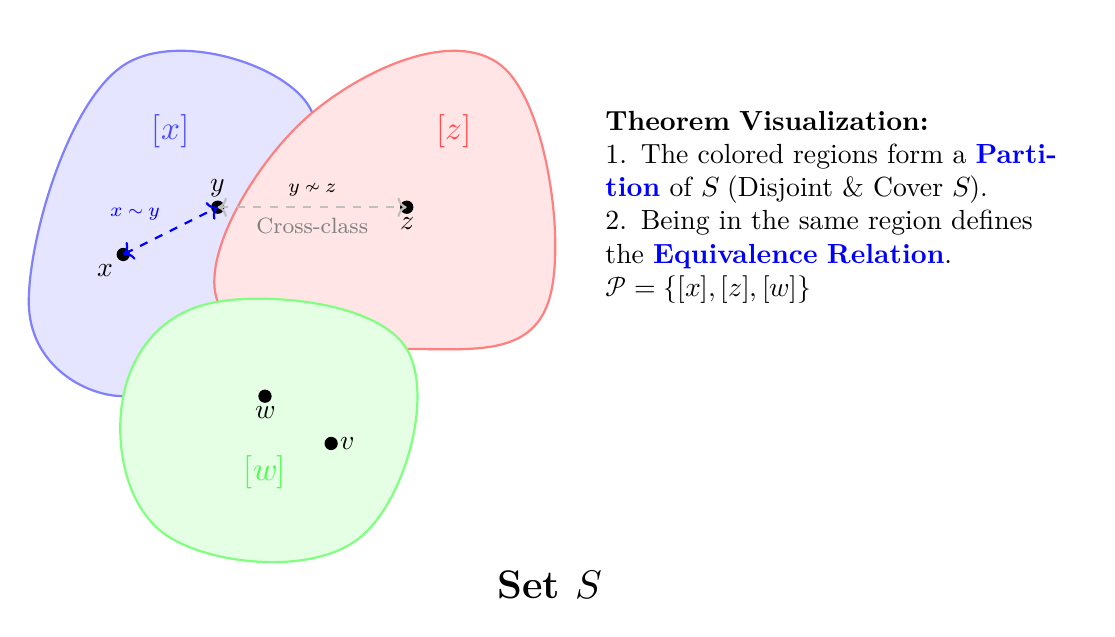
\begin{tikzpicture}[scale=1.2, every node/.style={scale=1}]
        
        % 1. Draw the main Set S (A large irregular blob)
        % We construct it by drawing individual regions that fit together
        
        % Region 1: Equivalence Class [x]
        \draw[fill=blue!10, draw=blue!50, thick, smooth cycle, tension=0.7] 
            plot coordinates {(-2,0) (-1,2.5) (1,2) (0,0) (-1,-1)};
        \node[blue!70] at (-0.5, 1.8) {\large $[x]$};
        
        % Region 2: Another Class
        \draw[fill=red!10, draw=red!50, thick, smooth cycle, tension=0.7] 
            plot coordinates {(1,2) (3,2.5) (3.5,0) (2,-0.5) (0,0)};
        \node[red!70] at (2.5, 1.8) {\large $[z]$};
        
        % Region 3: Another Class
        \draw[fill=green!10, draw=green!50, thick, smooth cycle, tension=0.7] 
            plot coordinates {(-1,-1) (0,0) (2,-0.5) (1.5,-2.5) (-0.5,-2.5)};
        \node[green!70] at (0.5, -1.8) {\large $[w]$};

        % 2. Draw Elements (Points)
        
        % Points in Region 1
        \fill (-1, 0.5) circle (2pt) node[below left] {$x$};
        \fill (0, 1) circle (2pt) node[above] {$y$};
        
        % Points in Region 2
        \fill (2, 1) circle (2pt) node[below] {$z$};
        
        % Points in Region 3
        \fill (0.5, -1) circle (2pt) node[below] {$w$};
        \fill (1.2, -1.5) circle (2pt) node[right] {$v$};

        % 3. Illustrate the Equivalence Relation
        
        % Connection between x and y (Inside the same partition)
        \draw[<->, dashed, thick, blue] (-1, 0.5) -- (0, 1) node[midway, above left, font=\scriptsize] {$x \sim y$};
        
        % No connection between x and z (Different partitions)
        \draw[<->, dashed, thick, gray!50] (0, 1) -- (2, 1) node[midway, above, font=\scriptsize, black] {$y \nsim z$};
        \node[font=\footnotesize, text=gray] at (1, 0.8) {Cross-class};

        % 4. Labels and Explanations
        \node[font=\bfseries\Large] at (3.5, -3) {Set $S$};
        
        % Arrow indicating the concept
        \node[align=left, text width=6cm, anchor=west] at (4, 1) {
            \textbf{Theorem Visualization:}\\
            1. The colored regions form a \textcolor{blue}{\textbf{Partition}} of $S$ (Disjoint \& Cover $S$).\\
            2. Being in the same region defines the \textcolor{blue}{\textbf{Equivalence Relation}}.\\
            $\mathcal{P} = \{ [x], [z], [w] \}$
        };
        
    \end{tikzpicture}
    \caption{Visualizing the equivalence between Partitions and Equivalence Relations.}
\end{figure}

\begin{definition}[Quotient Set]
Given a set $S$ and an equivalence relation $\sim$, the set of all equivalence classes is called the \textbf{Quotient Set} (商集) of $S$ by $\sim$, denoted as:
$$ S / {\sim} = \left\{ [x] \in 2^S \mid x \in S \right\} $$
\end{definition}

\begin{example}[Examples of Quotient Sets]
Here are three standard examples illustrating equivalence relations in geometry, number theory, and analysis:

\begin{enumerate}
    \item \textbf{Triangle Congruence} (三角形全等): \\
    Let $S$ be the set of all triangles in a plane. Define the relation:
    $$ T_1 \sim T_2 \iff T_1 \cong T_2 \quad (\text{$T_1$ is congruent to $T_2$}) $$
    This is an equivalence relation. The class $[T]$ represents all triangles having the same shape and size as $T$.
    
    \item \textbf{Integers Modulo 3} (模3同余): \\
    Let $S = \mathbb{Z}$. Define the relation:
    $$ m \sim n \iff m - n \text{ is divisible by } 3 $$
    The quotient set consists of exactly three elements (the residue classes):
    $$ \mathbb{Z} / {\sim} = \{ [0], [1], [2] \} $$
    
\end{enumerate}
\end{example}

\newpage

\section{Functions}

\begin{definition}[Function]
Let $A$ and $B$ be sets. A \textbf{function} (函数) (or \textit{map/mapping}) 
$$f: A \to B$$ 
is a relation $G \subseteq A \times B$ satisfying two conditions:
\begin{enumerate}
    \item \textbf{Existence:} $\forall a \in A, \exists b \in B$ such that $(a, b) \in G$.
    \item \textbf{Uniqueness (Well-defined):} If $(a, b) \in G$ and $(a, b') \in G$, then $b = b'$.
\end{enumerate}
We typically write $b = f(a)$, or $a \longmapsto b $.
The set $$G_f = \{(a, f(a)) \mid a \in A\}$$ 
is called the \textbf{graph} of $f$. We name the follows terminologies:
\begin{enumerate}
    \item \textbf{Domain} (定义域): The set $A$, denoted by $\operatorname{dom} f$.
    \item \textbf{Codomain} (陪域): The set $B$, denoted by $\operatorname{codom} f$.
    \item \textbf{Range / Image} (值域/像): The set of all value take the domain of $f$:
    $$ \operatorname{im} f = f(A) = \{ f(x) \in B \mid x \in A \} $$
\end{enumerate}
\end{definition}

\begin{definition}[Real-valued and Real Function]
    

    Let $f:A \to B$ be a function. $n$ is a positive integer.
    \begin{enumerate}
        \item If $B \subseteq \mathbb{R}$, $f$ is called a \textbf{real-valued function} (实值函数).
        \item If $B \subseteq \mathbb{R}^n$, $f$ is called a \textbf{real function} (实函数).
    \end{enumerate}

\end{definition}

\begin{remark}
    Recall that $\mathbb{R}^n = \displaystyle\prod_{r=1}^{n}\mathbb{R}$.
\end{remark}

\newcommand{\domain}{\mathrm{dom}\ }

\begin{definition}[Equal of functions]
    Let $G_f, G_g=h$ be two graphs of function $f, h$. We say $f, h$ are equal iff:
        $$G_f = G_h$$
    or equivalently, $f, h$ satisfies the follows:
    \begin{enumerate}
        \item $\domain f = \domain h$
        \item $\forall x \in \domain f ,\ f(x) = h(x) $
    \end{enumerate}
    
\end{definition}

\begin{remark}
    一般来说，函数 Codomain 的选取不影响函数的相等。即只要在定义域相同的前提下，位于 Codomain 中
    且不位于定义域中的元素不对函数的取值有任何影响。
\end{remark}

\newpage

Now we given the proof of the equlvalence of definition 3.2:
\begin{proof} Recall that $G_f = \left\{(a, f(a)) \mid a \in \domain f\right\},\
     G_h = \left\{(a, h(a)) \mid a \in \domain h\right\}$.
    \begin{align*}
        G_f = G_h &\iff \left( (a,f(a)) = (a, h(a)) \right) \land \left( \domain f = \domain h \right)\\
                  &\iff \left( f(a) = h(a) \right) \land \left( \domain f = \domain h \right)
    \end{align*}
    we have $G_f = G_h \iff \domain f = \domain h$ and $f(a) = h(a)$ , since $a \in \domain f$, so
    we done the proof.
\end{proof}


\subsection{Properties of Functions}

\begin{definition}[Classifications of Functions]
Let $f: A \to B$ be a function.
\begin{enumerate}
    \item \textbf{Injective} (单射, or one-to-one): 
    $f$ is said to \textbf{Injective} iff
    \[ \forall x, y \in A, \quad f(x) = f(y) \implies x = y \]
    
    \item \textbf{Surjective} (满射, or onto): 
        $f$ is said to \textbf{Surjective} iff
    \[ \forall y \in B, \exists\ x \in A \text{ such that } f(x) = y \quad (\text{equivalently, } f(A) = B) \]
    
    \item \textbf{Bijective} (双射, or one-to-one correspondence): $f$ is both injective and surjective.
\end{enumerate}
\end{definition}

\begin{example}

        Any line  function $f: \mathbb{R} \to \mathbb{R}$ defined by
        $$x \longmapsto mx+c$$
        is bijective, where $m \neq 0$ and $c$ are constants.
        \begin{proof}
            First we proof injective: Let $f(x) = f(y)$, then 
            $$mx+c = my +c $$
            Solve the equation, we have $x=y$. So $f$ is injective.

            Next we prove surjective: Let $y \in \mathbb{R}$, 
            we aim to show that exsits $x \in \domain f$ such that $\forall y \in \mathbb{R},f(x) = y$,
            Consider
            $$
            f(x) = y \iff mx+c = y
            $$
            Solve the equation, we have $x=\dfrac{y-c}{m}$. Then we are done.
        \end{proof}

\end{example}

\begin{example}
    We have the function $f:\mathbb{R} \to [ 0,+\infty )$ defined by
    $$ x \longmapsto x^2 $$
    is surjective not injective. The proof of surjective is so easy by solving the quadratic equation.
    For the proof of injective : Let $f(x) = f(y)$, then 
    $$x^2 = y^2$$
    Solve the equation respect by $x$, we have $x = y$ or $x = -y$. Not implies $x = y$. 
\end{example}

\newpage

The follows operation we knowed in the calculus course (MATH 1013, 1014)

\begin{definition}[Operations]\quad
\begin{enumerate}
    \item \textbf{Identity Function} (恒等函数): 
    $I_S: S \to S$ defined by $I_S(x) = x$ for all $x \in S$.
    
    \item \textbf{Composition} (复合): 
    Given $f: A \to B$ and $g: B' \to C$ with $f(A) \subseteq B'$, 
    the composition $g \circ f: A \to C$ is defined by:
    $$ (g \circ f)(x) = g(f(x)), \quad \forall x \in A $$
    
    \item \textbf{Restriction} (限制): 
    Given $f: A \to B$ and a subset $C \subseteq A$, the restriction $f|_C: C \to B$ is defined by $f|_C(x) = f(x)$ for all $x \in C$.
    
    \item \textbf{Inverse Function} (反函数): 
    If $f: A \to B$ is injective, the inverse $f^{-1}: f(A) \to A$ is defined by:
    $$ f^{-1}(y) = x \iff f(x) = y $$

    \begin{remark}
        For $f^{-1}$ to be defined on the entire codomain $B$, $f$ must be bijective.
    \end{remark}

    
\end{enumerate}

\end{definition}

Note that we have :

\begin{proposition}
    Let $f : A \to B$ be a function and $S,T \subseteq A$. Then
    \begin{enumerate}
        \item $S \subseteq T \implies f(S) \subseteq f(T)$.
        \item $f(S \cup T) = f(S) \cup f(T)$.
        \item $f(S \cap T) \subseteq f(S)\cap f(T)$.
    \end{enumerate}
\end{proposition}

\begin{proof}[Sketch of proof]\quad
    \begin{enumerate}
        \item Take $x \in S$ then $x \in T$ and $f(x) \in f(S),\ f(x) \in f(T)$.
        \item Take $x \in S \cup T$, then we can show that
        \begin{center}
            $f(S \cup T) \subseteq f(S) \cup f(T)$ and $f(S \cup T) \supseteq f(S) \cup f(T)$
        \end{center}
        \item Take $x \in S \cup T$, same to (2).
    \end{enumerate}
    \end{proof}

\begin{theorem}
        Let $f : A \to B$ and $g : B \to C$, then
        \begin{enumerate}
            \item If $g \circ f$ is surjective, then $g$ is surjective.
            \item If $g \circ f$ is injective, then $f$ is injective.
        \end{enumerate}
    \end{theorem}

    \begin{proof}\quad
        \begin{enumerate}
            \item If $g \circ f : A \to C$ surjective, then we have $g(f(A)) = C$, by $f(A) \subseteq B$ 
        we have $g(B) = C$.
            \item If $g \circ f : A \to C$ injective, then we have 
            $$\forall x,y \in A,\ g(f(x)) = g(f(y)) \implies x =y$$
            then $f(x) = f(y) \implies g(f(x)) = g(f(y)) \implies x = y$.
        \end{enumerate}
        
    \end{proof}

    \newpage

    \section{Countability}

    
    \begin{definition}[Cardinality]
    Let $A$ and $B$ be sets. The \textbf{cardinality} (基数/势), denoted by $|A|$, 
    represents the "size" of the set. 
    The relationships between cardinalities are defined via functions:

    \begin{enumerate}
        \item \textbf{Equal Cardinality} ($|A| = |B|$): \\
        Two sets have the same cardinality if and only if there exists a bijection between them.
        \[ |A| = |B| \iff \exists f: A \to B \text{ s.t. } f \text{ is bijective.} \]
        
        \item \textbf{Comparison} ($|A| \le |B|$): \\
        The cardinality of $A$ is less than or equal to $B$ if there exists an injection.
        \[ |A| \le |B| \iff \exists f: A \to B \text{ s.t. } f \text{ is injective.} \]
        
        \item \textbf{Strict Inequality} ($|A| < |B|$): \\
        \[ |A| < |B| \iff (|A| \le |B|) \land (|A| \neq |B|) \]
        This implies there exists an injection from $A$ to $B$, but no bijection exists.
    \end{enumerate}
    \end{definition}

    \begin{remark}
        集合的基数本质上是集合内元素数量拓展至无限集时的情况。
        对于有限集，基数等同于集合内的元素数量；而对于无限集，我们用“是否能建立双射”
        这一条件来分类集合的 “大小”。
    \end{remark}

    \begin{remark}
    We assign symbols to the cardinalities of common sets:
    \begin{enumerate}
        \item \textbf{Finite Sets:} If $S$ has $n$ elements, then $|S| = n$. For the empty set, $|\emptyset| = 0$.
        \item \textbf{Countable Infinity:} $|\mathbb{N}| = \aleph_0$ (Aleph-null).
        \item \textbf{The Continuum:} $|\mathbb{R}| = \mathfrak{c}$.
    \end{enumerate}
    \end{remark}

    \begin{theorem}[Schröder-Bernstein Theorem]
    If the cardinality of $A$ is less than or equal to $B$, and vice versa, then their cardinalities are equal.
    \[ (|A| \le |B|) \land (|B| \le |A|) \implies |A| = |B| \]
    \end{theorem}

    \begin{example}[Infinite Subsets]

    Consider the set of even natural numbers defined by $S = \{ 2n \mid n \in \mathbb{N} \} \subset \mathbb{N}$. 
    We have 
    \[ f: \mathbb{N} \to S \quad \text{defined by} \quad f(n) = 2n \]
    is a bijection. Therefore, $|S| = |\mathbb{N}| = \aleph_0$. The follows diagram show the meaning:
    $$
    \begin{array}{c c l}
        1 & \longrightarrow & 2\\
        2 & \longrightarrow & 4\\
        3 & \longrightarrow & 6\\
        \vdots&\vdots&\vdots 
    \end{array}
    $$
    Every element in $S$ can be respond and only respond to a number in $\mathbb{N}$
    \end{example}

    \newpage

    
    \begin{definition}[Countability]
    Let $S$ be a set.
    \begin{enumerate}
        \item \textbf{Countably Infinite(可数无穷):} $|S| = \aleph_0$. 
        There exists a bijection $f: \mathbb{N} \to S$.
        \item \textbf{Countable(可数):} $S$ is either finite or countably infinite.
        \item \textbf{Uncountable(不可数):} $S$ is not countable.
    \end{enumerate}
    \end{definition}

    \begin{remark}
        当一个集合可数时，直观意义上我们可以把所有集合的元素都“一一排列”出来。
        例如 $S={2n \mid n \in \mathbb{N}}$ 中我们可以一一列出所有的元素：
        $$ 2,4,6,8,10,12,14,\cdots $$
    \end{remark}

    \begin{example}
    The following sets are countable ($|S| = \aleph_0$):
    \begin{enumerate}
        \item \textbf{Natural Numbers} ($\mathbb{N}$): By definition.
        
        \item \textbf{Integers} ($\mathbb{Z}$): We can arrange them in a list:
        \[ 0, 1, -1, 2, -2, 3, -3, \dots \]
        Functionally, $f(n) = (-1)^n \lfloor n/2 \rfloor$ is a bijection from $\mathbb{N}$ to $\mathbb{Z}$.
        
        \item \textbf{Cartesian Product} ($\mathbb{N} \times \mathbb{N}$): 
        Using the \textbf{Diagonal Counting Scheme}, we can list pairs by traversing diagonals where $x+y$ is constant:
        \[ (1,1) \to (1,2) \to (2,1) \to (1,3) \to (2,2) \to (3,1) \to \dots \]
    \end{enumerate}
    \end{example}

    \begin{theorem}[Uncountability of the Interval]
    The open interval $(0, 1) \subset \mathbb{R}$ is uncountable.
    \end{theorem}

    \begin{proof}[\textbf{Proof (Cantor's Diagonal Argument)}]
    We proof by contradiction. Assume $(0, 1)$ is countable. 
    Then we can list all numbers in $(0,1)$ as a sequence $f(1), f(2), \dots$. Writing them in decimal expansion:
    \begin{align*}
        f(1) &= 0.\mathbf{a_{11}} a_{12} a_{13} \dots \\
        f(2) &= 0.a_{21} \mathbf{a_{22}} a_{23} \dots \\
        f(3) &= 0.a_{31} a_{32} \mathbf{a_{33}} \dots \\
        &\vdots
    \end{align*}
    Construct a new number $s = 0.b_1 b_2 b_3 \dots \in (0,1)$ such that the $n$-th digit $b_n$ differs from the diagonal digit $a_{nn}$:
    \[
    b_n = \begin{cases} 
    2 & \text{if } a_{nn} = 1 \\
    1 & \text{if } a_{nn} \neq 1 
    \end{cases}
    \]
    Since $b_n \neq a_{nn}$, $s$ differs from $f(n)$ in the $n$-th decimal place. Thus, $s \neq f(n)$ for any $n \in \mathbb{N}$. This contradicts the assumption that the list contains all numbers. Therefore, $(0,1)$ is uncountable.
    \end{proof}

    \begin{remark}
        这个证明方法最初来源于康托(Cantor's)。
        其核心是透过假设可数，然后列出所有元素，透过构造对角线元素来否定假设。
    \end{remark}

    \newpage

    \begin{theorem}[Countable Subset Theorem]
    Let $A \subseteq B$.
    \begin{enumerate}
        \item If $B$ is countable, then $A$ is countable.
        \item \textbf{Contrapositive:} If $A$ is uncountable, then $B$ is uncountable.
    \end{enumerate}
    \end{theorem}

    \begin{theorem}[Countable Union Theorem]
    The union of a countable number of countable sets is countable.
    Let $\{ A_n \}_{n \in \mathbb{N}}$ be a family of sets where each $A_n$ is countable. Then:
    \[ \bigcup_{n \in \mathbb{N}} A_n \quad \text{is countable.} \]
    \end{theorem}
    \begin{proof}[Idea of proof]
    Arrange elements in a grid (array) and use the \textbf{diagonal counting scheme} to list them.
    \end{proof}

    \begin{theorem}[Product Theorem]
    The Cartesian product of a finite number of countable sets is countable.
    \[ A, B \text{ are countable} \implies A \times B \text{ is countable.} \]
    By induction, $A_1 \times \dots \times A_n$ is countable.
    \end{theorem}

    \begin{remark}
        以上三个定理分别陈述了以下三个事实：
        \begin{enumerate}
            \item 可数集的子集依旧可数。
            \item 可数集的可数并可数。
            \item 可数集的有限积可数。
        \end{enumerate}
    \end{remark}

    \begin{example}[The Set of Rational Numbers $\mathbb{Q}$]
    The set $\mathbb{Q}$ is \textbf{countable}.
    \begin{proof}[Idea of proof]
    We can express $\mathbb{Q}$ as a countable union of countable sets:
    \[ \mathbb{Q} = \bigcup_{n \in \mathbb{N}} S_n, \quad \text{where } S_n = \left\{ \frac{m}{n} \mid m \in \mathbb{Z} \right\} \]
    Since mapping $m \mapsto \frac{m}{n}$ is a bijection from $\mathbb{Z}$ to $S_n$, each $S_n$ is countable. By Theorem 6.2, their union $\mathbb{Q}$ is countable.
    \end{proof}
    \end{example}

    \begin{example}[The Set of Irrational Numbers]
    The set $\mathbb{R} \setminus \mathbb{Q}$ is \textbf{uncountable}.
    \begin{proof}[Idea of proof]
    Assume $\mathbb{R} \setminus \mathbb{Q}$ is countable. Since $\mathbb{Q}$ is countable, their union:
    \[ \mathbb{Q} \cup (\mathbb{R} \setminus \mathbb{Q}) = \mathbb{R} \]
    would be countable (by Theorem 6.2). This contradicts the fact that $\mathbb{R}$ is uncountable.
    \end{proof}
    \end{example}

    % \begin{example}[Geometric and Algebraic Sets]
    % \begin{enumerate}
    %     \item \textbf{Complex Numbers ($\mathbb{C}$):} Uncountable. \\
    %     Since $\mathbb{R} \subset \mathbb{C}$ and $\mathbb{R}$ is uncountable, $\mathbb{C}$ must be uncountable (by Theorem 6.1).
        
    %     \item \textbf{Rational Lines:} Countable. \\
    %     The set $L = \{ y = mx + b \mid m, b \in \mathbb{Q} \}$ corresponds to pairs $(m, b) \in \mathbb{Q} \times \mathbb{Q}$. Since product of countable sets is countable, $L$ is countable.
    % \end{enumerate}
    % \end{example}

    \newpage

    \begin{example}[Power Sets and Binary Sequences]\quad
    \begin{enumerate}
        \item \textbf{Infinite Binary Sequences:} The set $B = \{ (x_1, x_2, \dots) \mid x_i \in \{0, 1\} \}$ is \textbf{uncountable} (Proven via Cantor's Diagonal Argument).
        
        \item \textbf{Power Set of $\mathbb{N}$:} The set $2^{\mathbb{N}}$ is \textbf{uncountable}. \\
        We can define a bijection $g: 2^{\mathbb{N}} \to B$ using characteristic functions. For any subset $S \subseteq \mathbb{N}$, map it to a sequence $(a_1, a_2, \dots)$ where:
        \[
        a_n = \begin{cases} 
        1 & \text{if } n \in S \\
        0 & \text{if } n \notin S 
        \end{cases}
        \]
        Note that the map is bijective. Since $B$ is uncountable, $2^{\mathbb{N}}$ is uncountable.
    \end{enumerate}
    \end{example}
    

    \begin{theorem}[Injection Theorem]
    Let $f: A \to B$ be an injective function. Then
    \[ B \text{ is countable} \implies A \text{ is countable.} \]
    \end{theorem}

    \begin{proof}[Proof Idea]
    Use the fact that $f(A) \subseteq B$ and $f: A \to f(A)$ is bijective.
    \end{proof}

    \begin{theorem}[Surjection Theorem] 
    Let $g: A \to B$ be a surjective function. Then
    \[ A \text{ is countable} \implies B \text{ is countable.} \]
    \end{theorem}

    \begin{proof}[Proof Sketch]
    Since $g$ is surjective, so $g(A) = B$. Note that 
    \[ B = \bigcup_{x \in A} \{ g(x) \} \]
    If $A$ is countable, then $B$ is a countable union of finite sets. By the \textbf{Countable Union Theorem}, $B$ is countable.
    \end{proof}

    \newpage

    \chapter{Real numbers}

    
    \section{Axioms for the Real Numbers}

    \begin{definition}[Field / 域]
    A set $F$ is a \textbf{field} if it is equipped with two 
    operations:
    $$\text{(addition)}\ + : F\times F \to F$$
    $$\text{(multiplication)}\ \cdot : F \times F \to F $$
    such that for any $a, b, c \in F$, the following axioms hold:

    \begin{enumerate}
        \item \textbf{Closure (封闭性):} \\
        $a + b \in F$ and $a \cdot b \in F$.
        
        \item \textbf{Commutativity (交换律):} \\
        $a + b = b + a$ and $a \cdot b = b \cdot a$.
        
        \item \textbf{Associativity (结合律):} \\
        $(a + b) + c = a + (b + c)$ and $(a \cdot b) \cdot c = a \cdot (b \cdot c)$.
        
        \item \textbf{Identities (单位元/幺元):} \\
        There exist unique elements $0, 1 \in F$ with $1 \neq 0$ such that:
        \[ a + 0 = a \quad \text{and} \quad a \cdot 1 = a \]
        
        \item \textbf{Additive Inverse (加法逆元):} \\
        There exists a unique element $-a \in F$ such that $a + (-a) = 0$.
        
        \item \textbf{Multiplicative Inverse (乘法逆元):} \\
        For any $a \neq 0$, there exists a unique element $a^{-1} \in F$ such that $a \cdot (a^{-1}) = 1$.
        
        \item \textbf{Distributivity (分配律):} \\
        $a \cdot (b + c) = a \cdot b + a \cdot c$.
    \end{enumerate}
    \end{definition}

    \begin{remark}
        $\mathbb{R}, \mathbb{Q}$ 构成一个域，即它满足上述定义所说的所有公理。
    \end{remark}

    \newpage

    We can define a "natural order" on $\mathbb{Q}$ (and $\mathbb{R}$) compatible with arithmetic operations. This structure is called an \textbf{Ordered Field} (有序域).

    \begin{definition}[Ordered Field / 有序域]
    A field $F$ is an \textbf{ordered field} if there exists an order relation $<$ such that for any $a, b, c \in F$:

    \begin{enumerate}
        \item \textbf{Trichotomy (三歧性):} \\
        Exactly one of the following holds:
        \[ a < b, \quad a = b, \quad \text{or} \quad b < a \]
        
        \item \textbf{Transitivity (传递性):} \\
        If $a < b$ and $b < c$, then $a < c$.
        
        \item \textbf{Compatibility with Addition (加法相容性):} \\
        If $a < b$, then $a + c < b + c$.
        
        \item \textbf{Compatibility with Multiplication (乘法相容性):} \\
        If $a < b$ and $0 < c$, then $ac < bc$.
    \end{enumerate}
    \end{definition}

    \begin{remark}
        同样，$\mathbb{R}, \mathbb{Q}$ 构成一个有序域。
    \end{remark}

    \begin{definition}[Basic Notations / 基本记号]
    Suppose $F$ is an ordered field. For any $a, b, a_i \in F$ ($i=1, \dots, n$), we define:

    \begin{enumerate}
        \item \textbf{Strict Inequality (严格不等式):} \\
        $$a > b \iff b < a$$
        
        \item \textbf{Less than or Equal (小于等于):} \\
        $$a \le b \iff a < b \text{ or } a = b$$
        
        \item \textbf{Greater than or Equal (大于等于):} \\
        $$a \ge b \iff a > b \text{ or } a = b$$
        
        \item \textbf{Closed Interval (闭区间):} \\
        $$[a, b] = \{ x \in F \mid a \le x \le b \}$$
        
        \item \textbf{Open Interval (开区间):} \\
        $$(a, b) = \{ x \in F \mid a < x < b \}$$
        
        \item \textbf{Maximum (最大值):} 
        $\max(a_1, \dots, a_n)$ is the largest element among $a_1, \dots, a_n$.
        
        \item \textbf{Minimum (最小值):} 
        $\min(a_1, \dots, a_n)$ is the smallest element among $a_1, \dots, a_n$.
        
        \item \textbf{Absolute Value (绝对值):} \\
        $$|a| = \max(a, -a) = \begin{cases} a & \text{if } a \ge 0 \\ -a & \text{if } a < 0 \end{cases}$$
    \end{enumerate}
    \end{definition}

    \newpage

    We have some propositions about the inequality:

    \begin{proposition}[Properties of Inequalities ]
    Suppose $F$ is an ordered field. For any $a, b, c, d \in F$:

    \begin{enumerate}
        \item \textbf{Addition of Inequalities (不等式的加法):} If $a < b$ and $c < d$, then 
        \begin{center}
            $a + c < b + d$
        \end{center}
        
        
        \item \textbf{Positivity of Squares (平方非负性):} If $a \neq 0$, then
        \begin{center}
            $a^2 > 0$
        \end{center}
        

        \item \textbf{Sign Flip (变号):} 
        \begin{center}
            $a > 0 \iff -a < 0$
        \end{center}
        
        \item \textbf{Multiplication by Negative (乘以负数变号):} If $c < 0$ and $a < b$, then
        \begin{center}
             $ac > bc$
        \end{center}
        
        \item \textbf{Reciprocals Revert Order (倒数反序):} If $0 < a < b$, then 
        \begin{center}
            $0 < b^{-1} < a^{-1}$ 
        \end{center}
        
        \item \textbf{Absolute Value Bounds (绝对值界限):} 
        \begin{center}
            $-|a| \le a \le |a|$
        \end{center}
        
        \item \textbf{Bounded by Constant (常数界限):} 
        \begin{center}
            $|a| \le b \iff -b \le a \le b$
        \end{center}
        
        \item \textbf{Outside Bounds (外部界限):}
        \begin{center}
            $|a| \ge b \iff a \le -b \text{ or } a \ge b$
        \end{center}
       
        
        \item \textbf{Triangle Inequality (三角不等式):}
        \begin{center}
            $|a + b| \le |a| + |b|$
        \end{center}
        
        \item \textbf{Reverse Triangle Inequality (反向三角不等式):} 
        \begin{center}
            $|a - b| \ge \big| |a| - |b| \big|$ 
        \end{center}
    \end{enumerate}
    \end{proposition}

    Proof is obviously.

    \newpage

    \subsection{Supremum and infimum}

    \begin{definition}[Boundedness / 有界性]
    Let $F$ be an ordered field and $E \subseteq F$.

    \begin{enumerate}
        \item \textbf{Bounded Above (有上界):} \\
        If there exists $\beta \in F$ such that $x \le \beta$ for all $x \in E$, we say that $E$ is \textit{bounded above}. The element $\beta$ is called an \textbf{upper bound} (上界) of $E$.
        
        \item \textbf{Bounded Below (有下界):} \\
        If there exists $\beta \in F$ such that $x \ge \beta$ for all $x \in E$, we say that $E$ is \textit{bounded below}. The element $\beta$ is called a \textbf{lower bound} (下界) of $E$.
        
        \item \textbf{Bounded (有界):} \\
        $E$ is said to be \textit{bounded} if it is both bounded above and bounded below.
    \end{enumerate}
    \end{definition}

    \begin{example}
        Obviously, we have the follows results:
        \begin{enumerate}
            \item Any open interval $(a,b)$ is bounded on $\mathbb{R}$. 
            This result also hold on colsed and half interval.

            \item $\mathbb{Q}, \mathbb{N}, \mathbb{Z},\mathbb{R}$ not bounded on $\mathbb{R}$.
        \end{enumerate}
    \end{example}



    \begin{definition}[Supremum / 上确界]
    Let $E \subseteq F$ such that $E$ is bounded above. Suppose there exists $\alpha \in F$ such that:
    \begin{enumerate}
        \item $\alpha$ is an upper bound of $E$ (i.e., $\forall x \in E, x \le \alpha$).
        \item If $\gamma < \alpha$, then $\gamma$ is \textbf{not} an upper bound of $E$ (i.e., $\exists x \in E$ such that $x > \gamma$).
    \end{enumerate}
    Then $\alpha$ is called the \textbf{least upper bound} (最小上界) of $E$, or the \textbf{supremum} of $E$, denoted as $\alpha = \sup E$.
    \end{definition}

    \begin{definition}[Infimum / 下确界]
    Similarly, suppose $E$ is bounded below and there exists $\alpha \in F$ such that:
    \begin{enumerate}
        \item $\alpha$ is a lower bound of $E$ (i.e., $\forall x \in E, x \ge \alpha$).
        \item If $\gamma > \alpha$, then $\gamma$ is \textbf{not} a lower bound of $E$.
    \end{enumerate}
    Then $\alpha$ is called the \textbf{greatest lower bound} (最大下界) of $E$, or the \textbf{infimum} of $E$, denoted as $\alpha = \inf E$.
    \end{definition}

    \begin{remark}
        上下确界的概念相当于集合的“边界”，直观上，上下确界“夹紧”了一个集合。
        注意并非每一个有序域中的子集都具有上下确界。
    \end{remark}

    \begin{center}
    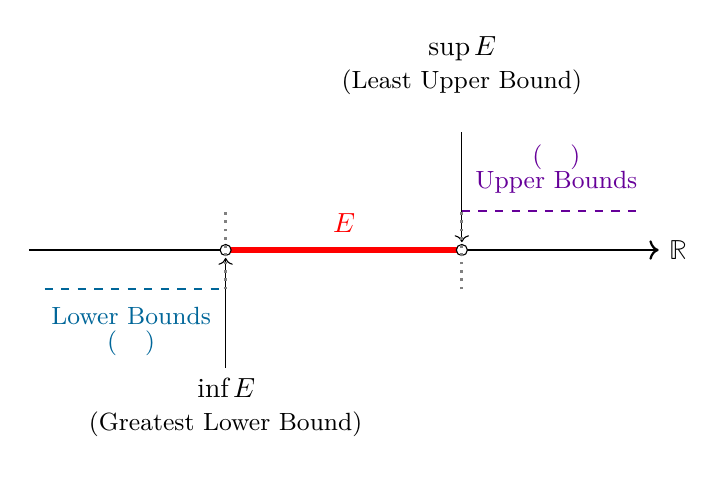
\begin{tikzpicture}[scale=1]
        % Draw the Real Line (数轴)
        \draw[->, thick] (-4,0) -- (4,0) node[right] {$\mathbb{R}$};
        
        % Draw Set E (集合 E) - 假设是一个开区间 (a, b)
        \draw[red, line width=2.5pt] (-1.5,0) -- (1.5,0);
        \node[red, above] at (0,0.1) {$E$};
        
        % Draw Lower Bounds (下界区域)
        \draw[dashed, blue!60!green, thick] (-3.8,-0.5) -- (-1.5,-0.5);
        \node[blue!60!green, below] at (-2.7,-0.6) {\small Lower Bounds};
        \node[blue!60!green, below] at (-2.7,-0.9) {\small (下界集合)};
        
        % Draw Upper Bounds (上界区域)
        \draw[dashed, blue!60!red, thick] (1.5,0.5) -- (3.8,0.5);
        \node[blue!60!red, above] at (2.7,0.6) {\small Upper Bounds};
        \node[blue!60!red, above] at (2.7,0.9) {\small (上界集合)};

        % Indicate Infimum
        \draw[fill=white] (-1.5,0) circle (2pt); % Open circle for boundary
        \draw[<-] (-1.5,-0.1) -- (-1.5,-1.5) node[below, align=center] {
            $\inf E$ \\ \small (Greatest Lower Bound) \\ \small 最大的下界
        };

        % Indicate Supremum
        \draw[fill=white] (1.5,0) circle (2pt); % Open circle for boundary
        \draw[<-] (1.5,0.1) -- (1.5,1.5) node[above, align=center] {
            $\sup E$ \\ \small (Least Upper Bound) \\ \small 最小的上界
        };

        % Highlighting "The Boundary"
        \draw[line width=1pt, gray, dotted] (-1.5, -0.5) -- (-1.5, 0.5);
        \draw[line width=1pt, gray, dotted] (1.5, -0.5) -- (1.5, 0.5);

    \end{tikzpicture}
    \end{center}
    \newpage
    
    Now we given some example:

    \begin{example}\quad
            \item The open interval $A=(0,1)$ has supremum $1$ and infimum $0$. i.e.
            $$
            \inf A = 0,\ \sup A = 1
            $$
            \begin{proof}
                We just prove the part of supremum: Suppose $s = \sup A \neq 1$, 
                then we want to prove $s<1$ and $s>1$ both not least upper bound.
                \begin{enumerate}
                    \item If $s<1$: Note that there are $x \in A$ s.t $s<x<1$ since
                    $$ s < \dfrac{s+1}{2} < 1$$
                    so $s<1$ not upper bounded of $A$.
                    \item If $s>1$: Note that there are $x > 1$ s.t $1<x<s$ since
                    $$ 1 < \dfrac{s+1}{2} < s$$
                    so $s>1$ is upper bounded of $A$, but not least upper bound of $A$.
                \end{enumerate}
            \end{proof}
            \begin{remark}
                一般而言，证明某个集合的下确界通常需要用到反证法，
                对每种不同的情况构造一些数说明其并非上界或最小上界。
            \end{remark}
    \end{example}

    \subsection{The Completeness Axiom}

    \begin{definition}[Completeness Axiom / 完备性公理]
    An ordered field $F$ is said to be \textbf{complete} (完备的) 
    if every nonempty subset of $F$ which is bounded above has a supremum in $F$.

    \end{definition}

    \begin{remark}
        即完备域要求对域中任意的子集，其上下确界都在域中存在。
    \end{remark}

    \begin{example}
        Consider $\mathbb{Q}$, there are not complete. Sinec
        $$
        S = \{ x \mid x^2 < 2 \}
        $$
        not supremum, since $\sqrt{2} \notin \mathbb{Q}$.
    \end{example}

    \newpage

    \section{Properties of Real Numbers}

    The following properties are direct consequences of the field axioms and the order axiom.

    \subsection{The Infinitesimal Principle}

    \begin{theorem}[Infinitesimal Principle / 无穷小原理]
    For $x, y \in \mathbb{R}$,
    \[ x < y + \epsilon \quad \text{for all } \epsilon > 0 \iff x \le y. \]
    \end{theorem}

    \begin{proof}
    \textbf{($\Leftarrow$):} Obviously.
    % If $x \le y$, then naturally for any $\epsilon > 0$, we have $x \le y < y + \epsilon$. 
    % Thus the inequality holds.
    \end{proof}
    \begin{proof}
        \textbf{($\Rightarrow$):}
        We prove by contradiction. 
        Assume that $x > y$. Let $\epsilon_0 = x - y$. Since $x > y$, we have $\epsilon_0 > 0$. 
        Put $\epsilon_0$ into the hypothesis:
        \[ x < y + \epsilon_0 = y + (x - y) = x \]
        This implies $x < x$, which is a contradiction. Therefore, we must have $x \le y$.
    \end{proof}

    \begin{remark}
        证明的关键是透过选取合适的 $\epsilon>0$ 构造矛盾。利用了 $\epsilon$ 的任意性。
    \end{remark}

    \begin{remark}
    Using the infinitesimal principle, it is easy to see that:
    \[ |x| < \epsilon \quad \text{for all } \epsilon > 0 \iff x = 0. \]
    \end{remark}

    \subsection{Approximation Properties of Supremum and Infimum }

    These theorems provide a practical way to check if a number is the supremum or infimum using an arbitrarily small number $\epsilon$.

    \begin{theorem}[Supremum Property / 上确界性质]
    Suppose $S \subseteq \mathbb{R}$ and $U$ is an upper bound of $S$.
    \[ U = \sup S \iff \forall \epsilon > 0, \exists x \in S \text{ such that } U - \epsilon < x. \]
    \end{theorem}

    \begin{proof}
    \textbf{($\Rightarrow$):} We have
    $$ \forall \epsilon > 0,\ U - \epsilon<U $$
    Therefore, $U - \epsilon$ not upper bound of $S$. 
    So there exsits $x \in S$ s.t $ x >U - \epsilon$.
    \end{proof}
    \begin{proof}
    \textbf{($\Leftarrow$):} 
    Let $U' = \sup S$. Since $U$ is an upper bound, so $U \ge U'$. \\
    For any $\epsilon > 0$, by our hypothesis, there exists $x \in S$ such that $U - \epsilon < x$. \\
    Since $x \le \sup S = U'$, we have:
    \[ U - \epsilon < x \le U' \implies U < U' + \epsilon \]
    Since this holds for all $\epsilon > 0$, by the \textbf{Infinitesimal Principle}, we have $U \le U'$. \\
    Combining $U \ge U'$ and $U \le U'$, we conclude $U = U'$.
    \end{proof}

    \begin{theorem}[Infimum Property / 下确界性质]
    Suppose $S \subseteq \mathbb{R}$ and $L$ is a lower bound of $S$.
    \[ L = \inf S \iff \forall \epsilon > 0, \exists x \in S \text{ such that } L + \epsilon > x. \]
    \end{theorem}

    \begin{proof}
    The proof is symmetric to the proof of the Supremum Property.
    \end{proof}

    \newpage

    \section{Algebraic Properties of Supremum and Infimum}

    \begin{proposition}[Reflection / Negation(反射/取负) Properties]
    Let $B$ be nonempty subset of $\mathbb{R}$.
    Define $-B = \{-x \in \mathbb{R} \mid x \in B\}$.
        \begin{enumerate}
            \item If $B$ is bounded below, then $-B$ is bounded above, and
            \[ \inf B = -\sup(-B)\]
            \item If $B$ is bounded above, then $-B$ is bounded below, and
            \[ \sup B = -\inf(-B)\]
        \end{enumerate}
    
    \end{proposition}

    \begin{center}
    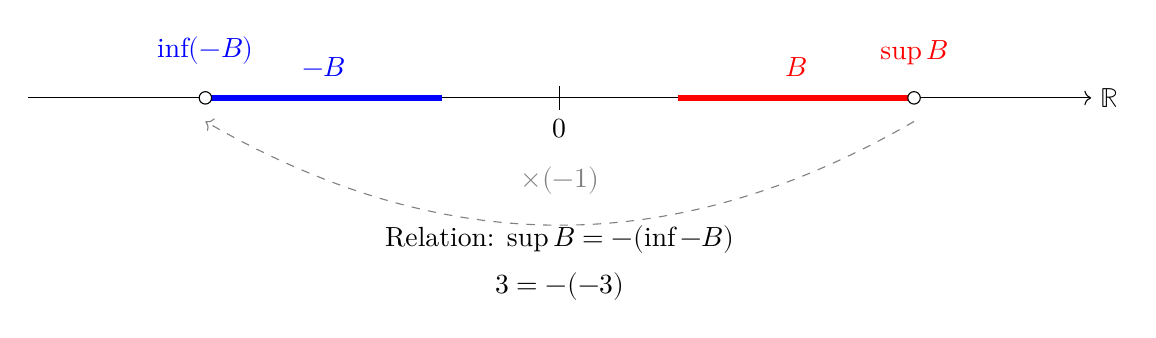
\begin{tikzpicture}[scale=1.5]
        % Axis
        \draw[->] (-4.5,0) -- (4.5,0) node[right] {$\mathbb{R}$};
        \draw (0,0.1) -- (0,-0.1) node[below] {$0$};

        % Set B (Original)
        \draw[red, line width=2pt] (1,0) -- (3,0);
        \node[red, above] at (2,0.1) {$B$};
        \draw[fill=white] (3,0) circle (1.5pt); % boundary
        \node[red, above] at (3,0.2) {$\sup B$};

        % Set -B (Reflected)
        \draw[blue, line width=2pt] (-3,0) -- (-1,0);
        \node[blue, above] at (-2,0.1) {$-B$};
        \draw[fill=white] (-3,0) circle (1.5pt); % boundary
        \node[blue, above] at (-3,0.2) {$\inf(-B)$};

        % Arrows showing reflection
        \draw[->, dashed, gray] (3,-0.2) to[bend left] (-3,-0.2);
        \node[gray, below] at (0,-0.5) {$\times (-1)$};

        % Relationship
        \node at (0, -1.2) {Relation: $\sup B = - (\inf -B)$};
        \node at (0, -1.6) {$3 = -(-3)$};
    \end{tikzpicture}
    \end{center}

    \begin{remark}
        直观理解：将集合绕原点翻转，原来的“最右端”（上确界）变成了新集合的“最左端”（下确界）的负数。
    \end{remark}

    \begin{proof}[Sketch of proof]
        If $B$  bounded below, then $\inf B$ exists. By Infimum Property:
        $$
        \forall \epsilon > 0, \exists x \in B, x < \inf B +\epsilon
        $$
        so $ -x > -\inf B -\epsilon$, obviously that $-B$ is bounded above, so $\sup(-B)$ exists.
        Since $-x \in (-B)$ we have $-\inf B = \sup(-B)$ by Supremum Property and we done the proof.
        \\

        Another case is symmetric to the proof of above.
        
    \end{proof}

    \begin{remark}
        本定理的证明体现了下确界与上确界性质的应用。此性质是确界的准确代数表示。
    \end{remark}

    \newpage

    We have more properties:
    
    \begin{proposition}[Operations on Sets and Bounds]
        Let $A$ and $B$ be nonempty subsets of $\mathbb{R}$.

    \begin{enumerate}
        \item \textbf{Scalar Multiplication (非负数乘):} 
        Let $c \ge 0$. Define $cB = \{cx \in \mathbb{R} \mid x \in B\}$.
        \begin{itemize}
            \item If $B$ is bounded above, then:
            \[ \sup(cB) = c \sup B. \]
        \end{itemize}
        \textit{(Note: Similarly for infimum: $\inf(cB) = c \inf B$ if $c \ge 0$.)}

        \begin{center}
        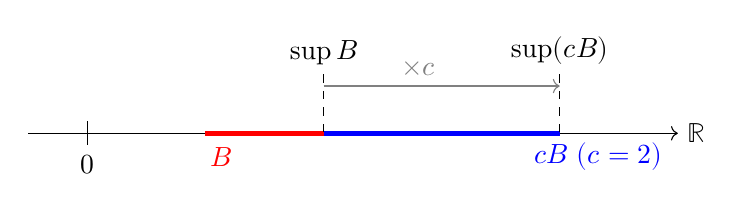
\begin{tikzpicture}[scale=1.5]
            % Axis
            \draw[->] (-0.5,0) -- (5,0) node[right] {$\mathbb{R}$};
            \draw (0,0.1) -- (0,-0.1) node[below] {$0$};

            % Set B
            \draw[red, line width=2pt] (1,0) -- (2,0);
            \node[red, left] at (1.3,-0.2) {$B$};
            \draw[dashed] (2,0.5)node[above] {$\sup B$} -- (2,0) ;

            % Set cB (Scaled by 2)
            \draw[blue, line width=2pt] (2,0) -- (4,0);
            \node[blue, right] at (3.7,-0.2) {$cB \ (c=2)$};
            \draw[dashed] (4,0.5)node[above] {$\sup(cB)$} -- (4,0) ;

            % Expansion arrows
            \draw[->, gray, thin] (2,0.4) -- (4,0.4);
            \node[gray, above] at (2.8,0.4) {$\times c$};
        \end{tikzpicture}
        \end{center}

        \item \textbf{Subsets (子集性质):} 
        Suppose $\emptyset \neq A \subseteq B$.
        \begin{itemize}[itemsep=0.5em, topsep=0.5em, partopsep=0.25em]
            \item If $B$ is bounded below, then $\inf B \le \inf A$.
            \item If $B$ is bounded above, then $\sup A \le \sup B$.
        \end{itemize}
        
        \begin{center}
        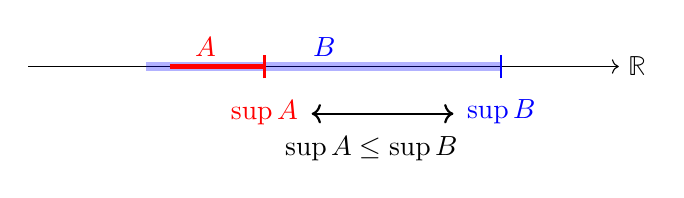
\begin{tikzpicture}[scale=1.5]
            % Axis
            \draw[->] (0,0) -- (5,0) node[right] {$\mathbb{R}$};

            % Set B (Larger)
            \draw[blue, line width=3pt, opacity=0.3] (1,0) -- (4,0);
            \node[blue, above] at (2.5,0) {$B$};
            \draw[blue, thick] (4, -0.1) -- (4, 0.1);
            \node[blue, below] at (4,-0.2) {$\sup B$};

            % Set A (Smaller, inside)
            \draw[red, line width=1.5pt] (1.2,0) -- (2,0);
            \node[red, above] at (1.5,0) {$A$};
            \draw[red, thick] (2, -0.1) -- (2, 0.1);
            \node[red, below] at (2,-0.2) {$\sup A$};

            % Inequality visual
            \draw[<->, thick, black] (2.4, -0.4) -- (3.6, -0.4);
            \node[below] at (2.9, -0.5) {$\sup A \le \sup B$};
        \end{tikzpicture}
        \end{center}


        \item \textbf{Translation (平移):} 
        Let $c \in \mathbb{R}$. Define $c + B = \{c + x \in \mathbb{R} \mid x \in B\}$.
        \begin{itemize}[itemsep=0.5em, topsep=0.5em, partopsep=0.25em]
            \item $\sup(c + B) = c + \sup B$.
            \item $\inf(c + B) = c + \inf B$.
        \end{itemize}
        

        \item \textbf{Minkowski Sum (集合加法):} 
        Define $A + B = \{x + y \in \mathbb{R} \mid x \in A, y \in B\}$.
        \begin{itemize}
            \item If $A$ and $B$ are bounded, then:
            \[ \sup(A + B) = \sup A + \sup B \]
            \[ \inf(A + B) = \inf A + \inf B \]
        \end{itemize}

        \begin{center}
        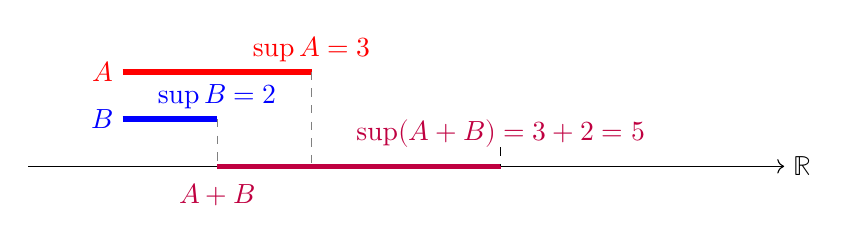
\begin{tikzpicture}[scale=1.2]
            % Axis
            \draw[->] (0,0) -- (8,0) node[right] {$\mathbb{R}$};

            % Set A
            \draw[red, line width=2pt] (1,1) -- (3,1);
            \node[red, left] at (1,1) {$A$};
            \node[red, above] at (3,1) {$\sup A=3$};

            % Set B
            \draw[blue, line width=2pt] (1,0.5) -- (2,0.5);
            \node[blue, left] at (1,0.5) {$B$};
            \node[blue, above] at (2,0.5) {$\sup B=2$};

            % Set A+B
            % Range: [1+1, 3+2] = [2, 5]
            \draw[purple, line width=2pt] (2,0) -- (5,0);
            \node[purple, left] at (2.5,-0.3) {$A+B$};
            \draw[dashed] (5,0.2) -- (5,0); 
            \node[purple, above] at (5,0.1) {$\sup(A+B) = 3+2 = 5$};

            % Visual connection
            \draw[dashed, gray] (3,1) -- (3,0);
            \draw[dashed, gray] (2,0.5) -- (2,0);
            
            % Brace to show addition (这里需要 decorations.pathreplacing 库)
            % \draw[decorate,decoration={brace,amplitude=5pt}] (1,1.4) -- (3,1.4) node[midway, above=5pt] {\small max reach of A};
            % \draw[decorate,decoration={brace,amplitude=5pt}] (3,1.4) -- (5,1.4) node[midway, above=5pt] {\small + max reach of B};
        \end{tikzpicture}
        \end{center}

    \end{enumerate}
    \end{proposition}

    \newpage
    
    \section{Well-Order Principle}

    \begin{definition}[Well-ordering Axiom / 良序公理]
    The set of natural numbers $\mathbb{N}$ is \textit{well-ordered}. This means that for any nonempty subset $S \subseteq \mathbb{N}$, there exists a \textbf{least element} (minimum) in $S$.
    \[ \forall S \subseteq \mathbb{N}, S \neq \emptyset \implies \exists m \in S \text{ s.t. } \forall x \in S, m \le x. \]
    \end{definition}

    \begin{remark}
        可以认为良序公理中的最小元素即是 $S$ 的下确界。换言之良序公理说明任何自然数集的子集都有下确界。
    \end{remark}

    \subsection{Mathematical Induction}

    \begin{theorem}[Mathematical Induction / 数学归纳法]
    Let $P(n)$ be a statement (proposition) depending on $n \in \mathbb{N}$. Suppose :
    \begin{enumerate}
        \item \textbf{Base Case:} $P(1)$ is true.
        \item \textbf{Inductive Step (归纳步骤):} For any $k \in \mathbb{N}$, if $P(k)$ is true, then $P(k+1)$ is true.
        \[ \forall k \in \mathbb{N}, P(k) \implies P(k+1) \]
    \end{enumerate}
    Then, $P(n)$ is true for all $n \in \mathbb{N}$. Or use the logic symbols:
    \[  \left[ \left( P(1) = \mathbb{T}\right) \land \left( \forall k \in \mathbb{N}, P(k)= \mathbb{T} \implies P(k+1)= \mathbb{T} \right)  \right] \implies \forall n \in \mathbb{N}, P(n) = \mathbb{T} \]
    \end{theorem}

    \begin{proof}
    We prove this by contradiction using the Well-ordering Axiom.

    Assume that $P(n)$ is not true for some $n$. Define the set of counterexamples:
    \[ S = \{ n \in \mathbb{N} \mid P(n) \text{ is false} \} \]
    By our assumption, $S \neq \emptyset$. By the \textbf{Well-ordering Axiom}, $S$ must have a least element, let's call it $m = \min S$.

    \begin{enumerate}
        \item Since $P(1)$ is true (by Condition 1), $1 \notin S$. Thus, $m > 1$ (or $m \ge 2$).
        \item Consider the number $k = m - 1$. Since $m > 1$, $k \in \mathbb{N}$.
        Because $k < m$ and $m$ is the least element of $S$,so $P(k)$ is true.
        We have $P(k+1) = P(m)$ is true.
    \end{enumerate}
    However, $m \in S$ implies $P(m)$ is false. This is a contradiction. Therefore, the set $S$ must be empty, meaning $P(n)$ is true for all $n$.
    \end{proof}

    \begin{remark}
        该证明的核心原理是透过反证法假设在 \textbf{Base Case}与 \textbf{Inductive Step} 成立的前提下
        仍然存在某些不正确的命题。将这些不正确的命题看作一个集合，使用良序公理导出矛盾。
    \end{remark}

    \begin{remark}
        事实上 \textbf{Base Case} 中初始命题并不依赖数字 $1$。换言之，只要 $\exists r\geq 1, P(r) = \mathbb{T}$ 
        以及 \textbf{Inductive Step} 成立，则 $\forall n \geq r, P(n) = \mathbb{T}$.
    \end{remark}

    \begin{remark}
        这不代表该命题在 $n=+\infty$ 时成立。数学归纳法只针对有限的情况。
    \end{remark}

    \newpage

    \subsection{Archimedean Principle}

    
    \begin{theorem}[Archimedean Principle / 阿基米德原理]
    For any real number $x \in \mathbb{R}$, there exists a natural number $n \in \mathbb{N}$ strictly greater than $x$.
    \[ \forall x \in \mathbb{R}, \exists n \in \mathbb{N} \text{ s.t. } n > x. \]
    \end{theorem}

    \begin{proof}
    We prove by contradiction.
    Assume the statement is false, i.e.
    $$\forall n \in \mathbb{N}, n \le x$$
    This implies that $x$ is an upper bound of $\mathbb{N}$. By the \textbf{Completeness Axiom}, $\sup \mathbb{N}$ exists in $\mathbb{R}$. Let $S = \sup \mathbb{N}$.

    By Supremum Property, there exists some $m \in \mathbb{N}$ such that:
    \[ m > S - 1 \]
    So we have $m + 1 > S$.
    Since $m \in \mathbb{N}$, we have $m+1 \in \mathbb{N}$. This contradicts the fact that $S$ is an upper bound for all natural numbers.
    \end{proof}

    \begin{remark}
        阿基米德原理说明 $\mathbb{N}$ 是无界的，即不存在最大的正整数。
    \end{remark}

    \begin{corollary}[Arbitrarily Small Numbers]
    For any positive real number $\epsilon > 0$, there exists a natural number $n \in \mathbb{N}$ such that:
    \[ 0 < \frac{1}{n} < \epsilon \]
    \end{corollary}

    \begin{proof}
        Apply the Archimedean Principle with $x = \frac{1}{\epsilon}$. 
        There exists $n > \frac{1}{\epsilon}$, which implies $\frac{1}{n} < \epsilon$.
    \end{proof}

    Using the Archimedean Principle and the Well-ordering Principle, we can define the integer parts of any real number.

    \begin{lemma}[Ceiling and Floor / 向上取整与向下取整]
    For any $x \in \mathbb{R}$:
    \begin{enumerate}
        \item There exists a unique integer $m$ such that $m-1 < x \le m$. This $m$ is called the \textbf{ceiling} of $x$, denoted by $\lceil x \rceil$.
        \item There exists a unique integer $k$ such that $k \le x < k+1$. This $k$ is called the \textbf{floor} of $x$, denoted by $\lfloor x \rfloor$.
    \end{enumerate}
    \end{lemma}

    \newpage
    

    \subsection{Density of Rational and Irrational Numbers}

    A subset $S \subseteq \mathbb{R}$ is said to be \textbf{dense} (稠密) in $\mathbb{R}$ if between any two distinct real numbers, there exists an element of $S$.

    \begin{theorem}[Density of Rational Numbers / 有理数的稠密性]
    If $x, y \in \mathbb{R}$ and $x < y$, then there exists a rational number $q \in \mathbb{Q}$ such that $x < q < y$.
    \end{theorem}

    \begin{analysis}
    We want to prove $x<q<y$. Note that 
    $$
    x<y \iff y-x>0
    $$
    Use Corollary 2.1 we have there exist a $n \in \mathbb{N}$ s.t $0<\dfrac{1}{n}<y-x \implies nx + 1 < ny$.
    \end{analysis}

    \begin{proof}
    By above analysis we have:
    \begin{align*}
                 &nx + 1 < ny \\
        \implies & nx <\lfloor nx \rfloor +1 <nx+1 <ny \\
        \implies & nx <\lfloor nx \rfloor +1 <ny \\
        \implies & x <\dfrac{\lfloor nx \rfloor +1}{n} <y 
    \end{align*}
    Note that $\dfrac{\lfloor nx \rfloor +1}{n} \in \mathbb{Q}$, we complete the proof.
    \end{proof}

    \begin{remark}
        
    \end{remark}

    \begin{theorem}[Density of Irrational Numbers / 无理数的稠密性]
    If $x, y \in \mathbb{R}$ and $x < y$, then there exists an irrational number $w \in \mathbb{R} \setminus \mathbb{Q}$ such that $x < w < y$.
    \end{theorem}

    \begin{proof}[Sketch of proof]
    Fixed irrational number $w_0 > 0$ and use theorem 2.6 for $\dfrac{x}{w}<\dfrac{y}{w}$.
    \end{proof}

    \begin{example}[Infimum of Reciprocals]
    Let $S = \{ \frac{1}{n} \mid n \in \mathbb{N} \}$. Show that $\inf S = 0$.
    \begin{proof}
        
        Clearly, $\dfrac{1}{n} > 0$ for all $n$, so $0$ is a lower bound.
        Let $t > 0$ be a lower bound.

        By the Archimedean Principle, there exists $n \in \mathbb{N}$ such that $n > \dfrac{1}{t}$.
        $\dfrac{1}{n} < t$

        Since $\dfrac{1}{n} \in S$, $t$ cannot be a lower bound (contradiction).
        Thus, $\inf S = 0$.
    \end{proof}
    \end{example}

    \begin{example}[Supremum of a Rational Set]
    Let $T = [2, 3) \cap \mathbb{Q}$. Show that $\sup T = 3$.

    \begin{proof}
    Clearly that $3$ is an upper bound. Let  $u < 3$ is supremum.

    We have an interval $(u, 3)$. By the \textbf{Density of Rationals}, 
    there exists $r \in \mathbb{Q}$ such that $u < r < 3$.

    Clearly, $r \in \mathbb{Q}$, contradicts that $u$ is an upper bound.Thus, $\sup T = 3$.
    \end{proof}

    \end{example}

    \newpage

    \chapter{Sequences and Series}

    \section{Limit of Sequences}

    \subsection{Definition}

    \begin{definition}[Sequence and Boundedness / 数列与有界性]
    An \textbf{infinite sequence} (数列) $\{a_n\}$ is a function $f: \mathbb{N} \to \mathbb{R}$ where $a_n = f(n)$.

    The sequence $\{a_n\}$ is:
    \begin{itemize}
        \item \textbf{Bounded above (有上界):} if the set $\{a_n \mid n \in \mathbb{N}\}$ is bounded above.
        \[ \sup \{a_n\} = \sup \{ a_n \in \mathbb{R} \mid n \in \mathbb{N} \} < \infty \]
        \item \textbf{Bounded below (有下界):} if the set $\{a_n \mid n \in \mathbb{N}\}$ is bounded below.
        \[ \inf \{a_n\} = \inf \{ a_n \in \mathbb{R} \mid n \in \mathbb{N} \} > -\infty \]
    \end{itemize}
    \end{definition}

    \begin{definition}[Distance and Neighborhood / 距离与邻域]
    For $x, y \in \mathbb{R}$, the \textbf{distance} is defined as $d(x,y) = |x - y|$. \\
    For $c \in \mathbb{R}$ and $\varepsilon > 0$, the \textbf{$\varepsilon$-neighborhood} of $c$ is the open interval $(c-\varepsilon, c+\varepsilon)$.
    \[ x \in (c-\varepsilon, c+\varepsilon) \iff |x - c| < \varepsilon \]
    \end{definition}

    \begin{definition}[Convergence / 收敛]
    A sequence $\{a_n\}$ \textbf{converges} to a real number $l$ (denoted $\lim_{n \to \infty} a_n = l$ or $a_n \to l$) if and only if:
    \[ \forall \varepsilon > 0, \exists N \in \mathbb{N} \text{ such that } \forall n \ge N, |a_n - l| < \varepsilon. \]
    \end{definition}



    \begin{definition}[Divergence / 发散]
    If a sequence does not converge to a finite limit, it \textbf{diverges}.
    \begin{itemize}
        \item \textbf{Diverges to $\infty$:} $\forall A \in \mathbb{R}, \exists N \in \mathbb{N}, \forall n \ge N, a_n > A$.
        \item \textbf{Diverges to $-\infty$:} $\forall A \in \mathbb{R}, \exists N \in \mathbb{N}, \forall n \ge N, a_n < A$.
    \end{itemize}
    \end{definition}

    \newpage

    \begin{example}[Rational Function Limit]
    Prove that $$\lim_{n \to \infty} \frac{2n^2 - 1}{n^2 + 1} = 2$$

    \begin{analysis}
        We want to find $N \in \mathbb{N}$ such that for all $n \ge N$:
        \[ \left| \frac{2n^2 - 1}{n^2 + 1} - 2 \right| < \varepsilon \]
        Simplify the expression:
        $
        \begin{aligned}[t]
            & \left| \frac{2n^2 - 1}{n^2 + 1} - 2 \right| = \left| \frac{-3}{n^2 + 1} \right| = \frac{3}{n^2 + 1} < \varepsilon\\
            &\frac{3}{n^2 + 1} < \varepsilon\iff  \sqrt{\dfrac{3}{\varepsilon}-1} < n
        \end{aligned} $

    \end{analysis}

    \begin{proof}
    By above analysis, choose an integer $N$ s.t $n\geq N > \sqrt{\frac{3}{\varepsilon}-1}$ by the \textbf{Archimedean Principle}.
    We have $\forall n \geq N$,
    $$
    \sqrt{\dfrac{3}{\varepsilon}-1} < n \iff \frac{3}{n^2 + 1} < \varepsilon \iff \left| \frac{2n^2 - 1}{n^2 + 1} - 2 \right| < \varepsilon
    $$
    by analysis of proof. Thus, for all $n \ge N$, the condition holds.
    \end{proof}
    \end{example}

    \begin{remark}
        这类极限的通常做法是将定义写出后，推导出一个更简单的形式，
        然后构造出新的 $n$ 与 $\varepsilon$ 的关系，接着阿基米德原理能确保我们可以选出恰好的 $N$.
    \end{remark}

    \begin{example}[$n$-th Root of $n$]
    Prove that $$\lim_{n \to \infty} \sqrt[n]{n} = 1$$

    \begin{analysis}
        We want to show that $\exists N \in \mathbb{N}$
        $$
        \left| \sqrt[n]{n}-1 \right| < \varepsilon, \forall n > N
        $$
        Let $x_n = \sqrt[n]{n} - 1$. Since $n \ge 1$, we have $x_n \ge 0$, 
        and the inequality is equivalent to $x_n < \varepsilon$. Note that
        $\begin{aligned}[t]
            x_n = \sqrt[n]{n} - 1 &\iff n = (x_n +1 )^2 = 1 + n x_n + \frac{n(n-1)}{2} x_n^2 + \dots + x_n^n \\
            &\implies n > \frac{n(n-1)}{2} x_n^2 \\
            &\iff x_n^2 < \frac{2}{n-1} \iff x_n < \sqrt{\frac{2}{n-1}}
        \end{aligned}$

    \end{analysis}

    \begin{proof}
        Note  we want to show that $x_n < \varepsilon$. Consider
        $$
        x_n < \sqrt{\frac{2}{n-1}} < \varepsilon \iff n > \frac{2}{\varepsilon^2} + 1
        $$
        Choose $N$ s.t $N >\frac{2}{\varepsilon^2} + 1 $. Then for all $n \ge N$, $|\sqrt[n]{n} - 1| < \varepsilon$.
    \end{proof}
    \end{example}

    \begin{remark}
        有时可以尝试构造一个序列 $x_n$ 并构造 $x_n$ 的不等式来完成证明。
    \end{remark}

    \newpage

%     \begin{example}[Geometric Sequence]
%     Prove that $\lim_{n \to \infty} a^n = 0$ for $|a| < 1$.

%     \noindent \textbf{Proof:}
%     If $a = 0$, the sequence is constantly 0, which trivially converges. Assume $a \neq 0$.
%     Since $|a| < 1$, we can write $\frac{1}{|a|} = 1 + b$ for some $b > 0$.
%     Then:
%     \[ \frac{1}{|a^n|} = \left( \frac{1}{|a|} \right)^n = (1+b)^n \]
%     By Bernoulli's Inequality (or Binomial expansion truncation):
%     \[ (1+b)^n = 1 + nb + \dots > nb \]
%     Therefore:
%     \[ \frac{1}{|a^n|} > nb \implies |a^n| < \frac{1}{nb} \]
%     For any $\varepsilon > 0$, to make $|a^n - 0| < \varepsilon$, it suffices to have:
%     \[ \frac{1}{nb} < \varepsilon \implies n > \frac{1}{b\varepsilon} \]
%     Choose $N > \frac{1}{b\varepsilon}$. For all $n \ge N$, convergence is satisfied. \qed
% \end{example}

    \renewcommand{\to}{\rightarrow}
    \newcommand{\longto}{\longrightarrow}

    \subsection{Properties of limit}

    \subsubsection{Uniqueness and Boundedness}

    \begin{theorem}[Uniqueness of Limit / 极限的唯一性]
    If a sequence $\{a_n\}$ converges to both $l$ and $l'$, then $l = l'$. In other words, the limit is well-defined.
    \end{theorem}

    \begin{proof}
    Let $\varepsilon > 0$ be arbitrary. By the definition of convergence:
    \begin{align*}
        a_n \to l &\implies \exists N_1 \in \mathbb{N} \text{ s.t. } \forall n \ge N_1, |a_n - l| < \frac{\varepsilon}{2} \\
        a_n \to l' &\implies \exists N_2 \in \mathbb{N} \text{ s.t. } \forall n \ge N_2, |a_n - l'| < \frac{\varepsilon}{2}
    \end{align*}
    Let $N = \max\{N_1, N_2\}$. For any $n \ge N$:
    \[ |l - l'| = |(l - a_n) + (a_n - l')| \le |a_n - l| + |a_n - l'| < \frac{\varepsilon}{2} + \frac{\varepsilon}{2} = \varepsilon \]
    Since $|l - l'| < \varepsilon$ for any $\varepsilon > 0$, by the infinitesimal principle, we must have $|l - l'| = 0$, implying $l = l'$.
    \end{proof}

    \begin{remark}
        关键是利用三角不等式对其进行拆分。
    \end{remark}

    \begin{theorem}[Boundedness Theorem / 有界性定理]
    If a sequence $\{a_n\}$ converges, then $\{a_n\}$ is bounded.
    \[ \exists M > 0 \text{ s.t. } \forall n \in \mathbb{N}, |a_n| \le M. \]
    \end{theorem}

    \begin{proof}
    Suppose $\lim_{n \to \infty} a_n = l$.
    Choose $\varepsilon = 1$. By definition, there exists $N \in \mathbb{N}$ such that for all $n \ge N$, $|a_n - l| < 1$.
    By the triangle inequality:
    \[ |a_n| = |(a_n - l) + l| \le |a_n - l| + |l| < 1 + |l|, \quad \forall n \ge N. \]
    and we consider the first $N-1$ terms. Let:
    \[ M = \max \{ |a_1|, |a_2|, \dots, |a_{N-1}|, 1 + |l| \}. \]
    Then clearly, $|a_n| \le M<+\infty$ for all $n \in \mathbb{N}$.
    \end{proof}

    \begin{remark}
    该定理对应的逆命题是错的，即有界序列不一定收敛。例如 $a_n = (-1)^n$。
    \end{remark}

    \newpage

    \subsubsection{Algebra of Limits}

    \begin{theorem}[Algebraic Limit Theorem]
    Let 
    $\begin{aligned}
        \lim_{n \to \infty} a_n = a
    \end{aligned}$
    and 
    $\begin{aligned}
        \lim_{n \to \infty} b_n = b
    \end{aligned}$
    . Then:
    \begin{enumerate}
        \item \textbf{Sum/Difference:} $\lim_{n \to \infty} (a_n \pm b_n) = a \pm b$.
        \item \textbf{Product:} $\lim_{n \to \infty} (a_n b_n) = ab$.
        \item \textbf{Quotient:} If $b \ne 0$ and $b_n \ne 0$ for all $n$, then $\lim_{n \to \infty} \frac{a_n}{b_n} = \frac{a}{b}$.
    \end{enumerate}
    \end{theorem}

    \begin{proof}[Proof Sketch]\quad
        \begin{enumerate}
            \item \textbf{Sum Rule:} Follows directly from the triangle inequality 
            $$|(a_n+b_n) - (a+b)| \le |a_n - a| + |b_n - b|$$
            \item \textbf{Product Rule:}
            We use the technique of adding and subtracting a cross-term (e.g., $a_n b$ or $a b_n$) to separate the limits.
            \[
            |a_n b_n - ab| = |a_n b_n - a_n b + a_n b - ab| = |a_n(b_n - b) + b(a_n - a)|.
            \]
            By triangle inequality:
            \[
            |a_n b_n - ab| \le |a_n| |b_n - b| + |b| |a_n - a|.
            \]
            Since $\{a_n\}$ converges, it is \textbf{bounded} (Theorem 1.2), so exists $M$ such that $|a_n| \le M$.
            \[
            |a_n b_n - ab| \le M |b_n - b| + |b| |a_n - a|.
            \]
            Since $|b_n - b| \to 0$ and $|a_n - a| \to 0$, the sum approaches 0.
            \item \textbf{Quotient Rule:}
            It suffices to show that $\lim_{n \to \infty} \frac{1}{b_n} = \frac{1}{b}$, then apply the Product Rule to $a_n \cdot \frac{1}{b_n}$.
            Consider the difference:
            \[
            \left| \frac{1}{b_n} - \frac{1}{b} \right| = \left| \frac{b - b_n}{b_n b} \right| = \frac{|b_n - b|}{|b_n| |b|}.
            \]
            Since $b \neq 0$, $|b| > 0$. Since $b_n \to b$, eventually $b_n$ stays "close" to $b$. Specifically, there exists $N$ such that $|b_n| > \frac{|b|}{2}$ for $n \ge N$. Thus $\frac{1}{|b_n|} < \frac{2}{|b|}$.
            \[
            \left| \frac{1}{b_n} - \frac{1}{b} \right| < \frac{2}{|b|^2} |b_n - b|.
            \]
            Since $|b_n - b| \to 0$, the LHS converges to 0.
        \end{enumerate}
    \end{proof}

    \newpage

    \subsubsection{Sandwich Theorem}

    \begin{theorem}[Sandwich Theorem / 夹逼定理]
    Let $\{x_n\}, \{y_n\}, \{w_n\}$ be sequences of real numbers. Suppose there exists some $N_0 \in \mathbb{N}$ such that:
    \[ \forall n \ge N_0, \quad x_n \le w_n \le y_n \]
    and
    $
    \begin{aligned}
            \lim_{n \to \infty} x_n = \lim_{n \to \infty} y_n = z 
    \end{aligned}
    $.
    Then $\displaystyle\lim_{n \to \infty} w_n = z$.
    \end{theorem}

    \begin{proof}
    Let $\varepsilon > 0$. By the definition of convergence for $x_n$ and $y_n$, there exist integers $K_1, K_2 \in \mathbb{N}$ such that:
    \begin{align*}
        n \ge K_1 &\implies |x_n - z| < \varepsilon \implies z - \varepsilon < x_n < z + \varepsilon \\
        n \ge K_2 &\implies |y_n - z| < \varepsilon \implies z - \varepsilon < y_n < z + \varepsilon
    \end{align*}
    Let $K = \max\{N_0, K_1, K_2\}$. For any $n \ge K$, we combine the sandwich condition with the inequalities above:
    \[ z - \varepsilon < x_n \le w_n \le y_n < z + \varepsilon \]
    Subtracting $z$ from all parts:
    \[ -\varepsilon < w_n - z < \varepsilon \implies |w_n - z| < \varepsilon. \]
    Thus, by definition, $\lim_{n \to \infty} w_n = z$.
    \end{proof}

    \begin{example}[Combination of Rational Functions]
    Using the $\varepsilon$-argument, prove that:
    \[ \lim_{n \to \infty} \left( \frac{4n^2 - \sqrt{n}}{2n^2 + n} + \frac{n-1}{n} \right) = 3. \]

    \begin{proof}
            Let $a_n = \frac{4n^2 - \sqrt{n}}{2n^2 + n} + \frac{n-1}{n}$. 
        We want to show $n\geq N \implies |a_n - 3| < \varepsilon$.
        First we expect the first term to converge to $2$ and the second to $1$. 
        % Ideally, we analyze the difference:
        \begin{align*}
            \left| a_n - 3 \right| &= \left| \left(\frac{4n^2 - \sqrt{n}}{2n^2 + n} - 2\right) + \left(\frac{n-1}{n} - 1\right) \right| \\
            &\leq \left| \frac{-2n - \sqrt{n}}{2n^2 + n} \right| + \left| \frac{-1}{n} \right| (\text{Triangle Inequality}) \\
            &= \frac{2n + \sqrt{n}}{2n^2 + n} + \frac{1}{n}\\
            &\leq \frac{2n + n}{2n^2}+ \frac{1}{n} = \frac{5}{2n}
        \end{align*}
        For any $\varepsilon > 0$, $\frac{3}{n} < \varepsilon \iff n > \frac{3}{\varepsilon}$.
        By the Archimedean Principle, choose $N \in \mathbb{N}$ such that $N > \frac{3}{\varepsilon}$. Then for all $n \ge N$, $|a_n - 3| < \varepsilon$.
    \end{proof} 
    \end{example}

    \begin{remark}
        对于多个项之和的序列，可对每一项分别估计它的极限，然后将极限值进行拆分。利用三角不等式拆分后分别分析。
    \end{remark}

    \newpage

    \begin{example}[Limit Involving Another Sequence]
    Suppose $\{a_n\}$ is a sequence such that $\lim_{n \to \infty} a_n = 1$. Prove that:
    \[ \lim_{n \to \infty} \left( \frac{3 + a_n^2}{a_n + 1} + \frac{2n}{4+n} \right) = 4 \]

    \begin{analysis}
        Let $L_1 = \lim \frac{3+a_n^2}{a_n+1}$ and $L_2 = \lim \frac{2n}{4+n}$.
        We expect $L_1 = \frac{3+1^2}{1+1} = 2$ and $L_2 = 2$. And:
            \[ \left| \left( \frac{3 + a_n^2}{a_n + 1} - 2 \right) + \left( \frac{2n}{4+n} - 2 \right) \right| \le \underbrace{\left| \frac{3 + a_n^2}{a_n + 1} - 2 \right|}_{\text{Term 1}} + \underbrace{\left| \frac{2n}{4+n} - 2 \right|}_{\text{Term 2}} \]
            \textbf{Analysis of Term 1:}
            $
            \begin{aligned}[t]
                \left| \frac{3 + a_n^2 - 2(a_n + 1)}{a_n + 1} \right| = \left| \frac{a_n^2 - 2a_n + 1}{a_n + 1} \right| = \frac{(a_n - 1)^2}{|a_n + 1|}
            \end{aligned}
            $
            Since $a_n$ convergence, so 
            $a_n$ bounded $\implies a_n +1$ bounded, let $|a_n+1|>m$ for some $m\geq 0$.\\[2ex]
            \textbf{Analysis of Term 2:}
            $
            \begin{aligned}[t]
                \left| \frac{2n - 2(4+n)}{4+n} \right| = \left| \frac{-8}{4+n} \right| = \frac{8}{4+n} < \frac{8}{n}
            \end{aligned}
            $
            % We can make this $<\frac{\varepsilon}{2}$ by choosing $n > \frac{16}{\varepsilon}$.
    \end{analysis}
    \begin{proof}
        Since $a_n \to 1$, so $|a_n-1|< \epsilon \iff  (a_n - 1)^2 < \epsilon^2 $ for all $n \geq N_1$. We have 
        $$
        \begin{aligned}[t]
            \left| \left( \frac{3 + a_n^2}{a_n + 1} - 2 \right) + \left( \frac{2n}{4+n} - 2 \right) \right| 
            &\le \left| \frac{3 + a_n^2}{a_n + 1} - 2 \right| + \left| \frac{2n}{4+n} - 2 \right| \\
            &< \frac{(a_n - 1)^2}{|a_n + 1|} + \frac{8}{n} \\
            &< \frac{(a_n - 1)^2}{m} + \frac{8}{n}
        \end{aligned}
        $$\\
        We want to required $\dfrac{(a_n - 1)^2}{m} < \dfrac{\varepsilon}{2}$ 
        and $\dfrac{8}{n} < \dfrac{\varepsilon}{2}$.
        $$
        \begin{aligned}[t]
            &\dfrac{(a_n - 1)^2}{m} < \dfrac{\varepsilon}{2} \\
            \iff &(a_n - 1)^2 < \dfrac{\varepsilon m}{2}
        \end{aligned}
        $$
        choose $\epsilon^2 = \dfrac{\varepsilon m}{2}$ we have $\epsilon = \sqrt{\dfrac{\varepsilon m}{2}}$, 
        then $\dfrac{(a_n - 1)^2}{m} < \dfrac{\varepsilon}{2}$ for all $n \geq N_1$. Next 
        $$
        \begin{aligned}[t]
            &\dfrac{8}{n} < \dfrac{\varepsilon}{2} \\
            \iff & \dfrac{16}{\varepsilon} < n
        \end{aligned}
        $$
        By the Archimedean Principle, 
        choose $N_2 \in \mathbb{N}$ such that $N_2 > \dfrac{13}{\varepsilon}$.
        Thue for all $n \geq \max\{N_1, N_2\}$ we have 
        $$
        \begin{aligned}[t]
            \left| \left( \frac{3 + a_n^2}{a_n + 1} - 2 \right) + \left( \frac{2n}{4+n} - 2 \right) \right| 
            &< \frac{(a_n - 1)^2}{m} + \frac{8}{n}\\
            &< \dfrac{\varepsilon}{2} + \dfrac{\varepsilon}{2} = \varepsilon
        \end{aligned}
        $$
        and we done the proof.
    \end{proof}
    \end{example}

    \newpage

    \subsubsection{Limit Inequality}
    
    \begin{theorem}[Limit Inequality / 极限的保序性]
    Let $\{x_n\}$ and $\{y_n\}$ be convergent sequences. If $x_n \le y_n$ for all $n \in \mathbb{N}$, then their limits preserve this order:
    \[ \lim_{n \to \infty} x_n \le \lim_{n \to \infty} y_n \]
    \end{theorem}

    \begin{proof}
    Let $x = \lim x_n$ and $y = \lim y_n$. Define a new sequence $a_n = y_n - x_n$.
    Since $x_n \le y_n$, we have $a_n \ge 0$ for all $n$.
    We want to show $a = \lim a_n = y - x \ge 0$.
    Assume the contrary, i.e., $a < 0$. 
    By the definition of convergence, there exists $N \in \mathbb{N}$ such that for all $n \ge N$:
    \[ |a_n - a| < \varepsilon \implies a - \varepsilon < a_n < a + \varepsilon \]
    Substituting $\varepsilon = -a$:
    $ a_n < a + (-a) = 0 $
    which contradicts the hypothesis that $a_n \ge 0$ for all $n$. Thus, $a \ge 0 \implies x \le y$.
    \end{proof}

    \begin{remark}
        $x_n < y_n$ 并不蕴含 $x<y$，例如取 $x_n = 0$ 及 $y_n = \frac{1}{n}$。
    \end{remark}

    \subsubsection{Supremum and Infimum Limit Theorem}

    These theorems provide a bridge between the set-theoretic definition of supremum/infimum and the analytical tool of sequences.

    \begin{theorem}[Supremum Limit Theorem / 确界极限定理]
    Let $S$ be a nonempty set of real numbers bounded above, and let $c$ be an upper bound of $S$. Then:
    \[ c = \sup S \iff \exists \{w_n\} \subseteq S \text{ such that } \lim_{n \to \infty} w_n = c. \]
    \end{theorem}

    \begin{proof}
    $(\Rightarrow)$ Suppose $c = \sup S$.
    By the property of the supremum, for any $n \in \mathbb{N}$, $c - \frac{1}{n}$ is not an upper bound. Thus, there exists an element $w_n \in S$ such that:
    \[ c - \frac{1}{n} < w_n \le c. \]
    By Sandwich Theorem that $\lim w_n = c$.

    $(\Leftarrow)$ Suppose there exists sequence $\{w_n\} \subseteq S$ with $w_n \to c$.
    Since $c$ is an upper bound, $w_n \le c$. Also, by the Limit Inequality, any upper bound $M$ of $S$ satisfies $w_n \le M \implies c = \lim w_n \le M$.
    Since $c$ is less than or equal to any upper bound, $c$ is the \textit{least} upper bound.
    \end{proof}

    \begin{theorem}[Infimum Limit Theorem]
    Analogously, let $S$ be bounded below with lower bound $c$. Then:
    \[ c = \inf S \iff \exists \{w_n\} \subseteq S \text{ such that } \lim_{n \to \infty} w_n = c. \]
    \end{theorem}

    \begin{remark}
        确界极限定理要证明本质上是对极限的保序性与夹逼定理的应用。
    \end{remark}

    \newpage

    \begin{example}[Finding Infimum via Sequence]
    Let $S = \{ x + \frac{1}{y} \mid x \in (0, 1], y \in [1, 2] \}$. Find $\inf S$.

    \begin{proof}[Solution]
        We have $x + \frac{1}{y}  > 0 +\frac{1}{2} = {1 \over 2}$. So we expect $\inf S =\frac{1}{2}$.
        Next we choose a sequence in $S$ such that it converge to $1 \over 2$. Chooes 
        $$
        x_n = \dfrac{1}{n} + \dfrac{1}{2} 
        $$
        Clearly, $\{ x_n \} \subseteq S$, and $x_n \to \frac{1}{2}$. 
        So $\inf S = \frac{1}{2}$ by the Infimum Limit Theorem.
    \end{proof}

    \end{example}

    \begin{example}[Supremum of Set Operations]
    Let $A, B \subseteq \mathbb{R}$ be bounded sets. Define the set $A - 2B = \{ a - 2b \mid a \in A, b \in B \}$.
    Prove that $\sup(A - 2B) = \sup A - 2 \inf B$.

    \begin{proof}
        Let $\alpha = \sup A$ and $\beta = \inf B$.
    \begin{enumerate}
        \item \textbf{Upper Bound:} For any $x \in A - 2B$, $x = a - 2b$.
        Since $a \le \alpha$ and $b \ge \beta$, we have:
        \[ x = a - 2b \le \alpha - 2\beta. \]
        Thus $\alpha - 2\beta$ is an upper bound for $A - 2B$. This implies $\sup(A-2B) \le \alpha - 2\beta$.

        \item \textbf{Sequence Construction:}
        By the limit theorems, there exist sequences $\{a_n\} \subseteq A$ such that $a_n \to \alpha$, and $\{b_n\} \subseteq B$ such that $b_n \to \beta$.
        Consider the sequence $x_n = a_n - 2b_n$. Clearly $x_n \in A - 2B$.
        \[ \lim_{n \to \infty} x_n = \lim a_n - 2 \lim b_n = \alpha - 2\beta. \]
        Since we found a sequence in $A-2B$ converging to the upper bound $\alpha - 2\beta$, by the Supremum Limit Theorem, this value is indeed the supremum.
    \end{enumerate}
    \end{proof}

    \begin{remark}
        事实上根据上下确界的代数运算：
        \begin{enumerate}
            \item $\displaystyle\sup\left( \sum_{r=0}^{n}a_r A_r \right) = \sum_{r=0}^{n}a_r \sup A_r $
            \item $\sup \left( -A \right) = -\inf\left( A \right) $
        \end{enumerate}
        其中 $a_i \in \mathbb{R}$。该例可以推广到任意有限线性组合的情况下。
    \end{remark}

    \end{example}

    \newpage

    \section{Existence of Limits}

            \subsection{Monotone Sequences}

        \begin{definition}[Monotonicity]
        A sequence $\{a_n\}$ is said to be:
        \begin{enumerate}
            \item \textbf{Increasing (单调递增):} $\forall n, a_n \le a_{n+1}$
            \item \textbf{Strictly increasing (严格递增):} $\forall n, a_n < a_{n+1}$
            \item \textbf{Decreasing (单调递减):} $\forall n, a_n \ge a_{n+1}$
            \item \textbf{Strictly decreasing (严格递减):} $\forall n, a_n > a_{n+1}$
        \end{enumerate}
        If a sequence is either increasing or decreasing, it is called \textbf{monotone}.
        \end{definition}

        \begin{theorem}[Monotone Sequence Theorem (MST) / 单调有界定理]\quad
        \begin{enumerate}
            \item If $\{a_n\}$ is increasing and bounded above, then it converges to its supremum:
            \[ \lim_{n \to \infty} a_n = \sup \{a_n\}. \]
            \item If $\{a_n\}$ is decreasing and bounded below, then it converges to its infimum:
            \[ \lim_{n \to \infty} a_n = \inf \{a_n\}. \]
        \end{enumerate}
        \end{theorem}

        \begin{proof}
        Assume $\{a_n\}$ is increasing and bounded above. Let $S = \sup \{a_n\}$.
        We have $\forall \varepsilon > 0, \exists N \in \mathbb{N}$ such that 
        $$S - \varepsilon < a_N \le S$$
        Since $\{a_n\}$ is increasing, for all $n \ge N$, $a_N \le a_n$. Also $a_n \le S$ (upper bound).
        Combined:
        \[ S - \varepsilon < a_N \le a_n \le S < S + \varepsilon \]
        \[ \implies |a_n - S| < \varepsilon \]
        \end{proof}

        \begin{figure}[htbp]
            \centering
            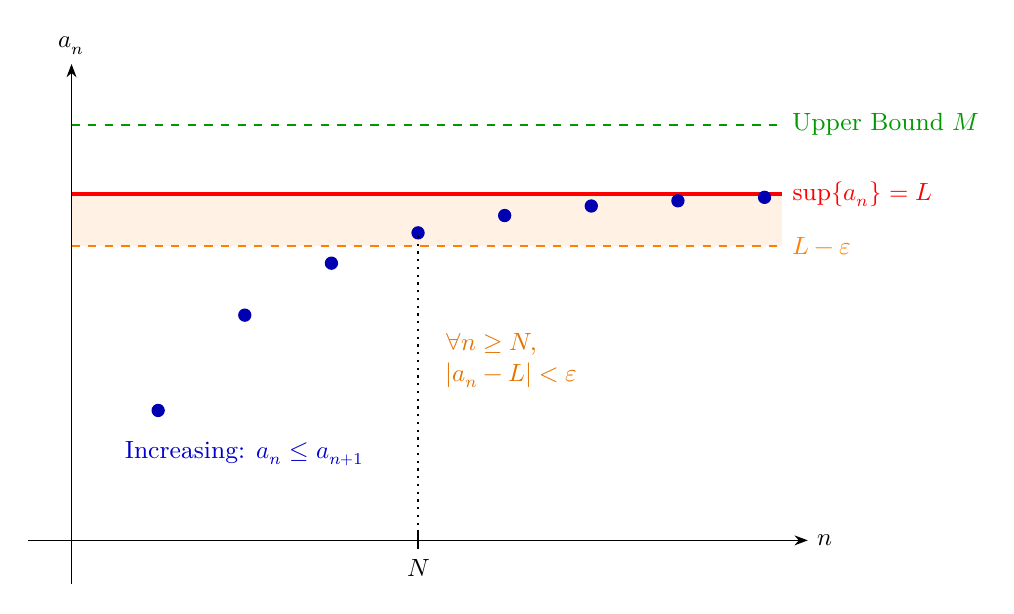
\begin{tikzpicture}[
                scale=1.1,
                >=Stealth, % 使用更好看的箭头
                font=\small
            ]
                % --- 定义参数 ---
                \def\Limit{4}      % 极限值 (Supremum)
                \def\Epsilon{0.6}  % Epsilon 大小
                \def\M{4.8}        % 普通上界

                % --- 坐标轴 ---
                \draw[->] (-0.5, 0) -- (8.5, 0) node[right] {$n$};
                \draw[->] (0, -0.5) -- (0, 5.5) node[above] {$a_n$};

                % --- 辅助区域 (Epsilon Strip) ---
                % 使用填充色展示 L - epsilon 到 L 之间的区域
                \fill[orange!10] (0, \Limit-\Epsilon) rectangle (8.2, \Limit);
                \draw[orange, dashed, thick] (0, \Limit-\Epsilon) -- (8.2, \Limit-\Epsilon) node[right] {$L - \varepsilon$};

                % --- 绘制线条 ---
                % 1. 普通上界 (Green)
                \draw[green!60!black, thick, dashed] (0, \M) -- (8.2, \M) node[right] {Upper Bound $M$};
                
                % 2. 上确界/极限 (Red)
                \draw[red, very thick] (0, \Limit) -- (8.2, \Limit) node[right] {$\sup\{a_n\} = L$};

                % --- 绘制数据点 (模拟单调递增数列) ---
                % 点坐标: (x, y)
                \coordinate (P1) at (1, 1.5);
                \coordinate (P2) at (2, 2.6);
                \coordinate (P3) at (3, 3.2);  % 还没进入 epsilon 区域
                \coordinate (P4) at (4, 3.55); % N点，刚好进入 (> 4-0.6=3.4)
                \coordinate (P5) at (5, 3.75);
                \coordinate (P6) at (6, 3.86);
                \coordinate (P7) at (7, 3.92);
                \coordinate (P8) at (8, 3.96);

                % 绘制点的循环
                \foreach \i in {1,...,8} {
                    \filldraw[blue!70!black] (P\i) circle (2pt);
                    % 可选：画垂线
                    %\draw[dotted, gray] (P\i) -- (\i, 0); 
                }

                % --- 标注 N (Critical Index) ---
                % 在 n=4 处
                \draw[dotted, thick] (4, 0) -- (4, 3.55);
                \draw[thick] (4, 0.1) -- (4, -0.1) node[below] {$N$};
                
                % --- 文字说明 ---
                % 说明 N 之后的点都在黄色区域内
                \node[text=orange!90!black, align=left, anchor=north west] at (4.2, 2.5) {
                    $\forall n \ge N$, \\
                    $|a_n - L| < \varepsilon$
                };
                
                % 说明单调性
                \node[text=blue!80!black] at (2, 1) {Increasing: $a_n \le a_{n+1}$};

            \end{tikzpicture}
            \caption{}
        \end{figure}

        The proof of another case is symmetric of above proof.

        \newpage

        \begin{example}[Recursive Radical Sequence]
        Consider the sequence defined by $a_1 = \sqrt{2}$ and $a_{n+1} = \sqrt{2 + a_n}$. Prove it converges and find the limit.

        \begin{proof}[Solution] We show the sequence satisfying the conditions of MCT.
            \begin{enumerate}
            \item \textbf{Boundedness:} We show $a_n$ bounded by induction.
            \begin{itemize}[itemsep=0.5em, topsep=0.5em]
                \item Base case: $a_1 = \sqrt{2} < 2$.
                \item Inductive step: Assume $a_k < 2$. Then $a_{k+1} = \sqrt{2+a_k} < \sqrt{2+2} = 2$.
            \end{itemize}
            Thus $\{a_n\}$ is bounded above by 2.

            \item \textbf{Monotonicity:} We show $a_{n+1} > a_n$.
            \[ a_{n+1} = \sqrt{2 + a_n} \implies a_{n+1}^2 - a_n^2 = 2 \implies a_{n+1} - a_n =\frac{2}{a_{n+1}+a_n} > 0 \]
            Since $0 < a_n < 2$, we have $(a_n - 2) < 0$ and $(a_n + 1) > 0$.
            Thus the sequence is increasing.

            \item \textbf{Limit:} By MST, the limit $L = \lim a_n$ exists.
            Taking the limit on both sides of $a_{n+1} = \sqrt{2 + a_n}$:
            \[ L = \sqrt{2 + L} \implies L^2 = 2 + L \implies L^2 - L - 2 = 0 \]
            Solutions are $L = 2$ or $L = -1$. Since $a_n > 0$, $L = 2$.
        \end{enumerate}
        \end{proof}
        \end{example}

        \begin{remark}
            留意本题中给出的数列是以递归关系给出的，即没有显式公式。
        \end{remark}

        \begin{remark}
            一般而言，有界性的证明依赖于数学归纳法。而单调性的证明有时需用数学归纳法，有时使用不等式的性质。
            核心思路是利用单调有界定理。
        \end{remark}

        \newpage

    \subsection{Subsequence}

        \begin{definition}[Subsequence]
        A \textbf{subsequence} of a sequence $\{a_n\}$ is a sequence $\{a_{n_k}\}$ where $\{n_k\}$ is a strictly increasing sequence of natural numbers:
        \[ n_1 < n_2 < n_3 < \dots \quad (n_k \in \mathbb{N}). \]
        \end{definition}

        \begin{remark}
            留意 $n_k \geq k$.
        \end{remark}

        \begin{theorem}[Subsequence Theorem / 子列定理]
        If a sequence $\{a_n\}$ converges to  $a$ and $\{a_{n_k}\}$ is a subsequence, then 
        % every subsequence $\{a_{n_k}\}$ of $\{a_n\}$ also converges to $a$.
        \[ \lim_{n \to \infty} a_n = a \implies \lim_{k \to \infty} a_{n_k} = a \]
        \end{theorem}

        \begin{proof}
        Let $\varepsilon > 0$. Since $a_n \to a$, there exists $N \in \mathbb{N}$ such that 
        $$\forall n \ge N, |a_n - a| < \varepsilon$$
        Since $\{n_k\}$ is strictly increasing integers, $n_k \ge k$.
        Therefore, for any $k \ge N$, we have $n_k \ge N$, which implies $|a_{n_k} - a| < \varepsilon$.
        \end{proof}

        \begin{remark}
            显然此定理的逆否形式说明若数列中存在两个收敛向不同值的子列，则该数列发散。例如
            $$
                a_{2k} \to L_1,\ a_{2k-1} \to L_2 \ \ \text{及}\ \ L_1 \neq L_2
            $$
            具体来说，取 $a_n = (-1)^n$，那么该数列的奇数项收敛到 $-1$ ，偶数项收敛到 $1$，显然该数列发散。
        \end{remark}

        \begin{theorem}[Intertwining Sequence Theorem / 奇偶子列定理]
        If the subsequence of even terms $\{a_{2n}\}$ and the subsequence of odd terms $\{a_{2n-1}\}$ 
        both converge to the same limit $a$, then the original sequence $\{a_n\}$ converges to $a$.
        $$
            \left( a_{2n} \to a \right) \land \left( a_{2n-1} \to a \right) \implies a_n \to a
        $$
        \end{theorem}

        \begin{proof}
        $\forall \varepsilon > 0$:
        \begin{align*}
            a_{2n} \to a &\implies \exists N_{even} \text{ s.t. } \forall n \ge N_{even}, |a_{2n} - a| < \varepsilon \\
            a_{2n-1} \to a &\implies \exists N_{odd} \text{ s.t. } \forall n \ge N_{odd}, |a_{2n-1} - a| < \varepsilon
        \end{align*}
        Let $N = \max\{2N_{even}, 2N_{odd}\}$. For any $k \ge N$:
        \begin{enumerate}
            \item If $k$ is even, $k/2 \ge N_{even} \implies |a_k - a| < \varepsilon$.
            \item If $k$ is odd, $(k+1)/2 \ge N_{odd} \implies |a_k - a| < \varepsilon$.
        \end{enumerate}
        Thus, $a_n \to a$.
        \end{proof}
        
        \newpage

        \begin{example}[Intertwining Recursive Sequence]
        Let $a_1 = 1$ and $a_{n+1} = \frac{1}{1 + a_n}$. Find the limit if it exists.
        \begin{proof}[Solution]
        Assuming convergence to $L$, limit laws give:
        \[ L = \frac{1}{1+L} \implies L(1+L) = 1 \implies L^2 + L - 1 = 0. \]
        Since $a_n > 0$, $L = \frac{-1 + \sqrt{5}}{2}$.

        To prove the limit exists, Consider $a_{2n}$ and $a_{2n-1}$, since
        $$a_{n+2} = \frac{1}{1 + \frac{1}{1+a_n}} = \frac{1+a_n}{2+a_n}<1$$
        are monotonic sequence. 
        So $a_{2n+2} = \frac{1+a_{2n}}{2+a_{2n}}$ and $a_{2n+1} = \frac{1+a_{2n-1}}{2+a_{2n-1}}$ 
        both monotonic and bounded.
        By MCT, $\{a_{2k}\}$ and $\{a_{2k-1}\}$ converges, clearly that $a_{2n},\ a_{2n+1}$ 
        converges to a same limit. Assume $a_{2n},\ a_{2n+1} \to L$ and take both limit, we have 
        $$L = \frac{1+L}{2+L}$$
        we have $L = \frac{-1 + \sqrt{5}}{2}$.
        By the \textbf{Intertwining Sequence Theorem}, the whole sequence converges.
        \end{proof}
        
        \end{example}

        \newpage

    \subsection{Nested Interval Theorem}

    \begin{theorem}[Nested Interval Theorem(区间套定理)]
    Let $\{I_n\}$ be a sequence of closed bounded intervals, where $I_n = [a_n, b_n]$. Suppose the intervals are nested, i.e.,
    \[ I_1 \supseteq I_2 \supseteq I_3 \supseteq \cdots \implies \forall n, [a_{n+1}, b_{n+1}] \subseteq [a_n, b_n]. \]
    Then the intersection is non-empty:
    \[ \bigcap_{n=1}^{\infty} I_n = [a, b] \]
    where $a = \lim_{n \to \infty} a_n$ and $b = \lim_{n \to \infty} b_n$.

    Furthermore, if $\lim_{n \to \infty} (b_n - a_n) = 0$, 
    then the intersection consists of exactly one point:
    \[ \bigcap_{n=1}^{\infty} I_n = \{x\} \]
    \end{theorem}

    \begin{proof}
    Since the intervals are nested ($I_{n+1} \subseteq I_n$), we have:
    \[ a_1 \le a_2 \le \cdots \le a_n \le a_{n+1} \le \cdots \le b_{n+1} \le b_n \le \cdots \le b_1. \]
    \begin{itemize}[itemsep = 0.5em, topsep = 0.5em]
        \item The sequence $\{a_n\}$ is increasing and bounded above by $b_1$.
        \item The sequence $\{b_n\}$ is decreasing and bounded below by $a_1$.
    \end{itemize}
    By the \textbf{Monotone Sequence Theorem}, both limits exist. Let $a = \lim a_n$ and $b = \lim b_n$.
    By limit inequality, since $a_n \le b_n$, we have $a \le b$.\\

    Now we prove $\bigcap_{n=1}^{\infty} I_n = [a, b]$.
    \begin{enumerate}
        \item For any $n$, since $\{a_k\}$ is increasing and $\{b_k\}$ is decreasing, 
        we have $$a_n \le a \le b \le b_n$$
        Thus, $[a, b] \subseteq [a_n, b_n] = I_n$ for all $n$. 
        \item If $x \in \bigcap I_n$, then $a_n \le x \le b_n$ for all $n$. 
            By Sandwich Theroem we get $x \in [a, b]$.
    \end{enumerate}
    $\implies \bigcap_{n=1}^{\infty} I_n = [a, b] $\\

    If $\lim (b_n - a_n) = 0$, then $b - a = 0 \implies a = b$. 
    The interval $[a, b]$ degenerates to the singleton set $\{a\}$.
    \end{proof}

    \begin{remark}
        事实上，区间套定理揭示了的定义实数的另一种方法，即利用单调序列构成的（长度）递减区间来唯一确定一个实数。
        由于有理数数列的极限不一定是有理数（其构造方法见波尔查诺-维尔斯特拉斯定理的证明细节），
        因此任意一个实数都可以透过构造有理数序列的方式进行逼近，结合区间套定理，我们可以确定唯一一个实数。
    \end{remark}

    \newpage

    \begin{figure}[htbp]
        \centering
        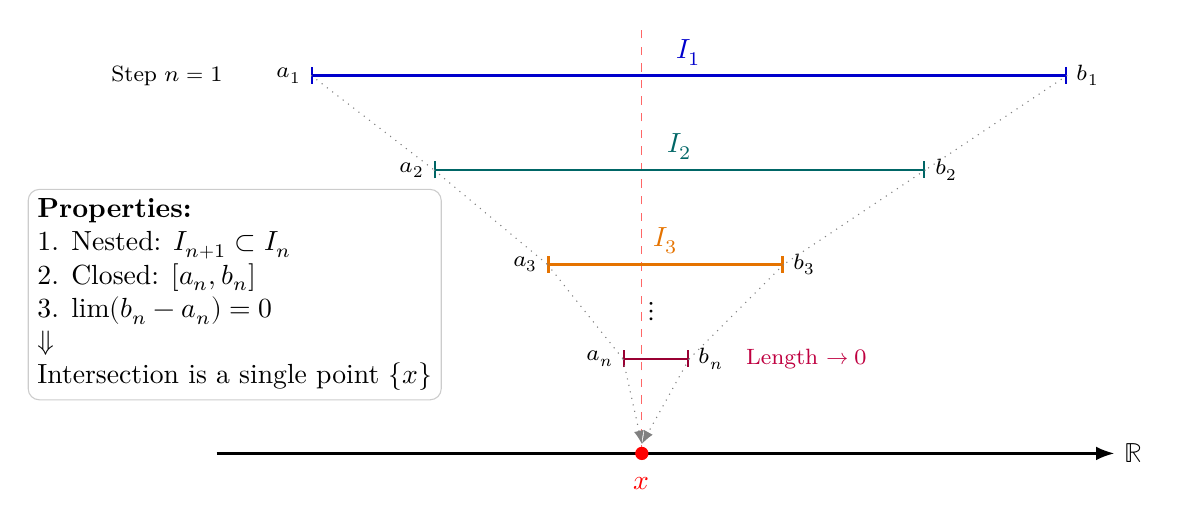
\begin{tikzpicture}[
            scale=1.2,
            >={Latex},
            interval/.style={thick, |-|}, % 区间样式：粗线，两端有垂直短线
            label_text/.style={font=\footnotesize}
        ]

            % ==========================
            % 定义参数
            % ==========================
            \def\Limit{4} % 极限点 x 的位置
            \def\YStart{4} % 第一层的高度
            \def\YStep{1.0} % 层间距

            % ==========================
            % 1. 绘制数轴 (最底层)
            % ==========================
            \draw[->, thick] (-0.5, 0) -- (9, 0) node[right] {$\mathbb{R}$};
            
            % 绘制极限点 x
            \fill[red] (\Limit, 0) circle (2pt) node[below=5pt, font=\bfseries] {$x$};
            
            % 绘制贯穿所有区间的虚线，强调 x 在所有区间内
            \draw[red, dashed, opacity=0.6] (\Limit, 0) -- (\Limit, \YStart + 0.5);

            % ==========================
            % 2. 绘制区间序列 (从上往下)
            % ==========================

            % --- Interval I_1 (n=1) ---
            \def\yOne{\YStart}
            \coordinate (A1) at (0.5, \yOne);
            \coordinate (B1) at (8.5, \yOne);
            
            \draw[interval, blue!80!black] (A1) -- (B1) node[midway, above] {$I_1$};
            \node[label_text, left] at (A1) {$a_1$};
            \node[label_text, right] at (B1) {$b_1$};
            \node[label_text, left=1cm] at (A1) {Step $n=1$};

            % --- Interval I_2 (n=2) ---
            \def\yTwo{\YStart - \YStep}
            \coordinate (A2) at (1.8, \yTwo);
            \coordinate (B2) at (7.0, \yTwo);
            
            \draw[interval, teal!80!black] (A2) -- (B2) node[midway, above] {$I_2$};
            \node[label_text, left] at (A2) {$a_2$};
            \node[label_text, right] at (B2) {$b_2$};
            
            % 绘制包含关系的视觉引导线 (灰色虚线)
            \draw[gray, dotted] (A1) -- (A2);
            \draw[gray, dotted] (B1) -- (B2);

            % --- Interval I_3 (n=3) ---
            \def\yThree{\YStart - 2*\YStep}
            \coordinate (A3) at (3.0, \yThree);
            \coordinate (B3) at (5.5, \yThree);
            
            \draw[interval, orange!90!black] (A3) -- (B3) node[midway, above] {$I_3$};
            \node[label_text, left] at (A3) {$a_3$};
            \node[label_text, right] at (B3) {$b_3$};
            
            \draw[gray, dotted] (A2) -- (A3);
            \draw[gray, dotted] (B2) -- (B3);

            % --- Interval I_k (Generic small interval) ---
            \def\yK{\YStart - 3*\YStep}
            \coordinate (Ak) at (3.8, \yK);
            \coordinate (Bk) at (4.5, \yK);
            
            % 省略号
            \node at (4.1, \yThree - 0.5*\YStep) {$\vdots$};
            
            \draw[interval, purple!80!black] (Ak) -- (Bk);
            \node[label_text, left] at (Ak) {$a_n$};
            \node[label_text, right] at (Bk) {$b_n$};
            \node[right, font=\footnotesize, purple] at (5.0, \yK) {Length $\to 0$};

            \draw[gray, dotted] (A3) -- (Ak);
            \draw[gray, dotted] (B3) -- (Bk);
            
            % 引导线指向极限点
            \draw[gray, ->, dotted] (Ak) -- (\Limit, 0.1);
            \draw[gray, ->, dotted] (Bk) -- (\Limit, 0.1);

            % ==========================
            % 3. 文字说明
            % ==========================
            \node[align=left, anchor=north west, draw=black!20, rounded corners] at (-2.5, 2.8) {
                \textbf{Properties:}\\
                1. Nested: $I_{n+1} \subset I_n$\\
                2. Closed: $[a_n, b_n]$\\
                3. $\lim (b_n - a_n) = 0$\\
                $\Downarrow$\\
                Intersection is a single point $\{x\}$
            };

        \end{tikzpicture}
        \caption{Visual demonstration of the Nested Interval Theorem. A sequence of closed ranges shrinking to a single point.}
    \end{figure}

    \subsection{Bolzano-Weierstrass Theorem in $\mathbb{R}$}

    This theorem is a powerful tool for proving convergence by extracting subsequences.

    \begin{theorem}[Bolzano-Weierstrass Theorem (波尔查诺-魏尔斯特拉斯定理)]
    Every bounded sequence $\{x_n\}$ of real numbers has a convergent subsequence.
    \end{theorem}

    \begin{proof}
    Since $\{x_n\}$ is bounded, there exist $A, B \in \mathbb{R}$ such that $\{x_n\} \subseteq [A, B]$. 
    Let $I_1 = [A, B]$.
    We construct a sequence of nested intervals $\{I_k\}$ using the \textbf{Method of Bisection}:

    \begin{enumerate}
        \item Divide $I_1$ into two equal closed subintervals. 
        At least one of these subintervals contain infinitely many terms of 
        the sequence $\{x_n\}$. Let $I_2$ be that interval.
        \item Repeat the process: Divide $I_k$ into two halves. Choose $I_{k+1}$ to be the half 
        containing infinitely many terms of $\{x_n\}$.
    \end{enumerate}

    By construction:
    \begin{enumerate}
        \item $I_1 \supseteq I_2 \supseteq I_3 \supseteq \cdots$.
        \item The length of $I_k$ is $|I_k| = \frac{B-A}{2^{k-1}}$. Thus $\lim_{k \to \infty} |I_k| = 0$.
    \end{enumerate}

    By the \textbf{Nested Interval Theorem}, $\bigcap_{k=1}^\infty I_k = \{x\}$ for some $x \in \mathbb{R}$.
    We now select terms $x_{n_k}$ to form the subsequence:
    \begin{enumerate}
        \item Pick $n_1 = 1$ such that $x_{n_1} \in I_1$.
        \item Since $I_2$ contains infinitely many terms, pick $n_2 > n_1$ such that $x_{n_2} \in I_2$.
        \item Generally, since $I_{k+1}$ contains infinitely many terms, choose $n_{k+1} > n_k$ such that $x_{n_{k+1}} \in I_{k+1}$.
    \end{enumerate}
    For this subsequence $\{x_{n_k}\}$, we have $x_{n_k} \in I_k$. Since $x \in I_k$ as well,
    \[ |x_{n_k} - x| \le \text{length}(I_k) = \frac{B-A}{2^{k-1}}. \]
    As $k \to \infty$, $\frac{B-A}{2^{k-1}} \to 0$. By the Sandwich Theorem, $\lim_{k \to \infty} x_{n_k} = x$.
    \end{proof}

    \newpage

    \subsection{Accumulation Points}

    The concept of an accumulation point (or limit point) generalizes the idea of limits to sets. The Bolzano-Weierstrass theorem can effectively be restated using this concept.

    \begin{definition}[Accumulation Point / 极限点]
    Let $S \subseteq \mathbb{R}$. A point $x \in \mathbb{R}$ is 
    called an \textbf{accumulation point} (or \textbf{limit point}) of $S$ 
    if every $\varepsilon$-neighborhood of $x$ contains at least one point of $S$ distinct from $x$.
    In logical symbols:
    \[ \forall \varepsilon > 0, \quad \left( (x - \varepsilon, x + \varepsilon) \cap S \right) \setminus \{x\} \neq \emptyset. \]
    \end{definition}

    \begin{remark}
        集合$S$的极限点不一定在$S$中，例如 $1$ 是 $S = (0,1)$ 的极限点，但 $1 \notin S$。
    \end{remark}

    \begin{theorem}
        If $x \in  \mathbb{R}$ is accumulation point of $S \subseteq \mathbb{R}$, then every
        $\varepsilon$-neighborhood of $x$ contains infinitely many points.
    \end{theorem}

    \begin{proof}
        
    \end{proof}

    \begin{theorem}
        If $x \in  \mathbb{R}$ is accumulation point of $S \subseteq \mathbb{R} \iff$ 
        there exists a sequence $\{s_n\}$ in $S \setminus \{x\}$ such that $$\lim_{n \to \infty} s_n = x$$
    \end{theorem}

    \begin{proof}[Sketch of proof]
        $(\Rightarrow)$ Take $\varepsilon = \frac{1}{n}$ in the definition of accumulation point 
        and choose $s_n \in (x-\frac{1}{n}, x+\frac{1}{n})\setminus \{x\}$ 
        for all $n$ to construct a sequence.\\

        $(\Leftarrow)$ Use the definition of convergence of sequence. 
    \end{proof}

    \begin{corollary}[Bolzano-Weierstrass Theorem for Sets]
    Every bounded, infinite subset of $\mathbb{R}$ has at least one accumulation point.
    \end{corollary}

    \newpage

    \subsection{Cauchy sequence}

    \begin{definition}[Cauchy Sequence / 柯西列]
    A sequence $\{a_n\}$ is called a \textbf{Cauchy sequence} if 
    \[ \forall \varepsilon > 0, \exists N \in \mathbb{N} \text{ such that } \forall m, n \ge N, \quad |a_m - a_n| < \varepsilon. \]
    \end{definition}

    \begin{theorem}[Convergence implies Cauchy]
    If a sequence $\{a_n\}$ converges, then $\{a_n\}$ is a Cauchy sequence.
    \end{theorem}

    \begin{proof}
    Let $\lim_{n \to \infty} a_n = a$. For any $\varepsilon > 0$, there exists $N \in \mathbb{N}$ such that $|a_k - a| < \frac{\varepsilon}{2}$ for all $k \ge N$.
    Then for any $m, n \ge N$, by the triangle inequality:
    \[ |a_m - a_n| = |(a_m - a) - (a_n - a)| \le |a_m - a| + |a_n - a| < \frac{\varepsilon}{2} + \frac{\varepsilon}{2} = \varepsilon. \]
    \end{proof}

    \begin{theorem}[Cauchy implies Boundedness]
    If $\{a_n\}$ is a Cauchy sequence, then $\{a_n\}$ is bounded (有界).
    \end{theorem}

    \begin{proof}
    Take $\varepsilon = 1$. By definition, $\exists N \in \mathbb{N}$ such that $\forall n \ge N$, $|a_n - a_N| < 1$, which implies $|a_n| < 1 + |a_N|$.
    Let $M = \max\{|a_1|, |a_2|, \dots, |a_{N-1}|, 1 + |a_N|\}$.
    Then $|a_n| \le M$ for all $n \in \mathbb{N}$.
    \end{proof}

    \subsection{Cauchy Convergence Criterion}

    This is a fundamental theorem in real analysis, stating that in $\mathbb{R}$, being Cauchy is equivalent to being convergent.

    \begin{theorem}[Cauchy's Criterion(柯西收敛准则)]
    A sequence $\{a_n\}$ of real numbers converges if and only if it is a Cauchy sequence.
    \end{theorem}

    \begin{proof}
    $(\implies)$ Already proved in Theorem 3.14.\\

    $(\impliedby)$ Suppose $\{a_n\}$ is a Cauchy sequence.
    \begin{enumerate}
        \item By Theorem 1.2, $\{a_n\}$ is bounded.
        \item By the \textbf{Bolzano-Weierstrass Theorem}, $\{a_n\}$ has a convergent subsequence $\{a_{n_k}\}$. Let $\lim_{k \to \infty} a_{n_k} = a$.
        \item We show the whole sequence converges to $a$.
        Since $\{a_n\}$ is Cauchy:
        \[ \forall \varepsilon > 0, \exists N_1 \text{ s.t. } \forall m, n \ge N_1, |a_m - a_n| < \frac{\varepsilon}{2}. \]
        Since $a_{n_k} \to a$:
        \[ \exists N_2 \text{ s.t. } \forall k \text{ with } n_k \ge N_2, |a_{n_k} - a| < \frac{\varepsilon}{2}. \]
        Let $N = \max(N_1, N_2)$. Fixed $n_k \ge N$. For any $n \ge N$:
        \[ |a_n - a| \le |a_n - a_{n_k}| + |a_{n_k} - a| < \frac{\varepsilon}{2} + \frac{\varepsilon}{2} = \varepsilon. \]
    \end{enumerate}
    Thus, $\lim_{n \to \infty} a_n = a$.
    \end{proof}

    \newpage

    \begin{example}
    Suppose a sequence $\{x_n\}$ is defined by the following recurrence relation:
    \[ x_1 = 0, \quad x_{n+1} = \frac{1}{4}(x_n^2 + 1) \quad \text{for any } n \in \mathbb{N}. \]

    \textbf{(a)} Prove that $0 \le x_n \le 1$ for all $n$, and prove there exists $c \in (0, 1)$ such that for any $n \ge 2$:
    \[ |x_{n+1} - x_n| \le c |x_n - x_{n-1}|. \]

    \textbf{(b)} Use Cauchy's theorem to show that $\{x_n\}$ converges.

    \begin{proof}[Solution (a):]
        We use induction.
        \begin{itemize}[itemsep = 0.5em, topsep = 0.5em]
            \item Base case: $x_1 = 0 \in [0, 1]$.
            \item Inductive step: Assume $0 \le x_k \le 1$. Then $x_{k+1} = \frac{1}{4}(x_k^2 + 1)$.
            Since $0 \le x_k^2 \le 1$, we have $1 \le x_k^2 + 1 \le 2$.
            Thus, $\frac{1}{4} \le x_{k+1} \le \frac{2}{4} = 0.5 < 1$.
        \end{itemize}
        So, $x_n \in [0, 1]$ for all $n$. And:
        \[
        \begin{aligned}
        |x_{n+1} - x_n| &= \left| \frac{1}{4}(x_n^2 + 1) - \frac{1}{4}(x_{n-1}^2 + 1) \right| \\
        &= \frac{1}{4} |x_n^2 - x_{n-1}^2| \\
        &= \frac{1}{4} |x_n + x_{n-1}| \cdot |x_n - x_{n-1}|.
        \end{aligned}
        \]
        Since $0 \le x_n \le 1$, we have $|x_n + x_{n-1}| \le 1 + 1 = 2$. Therefore:
        \[ |x_{n+1} - x_n| \le \frac{1}{4} \cdot 2 \cdot |x_n - x_{n-1}| = \frac{1}{2} |x_n - x_{n-1}|. \]
        Thus, the inequality holds with $c = \frac{1}{2} \in (0, 1)$.
    \end{proof}
    \begin{proof}[Solution (b):]
        By repeatedly applying the inequality from Part (a):
        \[ |x_{n+1} - x_n| \le c |x_n - x_{n-1}| \le c^2 |x_{n-1} - x_{n-2}| \le \cdots \le c^{n-1} |x_2 - x_1|. \]
        For any $m > n$, using the triangle inequality and geometric series sum:
        \[
        \begin{aligned}
        |x_m - x_n| &\le |x_m - x_{m-1}| + \cdots + |x_{n+1} - x_n| \\
        &\le (c^{m-2} + \cdots + c^{n-1}) |x_2 - x_1| \\
        &= c^{n-1} (1 + c + \cdots + c^{m-n-1}) |x_2 - x_1| \\
        &< c^{n-1} \left( \frac{1}{1-c} \right) |x_2 - x_1|.
        \end{aligned}
        \]
        Since $0 < c < 1$, $\lim_{n \to \infty} c^{n-1} = 0$.
        Thus, for any $\varepsilon > 0$, we can choose $N$  s.t 
        $$n > N > \log_c \left(\frac{\varepsilon (1-c)}{|x_2-x_1|}\right)+1$$
        We have $|x_m - x_n| < \varepsilon$. This proves $\{x_n\}$ is a Cauchy sequence. By \textbf{Cauchy's Theorem}, $\{x_n\}$ converges.
    \end{proof}
    \end{example}

    \newpage

    \section{Serise}

    \subsection{Definitions and Convergence}

    \begin{definition}[Infinite Series / 无穷级数]
    Let $\{a_k\}$ be a sequence of real numbers. An \textbf{infinite series} is an expression of the form:
    \[ \sum_{k=1}^{\infty} a_k = a_1 + a_2 + a_3 + \cdots \]
    \begin{enumerate}
        \item $a_k$ is called the $k^{th}$ \textbf{term} (项).
        \item $S_n = \sum_{k=1}^{n} a_k = a_1 + a_2 + \cdots + a_n$ is called the $n^{th}$ \textbf{partial sum} (部分和).
    \end{enumerate}
    \end{definition}

    \begin{definition}[Convergence / 收敛]
    A series $\sum_{k=1}^{\infty} a_k$ \textbf{converges} to a sum $S$ if and only if the sequence of partial sums $\{S_n\}$ converges to $S$.
    \[ \sum_{k=1}^{\infty} a_k = S \iff \lim_{n \to \infty} S_n = S. \]
    \begin{enumerate}
        \item If $\lim_{n \to \infty} S_n = \infty$ (or $-\infty$), the series \textbf{diverges to infinity} (发散至无穷).
        \item If $\lim_{n \to \infty} S_n$ does not exist, the series \textbf{diverges} (发散).
    \end{enumerate}
    \end{definition}

    \begin{remark}
        显然，部分和同样可以被视为数列。
        因此我们一样可以将无穷级数看成一种特殊的数列极限，即数列 $$S_n = \sum_{k=1}^{n}a_k$$ 的极限。
    \end{remark}

    \begin{example}
    \textbf{Geometric Series (几何级数):}
    Consider the series $\sum_{k=1}^{\infty} \frac{1}{2^{k-1}} = 1 + \frac{1}{2} + \frac{1}{4} + \cdots$.
    The partial sum is a geometric progression:
    \[ S_n = \frac{1 - (1/2)^n}{1 - 1/2} = 2 - \frac{1}{2^{n-1}}. \]
    Taking the limit:
    \[ \lim_{n \to \infty} S_n = \lim_{n \to \infty} \left( 2 - \frac{1}{2^{n-1}} \right) = 2. \]
    Thus, the series converges to 2.
    \end{example}

    \begin{example}
    \textbf{Divergent Series:}
    \begin{enumerate}
        \item Infinite sum of 1s: $\sum_{k=1}^{\infty} 1$. Since $S_n = n$, $\lim S_n = \infty$. The series diverges.
        \item Oscillating series: $\sum_{k=1}^{\infty} (-1)^{n-1} = 1 - 1 + 1 - \cdots$.
        \[ S_n = \begin{cases} 1 & \text{if } n \text{ is odd} \\ 0 & \text{if } n \text{ is even} \end{cases} \]
        The limit does not exist, so the series diverges.
    \end{enumerate}
    \end{example}

    \newpage

    \begin{example}
    \textbf{Famous Series:}
    \begin{enumerate}
        \item \textbf{Euler (Basel Problem):} $\displaystyle \sum_{k=1}^{\infty} \frac{1}{k^2} = \frac{\pi^2}{6}$.
        \item \textbf{Ramanujan:} A rapidly converging series for $\frac{1}{\pi}$:
        \[ \frac{2\sqrt{2}}{9801} \sum_{k=0}^{\infty} \frac{(4n)!(1103 + 26390n)}{(n!)^4 396^{4n}} = \frac{1}{\pi}. \]
    \end{enumerate}
    \end{example}

    \subsection{Algebra Properties}

    Let we denoted a notation:

    \begin{notation}
        $\sum a_n$ denoted an infinite series, i.e.
        $$
        \sum a_n = \sum_{n=1}^{\infty} a_n
        $$
    \end{notation}

    \begin{theorem}[Algebraic Properties]
    Let $\sum a_k$ and $\sum b_k$ be infinite series.

    \begin{enumerate}
        \item \textbf{Tail Invariance:} Convergence is determined by the "tail" of the series. For any $N \in \mathbb{N}$:
        \[ \sum_{k=1}^{\infty} a_k \text{ converges} \iff \sum_{k=N}^{\infty} a_k \text{ converges}. \]
        
        \item \textbf{Linearity:} If $\sum a_k = A$ and $\sum b_k = B$, then:
        \[ \sum_{k=1}^{\infty} (a_k \pm b_k) = A \pm B \]
        \[ \sum_{k=1}^{\infty} (c \cdot a_k) = c A \quad (\text{for any constant } c). \]
        
        \item \textbf{Non-negative Series:} If $a_k \ge 0$ for all $k$, then:
        \[ \sum_{k=1}^{\infty} a_k \text{ converges} \iff \text{Partial sums } \{S_n\} \text{ are bounded above}. \]
        I.e., $\exists M \in \mathbb{R}$ such that $S_n \le M$ for all $n$.
    \end{enumerate}
    \end{theorem}

    \begin{remark}
        这一部分的证明只利用基本的敛散性的定义即可轻易证明，
        由于先前说明过无穷级数的本质是数列的极限，因此不过多做证明。
    \end{remark}

    \newpage

    \section{Convergence Tests} 

    Let $\sum a_n$ be an infinite series. 
    The following tests are standard methods to determine whether the series converges or diverges.

    \begin{theorem}[Term Test / 项发散判别法]
        If $a_n \nrightarrow  0$, then 
        $
        \sum a_n
        $
        diverges. \\
        
        Note that if $\lim_{n \to \infty} a_n = 0$, 
        the test is \textbf{inconclusive} (the series may converge or diverge).
    \end{theorem}

    \begin{proof}
        We prove the contrapositive(逆否命题): Let $\sum a_n \to L$, then $\forall \varepsilon >0$, exists $N \in \mathbb{N}$ s.t
        $$
            \left| \sum_{k = 1}^{n}a_k - L \right| < {\varepsilon \over 2} ,\ \forall n \geq N
        $$
        Note that $a_{n+1} = \sum_{k = 1}^{n+1} a_k - \sum_{k = 1}^{n} a_k (n \geq r)$, so 
        $$
            |a_{n+1}| = \left| \sum_{k = 1}^{n+1} a_k -L +L - \sum_{k = 1}^{n} a_k \right| \leq 
            \left| \sum_{k = 1}^{n+1} a_k -L\right| + \left|\sum_{k = 1}^{n} a_k -L \right|
            < \frac{\varepsilon}{2}+\frac{\varepsilon}{2} = \varepsilon
        $$
        for all $n\geq N$.
    \end{proof}
    
        \begin{remark}
            留意这里我们选择 $|a_{n+1}|$ 而不是 $|a_n|$ 是因为这样可以避免出现 $\sum_{k = 1}^{n-1}a_k$ 导致我们无法使用定义。
        \end{remark}

    \begin{theorem}[Comparison Test / 比较判别法]
        Let $0 \le a_n \le b_n$.
        \begin{enumerate}
            \item If $\sum b_n$ converges $\implies \sum a_n$ converges.
            \item If $\sum a_n$ diverges $\implies \sum b_n$ diverges.
        \end{enumerate}
    \end{theorem}

    \begin{proof}
        Let $\sum b_n \to L \geq 0$, then the partial sums:
        $$
            B_n = \sum_{k = 1}^{n} b_r \geq \sum_{k = 1}^{n} a_r = A_n
        $$
        Since $B_n$ converges, so $B_n$ bounded, hence $A_n$ bounded. Clearly $A_n$ increasing, 
        by M.C.T. we have $A_n$ converges, i.e. $\sum a_n$ converges. 
    \end{proof}

    \begin{remark}
        两者互为逆否命题。
    \end{remark}

    \newcommand{\diffd}{\, \mathrm{d}}

    \begin{theorem}[Integral Test / 积分判别法]
        Let $f(x)$ be a continuous, positive, and decreasing function on $[1, \infty)$ such that $a_n = f(n)$.
        then 
        $$
        \int_1^{\infty} f(x) \diffd x \text{ converges} \iff \sum_{n=1}^{\infty} a_n \text{ converges}
        $$
    \end{theorem}

    \begin{proof}[Idea of proof]
        Use the follow inequality: (More details of proof see the appendix)
        $$
        \displaystyle \sum_{k=1}^{n} a_k \geq \int_{1}^{n} f(x) \diffd x \geq \sum_{k=2}^{n+1} a_k
        $$
    \end{proof}

    \begin{theorem}[Limit Comparison Test / 极限比较判别法]
        Let $a_n \geq 0, b_n > 0$. Define $L = \lim_{n \to \infty} \frac{a_n}{b_n}$. 
        \begin{enumerate}
            \item If $0 < L < \infty$, then $\sum a_n$ and $\sum b_n$ converge or diverge together.
            \item If $L = 0$ and $\sum b_n$ converges $\implies \sum a_n$ converges.
            \item If $L = \infty$ and $\sum b_n$ diverges $\implies \sum a_n$ diverges.
        \end{enumerate}
    \end{theorem}

    \begin{proof}
        By definition,, if $L \in [0,\infty)$, 
        then for all $\varepsilon>0$, exist $N \in \mathbb{N}$ s.t. $\forall n \geq N$ we have
        \begin{align*}
            &\left| \frac{a_n}{b_n} - L \right| < \varepsilon \\
            \iff &-\varepsilon <  \frac{a_n}{b_n} - L  < \varepsilon \\
            \iff &b_n \left( L - \varepsilon \right) <  a_n  < b_n \left( L + \varepsilon \right) 
        \end{align*}
        use comparison test we proved the first two case. If $L = \infty$, then 
        for all $r > 0$, exist $N \in \mathbb{N}$ s.t. $\forall n \geq N$ we have
        \begin{align*}
            \left| \frac{a_n}{b_n} \right| > r 
            \iff  a_n > r b_n
        \end{align*}
        use comparison test we proved the least case.
    \end{proof}

    \begin{theorem}[Alternating Series Test / Leibniz Test / 交错级数判别法] 

        Let infinite series $\sum (-1)^n b_n$ with $b_n > 0$. If
            \begin{enumerate}
                \item $b_n$ decreasing and
                \item $\lim_{n \to \infty} b_n = 0$.
            \end{enumerate}
            then $\sum (-1)^n b_n$ converges.
    \end{theorem}

    \begin{proof}
        Since $ b_n \to 0$ we have $\forall \varepsilon >0$, exist $N \in \mathbb{N}$ s.t 
        $$
            n \geq N \implies |b_n| < \varepsilon 
        $$
        $\forall m>n \geq \mathbb{N}$ we have:$$
        \begin{aligned}[t]
            \sum_{k=1}^{m} (-1)^k b_k - \sum_{k=1}^{n-1} (-1)^k b_k 
            &= (-1)^{n}\left( b_n -b_{n+1} + \cdots +(-1)^{m-n}b_{m} \right) \\
            \implies \left| \sum_{k=1}^{m} (-1)^k b_k - \sum_{k=1}^{n-1} (-1)^k b_k  \right| &= \left| b_n -b_{n+1} + \cdots +(-1)^{m-n}b_{m} \right| \\
            &\leq \left| b_n \right| (\text{Since the sequence is decreasing}) \\
            &< \varepsilon 
        \end{aligned}$$
        we have $S_n = \sum_{k=1}^{n} (-1)^k b_k$ form a Cauchy sequence. Hence 
        by Cauchy Theorem we have $\sum (-1)^n b_n$ converges.
    \end{proof}

    \newpage

    \begin{definition}[Convergent absolutely and Convergent conditionally / 绝对收敛与条件收敛]\quad
        \begin{enumerate}
            \item If $\sum |a_n|$ converges, the series is \textbf{convergent absolutely}.
            \item If $\sum a_n$ converges but $\sum |a_n|$ diverges, the series is \textbf{convergent conditionally}.
        \end{enumerate}

    \end{definition}

    \begin{theorem}[Absolute Convergence Test / 绝对收敛判别法]
        If $\sum |a_n|$ converges, then $\sum a_n$ converges.
    \end{theorem}

    \begin{proof}
        Use $-|a_n|\leq a_n \leq |a_n|$, we have $0 \leq a_n +|a_n| \leq 2|a_n|$. By comparison test we have 
        $\sum a_n$ converges.
    \end{proof}

    \begin{theorem}[Ratio Test / 比值判别法]
        Let $L = \lim_{n \to \infty} \left| \frac{a_{n+1}}{a_n} \right|$. We have
            \begin{enumerate}
                \item $L < 1 \implies \sum a_n$ absolutely convergent,
                \item $L > 1$ (or $\infty$) $\implies \sum a_n$ divergent,
                \item $L = 1 \implies$ the test \textbf{Inconclusive} (Try another test).
            \end{enumerate}
    \end{theorem}

    \begin{proof}
        Since $ \left| \frac{a_{n+1}}{a_n} \right| \to L$ we have $\forall \varepsilon >0$, exist $N \in \mathbb{N}$ 
        s.t $\forall  n \geq N$ we have$$
        \begin{array}{r c c c l}
            -\varepsilon &<& \left| \dfrac{a_{n+1}}{a_n} \right|  - L &<& \varepsilon \\
                    |a_n|(L-\varepsilon) &<& |a_{n+1}| &<& |a_n|(L + \varepsilon) \\
                    \vdots&\vdots&\vdots&\vdots&\vdots \\
                    |a_N|(L-\varepsilon)^{n-N+1} &<& |a_{n+1}| &<& |a_N|(L + \varepsilon)^{n-N+1} 
            
        \end{array}$$
        \begin{enumerate}
            \item If $L < 1$: Take $\varepsilon < 1-L$ we have $L + \varepsilon < 1$ and $\forall n \geq N$:
            $$\sum_{n\geq N} |a_{n+1}| < \sum_{n\geq N} |a_N|(L + \varepsilon)^n < \sum |a_N|(L + \varepsilon)^n $$
            \begin{remark}
                留意求和范围是对所有 $n \geq N$ 而非所有自然数 $n$, 因为上述的不等式关系只有当 $n \geq N$ 才生效。
                但由于$N$是固定常数，因此前$N$项和不影响敛散性。
            \end{remark}
            Note that $\sum |a_N|(L + \varepsilon)^n$ is a convergent geometry series. 
            By comparison test we have $\sum _{n\geq N}|a_{n+1}|$ converges, i.e. $\sum a_{n}$ 
            converges by absolute convergence test. 

            \item If $L > 1$:Take $\varepsilon < L - 1$ we have $1 < L - \varepsilon$ and $\forall n \geq N$:
            $$ |a_N|(L - \varepsilon)^{n-N+1} < |a_{n+1}| $$
            that implies $a_n \nrightarrow 0$, by term test we have $\sum a_n$ diverges.

            \item If $L = 1$: Consider $\sum_{n=1}^{\infty} \dfrac{1}{n}$ and $\sum_{n=1}^{\infty} \dfrac{1}{n^2}$
            , we have one diverges and another one converge.

            \item If $L = \infty$: We have $\forall r >0$, exist $N \in \mathbb{N}$ s.t 
            \begin{align*}
            n \geq N \implies&  \left| \frac{a_{n+1}}{a_n} \right| > r \\
            \implies&  \left| a_{n+1} \right| > |a_n| r > |a_N| r^{n-N+1} >0
            \end{align*}
            take $r = 1$ we have $a_n \nrightarrow 0$, 
            by term test we have $\sum a_n$ diverges.
        \end{enumerate}
    \end{proof}

    \newpage

    \begin{theorem}[Root Test / 根值判别法]
        Let $L = \lim_{n \to \infty} \sqrt[n]{|a_n|}$. We have
        \begin{enumerate}
            \item $L < 1 \implies \sum a_n $  absolutely convergent.
            \item $L > 1$ (or $\infty$) $\implies \sum a_n$ divergent.
            \item $L = 1 \implies$ the test \textbf{Inconclusive}.
        \end{enumerate}
    \end{theorem}

    \begin{proof}
        Since $ \sqrt[n]{|a_n|} \to L$ we have $\forall \varepsilon >0$, exist $N \in \mathbb{N}$ 
        s.t $\forall  n \geq N$ we have$$
        \begin{array}{r c c c l}
            -\varepsilon &<& \sqrt[n]{|a_n|}  - L &<& \varepsilon \\
                    L-\varepsilon &<& \sqrt[n]{|a_n|} &<& L + \varepsilon \\
                    (L-\varepsilon)^{n} &<& |a_n| &<& (L + \varepsilon)^{n} 
        \end{array}$$
        \begin{enumerate}
            \item If $L < 1$: Take $\varepsilon < 1-L$ 
            we have $L + \varepsilon < 1$ and $\forall n \geq N$:
            $$\sum_{n\geq N} |a_{n}| < \sum_{n\geq N} (L + \varepsilon)^n < \sum (L + \varepsilon)^n $$
            Note that $\sum (L + \varepsilon)^n$ is a convergent geometric series. 
            By comparison test we have $\sum _{n\geq N}|a_{n}|$ converges, i.e. $\sum a_{n}$ 
            converges by absolute convergence test. 

            \item If $L > 1$:Take $\varepsilon < L - 1$ we have $1 < L - \varepsilon$ and $\forall n \geq N$:
            $$ 1 < (L - \varepsilon)^{n} < |a_{n}| $$
            that implies $a_n \nrightarrow 0$, by term test we have $\sum a_n$ diverges.

            \item If $L = 1$: Consider $\sum_{n=1}^{\infty} \dfrac{1}{n}$ and $\sum_{n=1}^{\infty} \dfrac{1}{n^2}$
            , we have one diverges and another one converge.

            \begin{remark}
                We have $\dfrac{1}{\sqrt[n]{n}} \to 1$ see Example 3.2 .
                By the same reasons we have $\dfrac{1}{\sqrt[n]{n^2}} \to 1$.
            \end{remark}

            \item If $L = \infty$: We have $\forall r >0$, exist $N \in \mathbb{N}$ s.t 
            \begin{align*}
            n \geq N \implies&  \sqrt[n]{|a_n|} > r \\
            \implies&  |a_n| > r^n >0
            \end{align*}
            take $r = 1$ we have $a_n \nrightarrow 0$, 
            by term test we have $\sum a_n$ diverges.
        \end{enumerate}
    \end{proof}

    \newpage

    Moreover, use the Integral Test we have the follows corollary:

    \newcommand{\pseries}[1]{\mathcal{H}_{#1}}

    \begin{corollary}[p-test / p-级数判别法]
        Define the $p-\text{Series}$ as 
        $$
        \pseries{p} = \sum_{n=1}^{\infty} \dfrac{1}{n^p}
        $$
        where $p \in \mathbb{R}$. Then $\pseries{p}$ converges iff $p>1$.
    \end{corollary}

    Before introducing advanced tools, we review standard tests through examples.

    \begin{example}
    Consider the following series:
    \begin{enumerate}
        \item \textbf{Conditional Convergence:} 
        The harmonic series 
        $$\sum_{k=1}^\infty \frac{1}{k}$$
        diverges (Integral Test). 
        However, the alternating series 
        $$\sum_{k=1}^\infty (-1)^{k-1} \frac{1}{k}$$ 
        converges (Alternating Series Test).
        Thus, $\sum (-1)^{k-1} \frac{1}{k}$ converges conditionally.

        \item \textbf{Absolute Convergence:}
        Consider
        $$\sum_{k=1}^\infty \frac{\cos k}{k^2}$$ 
        Since $|\frac{\cos k}{k^2}| \le \frac{1}{k^2}$ and $\sum \frac{1}{k^2}$ converges (p-series, $p=2$), 
        the original series converges absolutely by the \textbf{Comparison Test}.

        \item \textbf{Limit Comparison Test:} Consider
        $$\sum_{k=2}^\infty \frac{\sqrt{k+1}}{k^2+5k}$$
        Compare with $b_k = \frac{\sqrt{k}}{k^2} = k^{-3/2}$.
        Since $\lim_{k \to \infty} \frac{a_k}{b_k} = 1$ and $\sum k^{-3/2}$ converges, the series converges.

        \item \textbf{Ratio Test:} Consider
        $$\sum_{k=1}^\infty \frac{k!}{k^k}$$
        Let $a_k = k!/k^k$, then
        \[ \lim_{k \to \infty} \left| \frac{a_{k+1}}{a_k} \right| = \lim_{k \to \infty} \frac{1}{(1 + \frac{1}{k})^k} = \frac{1}{e} < 1. \]
        Thus, the series converges.
    \end{enumerate}
    \end{example}

    \newpage

    % \section{Dirichlet's Test}

    \subsection{Summation by Parts}

    To handle more complicated series (like products of sequences), we need a discrete analogue to integration by parts.

    \begin{lemma}[Summation by Parts / Abe's Lemma]
    Let $\{a_k\}$ and $\{b_k\}$ be two sequences. Let 
    $$S_n = \sum_{k=1}^n a_k$$ 
    be the partial sum of $\{a_k\}$. 
    Define the forward difference $$\Delta b_k = b_{k+1} - b_k$$ 
    Then for any $n \ge 1$:
    \[ \sum_{k=1}^n a_k b_k = S_n b_n - \sum_{k=1}^{n-1} S_k \Delta b_k \]
    \end{lemma}

    \begin{proof}
    Let $S_0 = 0$. Since $a_k = S_k - S_{k-1}$, we have:
    \[
    \begin{aligned}
    \sum_{k=1}^n a_k b_k &= \sum_{k=1}^n (S_k - S_{k-1}) b_k \\
    &= (S_1 b_1 - S_0 b_1) + (S_2 b_2 - S_1 b_2) + \cdots + (S_n b_n - S_{n-1} b_n) \\
    &= S_n b_n + S_1(b_1 - b_2) + S_2(b_2 - b_3) + \cdots + S_{n-1}(b_{n-1} - b_n) \\
    &= S_n b_n - \left[ S_1(b_2 - b_1) + S_2(b_3 - b_2) + \cdots + S_{n-1}(b_n - b_{n-1}) \right] \\
    &= S_n b_n - \sum_{k=1}^{n-1} S_k (b_{k+1} - b_k).
    \end{aligned}
    \]
    \end{proof}

    \begin{remark}
        利用数列与级数的关键转换: $a_n = S_n - S_{n-1}$。
    \end{remark}

    \begin{remark}
        部分和事实上是分部积分在离散情况下的对应。
    \end{remark}

    \newpage

    \subsection{Dirichlet's Test}

    Dirichlet's test is a powerful tool, often generalizing the Alternating Series Test.

    \begin{theorem}[Dirichlet's Test / 狄利克雷判别法]
    Let $\sum_{k=1}^\infty a_k b_k$ be a series satisfying the following conditions:
    \begin{enumerate}
        \item The partial sums of $\{a_k\}$, denoted $S_n = \sum_{k=1}^n a_k$, form a \textbf{bounded sequence}. 
        % (i.e., $\exists M > 0$ such that $|S_n| \le M, \forall n$).
        \item The sequence $\{b_k\}$ is \textbf{decreasing} and 
        converges to 0.
        % (i.e., $b_k \ge b_{k+1}$ and $\lim_{k \to \infty} b_k = 0$).
    \end{enumerate}
    Then the series $\sum_{k=1}^\infty a_k b_k$ converges.
    \end{theorem}

    \begin{proof}
    Using Summation by Parts formula for partial sums:
    \[ \sum_{k=1}^n a_k b_k = S_n b_n - \sum_{k=1}^{n-1} S_k (b_{k+1} - b_k) \]
    We consider the two terms on the RHS as $n \to \infty$:
    \begin{enumerate}
        \item Since $\{S_n\}$ is bounded ($|S_n| \le M$) ，we have $-Mb_n \leq S_n b_n \leq M b_n$, 
        by the Sandwich Theorem, $\lim_{n \to \infty} S_n b_n = 0$.
        \item Consider the sum $\displaystyle\sum_{1 \leq k \leq n-1} S_k(b_{k+1}-b_k)$. Since $b_n \to 0$ and decreasing, 
        so $b_n \geq 0$, we have
        \[
        b_{k+1} - b_k < b_1 - b_k < b_1
        \]
        Hence we have: 
        \[
        \sum_{k=1}^{n-1} S_k (b_{k+1} - b_k) \leq \sum_{k=1}^{n-1} |S_k| |b_{k+1} - b_k|
        \leq \sum_{k=1}^{n-1} M (b_k - b_{k+1}) = M (b_1 - b_n ) \to M b_1 
        \]
        So $\displaystyle\sum_{1\leq k \leq n-1} |S_k| |b_{k+1} - b_k|$ is bounded and increasing, By M.C.T. 
        we have there are converges.
        \begin{remark}
            注意 $\displaystyle\sum_{1\leq k \leq n-1} |S_k| |b_{k+1} - b_k|$ 是正项级数，必定单调递增。
            前面关于级数的代数性质的定理中也提到：正向级数收敛当且仅当其有界。
        \end{remark}
        By the \textbf{Absolute Convergence Test}, $\sum S_k \Delta b_k$ converges.
    \end{enumerate}
    Therefore, $\lim_{n \to \infty} \sum_{k=1}^n a_k b_k$ exists.
    \end{proof}

    \begin{remark}
        该证明的关键是利用部分和公式将原级数的部分和啊拆成两项分别独立分析他们的敛散性。
    \end{remark}

    \begin{remark}
        交错级数判别法是狄利克雷判别法取 $a_k = (-1)^k$ 的一个特例.
    \end{remark}

    \begin{remark}
        事实上，将数列 $b_k$ 的条件从单调递减更变为单调，则该判别法依旧成立。
        更一般的，只需保证 $\sum \Delta b_n$ 收敛与 $b_n \to 0$ 即可。
    \end{remark}

    \newpage

    \begin{example}
    Show that $\displaystyle \sum_{k=1}^\infty \frac{\sin k}{k}$ converges.

    \begin{analysis}
        Standard tests (Ratio, Root, Absolute) fail. We use Dirichlet's Test.
    Let $a_k = \sin k$ and $b_k = \frac{1}{k}$.
    \end{analysis}
    \begin{proof}
        \begin{enumerate}
            \item \textbf{Check $b_k$:} $\{1/k\}$ is clearly decreasing and $\lim_{k \to \infty} \frac{1}{k} = 0$.
            \item \textbf{Check $a_k$ (Boundedness of Partial Sums):}
            We need to show $S_n = \sum_{k=1}^n \sin k$ is bounded. We use the trigonometric identity:
            \[ \sin m \sin \frac{1}{2} = \frac{1}{2} \left( \cos(m - \frac{1}{2}) - \cos(m + \frac{1}{2}) \right) \]
            Summing from $m=1$ to $n$:
            \[ S_n \sin \frac{1}{2} = \sum_{k=1}^n \sin k \sin \frac{1}{2} = \frac{1}{2} \left( \cos \frac{1}{2} - \cos(n + \frac{1}{2}) \right) \]
            \[ \implies S_n = \frac{\cos(1/2) - \cos(n + 1/2)}{2 \sin(1/2)} \]
            Since $|\cos x| \le 1$, the numerator is bounded by 2. Thus:
            \[ |S_n| \le \frac{2}{2 |\sin(1/2)|} = \frac{1}{\sin(1/2)} \]
            So $\{S_n\}$ is a bounded sequence.
        \end{enumerate}
        By Dirichlet's Test, $\displaystyle\sum \frac{\sin k}{k}$ converges.
    \end{proof}
    \end{example}

    

    Following the discussion on Dirichlet's Test and the series $\sum \frac{\sin k}{k}$:

    \begin{remark}
    \begin{enumerate}
        \item \textbf{Exact Value:} By using advanced techniques (such as Fourier Series), it can be shown that:
        \[ \sum_{k=1}^{\infty} \frac{\sin k}{k} = \frac{\pi - 1}{2}. \]
        
        \item \textbf{Conditional Convergence:} It can be proved that the series converges only conditionally. That is:
        \[ \sum_{k=1}^{\infty} \left| \frac{\sin k}{k} \right| \quad \text{diverges}. \]
    \end{enumerate}
    \end{remark}
    
    \newpage

    \section{The Cauchy Product}

    \subsection{Definition}

    \begin{definition}[Cauchy Product / 柯西乘积]
    Given two series $\sum_{k=0}^{\infty} a_k$ and $\sum_{k=0}^{\infty} b_k$, we define their \textbf{Cauchy product} to be the series $\sum_{k=0}^{\infty} c_k$, where the terms $c_k$ are defined by the convolution formula:
    \[ c_k = \sum_{i=0}^{k} a_i b_{k-i} = a_0 b_k + a_1 b_{k-1} + \cdots + a_k b_0. \]
    \end{definition}

    \begin{remark}
        在这里，我们不关心给定两个级数的敛散性。事实上，柯西乘积是有限求和乘积的推广。
    \end{remark}

    \begin{remark}
        若我们定义 $c_{i,j} = a_i b_j$，则
        $$
            \sum_{k=0}^{n} a_k \sum_{k=0}^{n} b_k = 
            \begin{array}{ c c c c c c c c c}
                c_{0,0} &+& c_{0,1} &+& c_{0,2} &+& \cdots &+& c_{0,n} + \\
                c_{1,0} &+& c_{1,1} &+& c_{1,2} &+& \cdots &+& c_{1,n} + \\
                c_{2,0} &+& c_{2,1} &+& c_{2,2} &+& \cdots &+& c_{2,n} + \\
                \vdots & \vdots & \vdots & \vdots & \vdots & \vdots & \vdots & \vdots &\\
                c_{n,0} &+& c_{n,1} &+& c_{n,2} &+& \cdots &+& c_{n,n}  \\
            \end{array} 
        $$
        可以发现：
        $$
            \sum_{k=0}^{n} a_k \sum_{k=0}^{n} b_k 
            = \sum^{n}_{k=0}c_k + \sum^{n}_{k = 1} \sum^{k-1}_{j = 0} a_k b_{n-j}
        $$
        可以发现右方第一项是柯西乘积的部分和，右方第二项是下三角部分（不包括对角线）的和，
        因此两级数部分和的乘积并不等于柯西乘积。
        但当 $n \to \infty$ 时，下三角部分不会被“取到”，这给予了在无穷下定义乘积的合理性。

    \end{remark}

    \subsection{Mertens' Theorem}

    \begin{theorem}[Mertens' Theorem]
    Suppose $\sum_{k=0}^{\infty} a_k$ converges \textbf{absolutely} to $A$, and $\sum_{k=0}^{\infty} b_k$ converges to $B$. Then their Cauchy product $\sum_{k=0}^{\infty} c_k$ converges to $AB$.
    \[ \left( \sum_{k=0}^{\infty} a_k = A \right) \land \left( \sum_{k=0}^{\infty} b_k = B \right) \implies \sum_{k=0}^{\infty} c_k = AB. \]
    \end{theorem}

    % \begin{proof}
    % Define the partial sums:
    % \[ A_n = \sum_{k=0}^n a_k, \quad B_n = \sum_{k=0}^n b_k, \quad C_n = \sum_{k=0}^n c_k. \]
    % Let $\beta_n = B_n - B$. Since $B_n \to B$, we have $\lim_{n \to \infty} \beta_n = 0$.

    % First, we express $C_n$ in terms of $A_n$ and $B_n$.
    % \[
    % \begin{aligned}
    % C_n &= c_0 + c_1 + \cdots + c_n \\
    % &= a_0 b_0 + (a_0 b_1 + a_1 b_0) + \cdots + (a_0 b_n + \cdots + a_n b_0) \\
    % &= a_0 (b_0 + \cdots + b_n) + a_1 (b_0 + \cdots + b_{n-1}) + \cdots + a_n b_0 \\
    % &= a_0 B_n + a_1 B_{n-1} + \cdots + a_n B_0 \\
    % &= a_0 (B + \beta_n) + a_1 (B + \beta_{n-1}) + \cdots + a_n (B + \beta_0) \\
    % &= B(a_0 + \cdots + a_n) + (a_0 \beta_n + a_1 \beta_{n-1} + \cdots + a_n \beta_0) \\
    % &= A_n B + \gamma_n,
    % \end{aligned}
    % \]
    % where $\gamma_n = \sum_{k=0}^n a_k \beta_{n-k}$.

    % Since $\lim_{n \to \infty} A_n = A$, we have $\lim_{n \to \infty} A_n B = AB$. To prove $C_n \to AB$, it suffices to show that $\lim_{n \to \infty} \gamma_n = 0$.

    % \textbf{Estimating $\gamma_n$:}
    % \begin{enumerate}
    %     \item Let $K = \sum_{k=0}^{\infty} |a_k|$. Note that $K$ exists because $\sum a_k$ converges absolutely.
    %     \item Since $B_n \to B$, the sequence $\{\beta_n\}$ converges to 0 and is bounded. Let $M > 0$ be a bound such that $|\beta_n| \le M$ for all $n$.
    %     \item For any $\varepsilon > 0$:
    %     \begin{itemize}
    %         \item Since $\beta_n \to 0$, $\exists N_1$ such that $|\beta_n| < \frac{\varepsilon}{2K}$ for all $n > N_1$.
    %         \item Since $\sum |a_k|$ converges, the tail sum vanishes. $\exists N_2$ such that $\sum_{k=N_2+1}^{\infty} |a_k| < \frac{\varepsilon}{2M}$.
    %     \end{itemize}
    %     Let $N = \max(N_1, N_2)$. Consider any $m > 2N$. We split the sum $\gamma_m$:
    %     \[
    %     \begin{aligned}
    %     |\gamma_m| &= \left| \sum_{k=0}^m a_k \beta_{m-k} \right| \le \sum_{k=0}^m |a_k| |\beta_{m-k}| \\
    %     &= \sum_{k=0}^N |a_k| |\beta_{m-k}| + \sum_{k=N+1}^m |a_k| |\beta_{m-k}|.
    %     \end{aligned}
    %     \]
    %     \begin{itemize}
    %         \item \textbf{First part:} Since $k \le N$ and $m > 2N$, the index $m-k > N$. Thus $|\beta_{m-k}| < \frac{\varepsilon}{2K}$.
    %         \[ \sum_{k=0}^N |a_k| |\beta_{m-k}| < \frac{\varepsilon}{2K} \sum_{k=0}^N |a_k| \le \frac{\varepsilon}{2K} \cdot K = \frac{\varepsilon}{2}. \]
    %         \item \textbf{Second part:} We use the bound $|\beta_{m-k}| \le M$.
    %         \[ \sum_{k=N+1}^m |a_k| |\beta_{m-k}| \le M \sum_{k=N+1}^m |a_k| < M \cdot \frac{\varepsilon}{2M} = \frac{\varepsilon}{2}. \]
    %     \end{itemize}
    %     Combining these, $|\gamma_m| < \frac{\varepsilon}{2} + \frac{\varepsilon}{2} = \varepsilon$.
    % \end{enumerate}
    % Thus, $\lim_{n \to \infty} \gamma_n = 0$, which implies $\lim_{n \to \infty} C_n = AB$.
    % \end{proof}

    \begin{remark}
    绝对收敛性是必要的。考虑
    $$a_k = b_k = \frac{(-1)^k}{\sqrt{k+1}}$$
    两者对应的级数均条件收敛。但两者的柯西乘积通项：
    \[ c_n = \sum_{k=0}^n a_k b_{n-k} = \sum_{k=0}^n \frac{(-1)^k}{\sqrt{k+1}} \cdot \frac{(-1)^{n-k}}{\sqrt{n-k+1}} = (-1)^n \sum_{k=0}^n \frac{1}{\sqrt{(k+1)(n-k+1)}}. \]
    对应的级数是：
    \[ |c_n| = \sum_{k=0}^n \frac{1}{\sqrt{(k+1)(n-k+1)}} \ge \sum_{k=0}^n \frac{1}{n+1} = \frac{n+1}{n+1} = 1. \]
    因为 $\lim_{n \to \infty} c_n \neq 0$, 根据项发散测试有 $\sum c_n$ 发散。
    \end{remark}

    \newpage

    \chapter{Limit and Continuity}

    \section{Limits of Functions}

    \subsection{Definition}

    \begin{definition}[Limit of a Function]

    Let $f: S \to \mathbb{R}$ be a function, and let $x_0$ be an \textbf{accumulation point} of $S$.

    We say that $f(x)$ \textbf{converges} to $L$ as $x$ tends to $x_0$, 
    denoted by $$\lim_{x \to x_0} f(x) = L$$ if and only if:
    \[
    \forall \varepsilon > 0, \exists \delta > 0 \text{ such that } \forall x \in S, \quad 0 < |x - x_0| < \delta \implies |f(x) - L| < \varepsilon.
    \]
    % If $f(x)$ not converges as $x \to x_0$, then we say the limit of $f(x)$ as $x \to x_0$ does not exist.
    \end{definition}

    \begin{remark}
        \begin{enumerate}
            \item $f(x)$ 在 $x=x_0$ 处的极限不要求 $x_0 \in \domain f$。只需 $f$ 在 $x_0$ 附近的开邻域内有定义。
            \item $f(x)$ 在 $x=x_0$ 处的极限是唯一的。证明参照数列极限唯一性的证明。
        \end{enumerate}
    \end{remark}

    \begin{example}
    Consider the function $f(x) = x \sin\left(\frac{1}{x}\right)$ for $x \neq 0$. 
    Prove that $$\lim_{x \to 0} f(x) = 0$$

    \begin{proof}
        $\forall \varepsilon > 0, \exists \delta > 0$ s.t. $0 < |x| < \delta \implies |f(x)| < \varepsilon$.
        Observe that:
        \[
        |f(x) - 0| = \left| x \sin\left(\frac{1}{x}\right) \right| 
        = |x| \cdot \left| \sin\left(\frac{1}{x}\right) \right| \leq |x|
        \]
    
        For any given $\varepsilon > 0$, choosing $\delta = \varepsilon$ we have:
        \[
        0 < |x| < \delta \implies |f(x)| \le |x| < \delta = \varepsilon
        \]
        Thus, $\displaystyle\lim_{x \to 0} f(x) = 0$.
    \end{proof}
    \end{example}

    \newpage

    \subsection{Properties of limit of functions}

    \begin{theorem}[Sequential Limit Theorem / 海涅定理]
    Let $f: S \to \mathbb{R}$. Then
    \[ \lim_{x \to x_0} f(x) = L \]
    if and only if for every sequence $\{x_n\} \subseteq S \setminus \{x_0\}$ converging to $x_0$, the sequence $\{f(x_n)\}$ converges to $L$.
    \[ \lim_{x \to x_0} f(x) = L \iff \left( \forall \{x_n\} \to x_0 \text{ ($x_n \neq x_0$)}, \lim_{n \to \infty} f(x_n) = L \right). \]
    \end{theorem}

    \begin{proof}
    ($\implies$):
    Suppose $\displaystyle\lim_{x \to x_0} f(x) = L$. Let $\{x_n\}$ 
    be any sequence in $S \setminus \{x_0\}$ such that $x_n \to x_0$. By definition:
    $$
        \forall \varepsilon > 0, \exists \delta > 0 ,\ 0 < |x - x_0| < \delta \implies |f(x) - L| < \varepsilon
    $$
    Since $x_n \to x_0$, we have for this specific $\delta$:
    $$
        \exists N \in \mathbb{N} ,\ \forall n \ge N, |x_n - x_0| < \delta
    $$
    Combining both we have $\exists N \in \mathbb{N}, \forall n \ge N$, $0 < |x_n - x_0| < \delta \implies |f(x_n) - L| < \varepsilon$. 
    Thus we have $$\lim_{n \to \infty} f(x_n) = L$$

    ($\impliedby$):
    We prove by contradiction.
    Suppose $\lim_{x \to x_0} f(x) \neq L$ (or the limit does not exist).
    Then take the negation:
    \[ \exists \varepsilon_0 > 0\ \text{ such that }\ \forall \delta > 0, 
    \exists x \in S\ \text{ s.t. }\ 0 < |x - x_0| < \delta \text{ but } |f(x) - L| \ge \varepsilon_0 \]
    For each $n \in \mathbb{N}$, let $\delta_n = \frac{1}{n}$. From the negation above, there exists $x_n \in S$ such that:
    \[ 0 < |x_n - x_0| < \frac{1}{n} \quad \text{and} \quad |f(x_n) - L| \ge \varepsilon_0 \]
    From $0 < |x_n - x_0| < \frac{1}{n}$, 
    by the Sandwich Theorem, $\displaystyle\lim_{n \to \infty} x_n = x_0$. 
    But $|f(x_n) - L| \ge \varepsilon_0$ implies ${f(x_n)  \nrightarrow L}$. 
    This contradicts the assumption that $x_n \to x_0 \implies f(x_n) \to L$. Therefore, $\displaystyle\lim_{x \to x_0} f(x)$ must be $L$.
    \end{proof}

    \begin{remark}
        第一部分的证明比较简单。第二部分的证明思路是透过在反证法下构造序列制造矛盾，
        思路是透过 $0 < |x - x_0| < \delta$ 观察到其与数列极限的定义相似，于是尝试构造特殊的序列 $\delta_n$ 
        并使用夹逼定理构造矛盾。
    \end{remark}

    \begin{remark}
        该定理表明 $\displaystyle\lim_{n \to \infty} f(x_n) = f(\lim_{n \to \infty} x_n)$
    \end{remark}

    \newpage

    \begin{example}
    Using the $\varepsilon$-definition of the limit, prove that:
    \[ \lim_{x \to 1} \frac{3x}{x^2+2} = 1 \]

    \begin{analysis}
        We want to show that 
        \begin{center}
            $\forall \varepsilon > 0$, 
            exist $\delta > 0$ s.t. $|x-1|<\delta \implies |f(x) - 1|<\varepsilon$
        \end{center}
        Let's simplify the expression $|f(x) - L|$:
        $$
        \begin{aligned}
        \left| \frac{3x}{x^2+2} - 1 \right| 
        &= \left| \frac{3x - (x^2+2)}{x^2+2} \right| 
        = \left| \frac{-(x-1)(x-2)}{x^2+2} \right| \\
        &= |x-1| \cdot \frac{|x-2|}{x^2+2} \\
        & \leq |x-1| \cdot \frac{|x-2|}{2} 
        \end{aligned}
        $$
        Set $\delta \leq 1$, then $0<x<2$, we have $\frac{|x-2|}{2} < 1$.
    \end{analysis}

    \begin{proof}
        By above analysis, we have
        $$
            |f(x) - 1| < |x-1| < \delta
        $$
        $\forall \varepsilon > 0$, 
        set $(\delta \leq \varepsilon) \land (\delta \leq 1)$, i.e. $\delta = \min(1,\varepsilon)$, 
        we have $|f(x) - 1| < \varepsilon$.
    \end{proof}

    \end{example}

    \begin{example}[Disproving Limits using Sequences]
    Prove that the limit does not exist:
    \[ \lim_{x \to 2} \sin \left( \frac{1}{x-2} \right) \]

    \begin{proof}
        We use the \textbf{Sequential Limit Theorem}:

        \textbf{Sequence 1:} Choose $x_n$ such that $\sin(\dots) = 1$.
        We set $\frac{1}{x_n - 2} = 2n\pi + \frac{\pi}{2}$. Solving for $x_n$:
        \[ x_n - 2 = \frac{1}{2n\pi + \pi/2} \implies x_n = 2 + \frac{1}{2n\pi + \pi/2} \]
        As $n \to \infty$, the denominator goes to infinity, so $x_n \to 2$.
        The function value is:
        \[ f(x_n) = \sin \left( 2n\pi + \frac{\pi}{2} \right) = 1 \implies \lim_{n \to \infty} f(x_n) = 1 \]

        \textbf{Sequence 2:} Choose $y_n$ such that $\sin(\dots) = 0$.
        We set $\frac{1}{y_n - 2} = n\pi$. Solving for $y_n$:
        \[ y_n - 2 = \frac{1}{n\pi} \implies y_n = 2 + \frac{1}{n\pi} \]
        As $n \to \infty$, $y_n \to 2$.
        The function value is:
        \[ f(y_n) = \sin(n\pi) = 0 \implies \lim_{n \to \infty} f(y_n) = 0 \]

        So the limit $\lim_{x \to 2} \sin \left( \frac{1}{x-2} \right)$ does not exist.
    \end{proof}
    \end{example}

    \newpage

    \begin{theorem}[Algebraic Limit Theorem / 极限的四则运算]
    Suppose $f, g: S \to \mathbb{R}$ are functions. Let $\lim_{x \to x_0} f(x) = L_1$ and $\lim_{x \to x_0} g(x) = L_2$. Then:

    \begin{enumerate}
        \item \textbf{Sum/Difference:} 
        \[ \lim_{x \to x_0} (f(x) \pm g(x)) = L_1 \pm L_2 \]
        
        \item \textbf{Product:} 
        \[ \lim_{x \to x_0} (f(x) g(x)) = L_1 L_2 \]
        
        \item \textbf{Quotient:} 
        \[ \lim_{x \to x_0} \frac{f(x)}{g(x)} = \frac{L_1}{L_2}, \quad \text{provided } g(x) \neq 0 \text{ for } x \in S \setminus \{x_0\} \text{ and } L_2 \neq 0 \]
    \end{enumerate}
    \end{theorem}

    \begin{proof}[Sketch of Proof]
    We utilize the \textbf{Sequential Limit Theorem} .
    Let $\{x_n\}$ be any sequence in $S \setminus \{x_0\}$ such that $x_n \to x_0$.
    By the assumption, we know that the image sequences converge:
    \[ f(x_n) \to L_1 \quad \text{and} \quad g(x_n) \to L_2 \quad \text{as } n \to \infty. \]
    Using the algebraic limit theorems for \textit{sequences}:
    \begin{enumerate}
        \item $(f+g)(x_n) = f(x_n) + g(x_n) \to L_1 + L_2$.
        \item $(fg)(x_n) = f(x_n)g(x_n) \to L_1 L_2$.
        \item $(f/g)(x_n) = f(x_n)/g(x_n) \to L_1/L_2$ (since $L_2 \neq 0$).
    \end{enumerate}
    Since this holds for \textit{any} sequence $x_n \to x_0$, the function limits must be $L_1 \pm L_2$, $L_1 L_2$, and $L_1/L_2$ respectively.
    \end{proof}

    \begin{remark}
        海涅定理可以将函数的极限问题转化为数列的极限问题。
    \end{remark}

    \begin{theorem}[Sandwich Theorem / 夹逼定理]
    Suppose $f, g, h$ are real-valued functions on $S$. If there exists an open interval $I$ containing $x_0$ such that:
    \[ f(x) \ge g(x) \ge h(x) \quad \forall x \in I \setminus \{x_0\} \subseteq S \]
    and
    \[ \lim_{x \to x_0} f(x) = L \quad \text{and} \quad \lim_{x \to x_0} h(x) = L \]
    then
    \[ \lim_{x \to x_0} g(x) = L \]
    \end{theorem}

    \begin{proof}[Sketch of Proof]
    Let $\{x_n\} \subset I \setminus \{x_0\}$ be any sequence converging to $x_0$.
    By the hypothesis, we have the inequality for sequences:
    \[ f(x_n) \ge g(x_n) \ge h(x_n) \]
    Since $f(x_n) \to L$ and $h(x_n) \to L$, by the \textbf{Sandwich Theorem for Sequences}, we must have $g(x_n) \to L$.
    By the Sequential Limit Theorem, this implies $\lim_{x \to x_0} g(x) = L$.
    \end{proof}

    \newpage

    \begin{theorem}[Limit Inequality / 极限的保序性]
    Suppose $f, g$ are real-valued functions on $S$. If there exists an open interval $I$ containing $x_0$ such that:
    \[ f(x) \ge g(x) \quad \forall x \in I \setminus \{x_0\} \subseteq S \]
    and the limits exist:
    \[ \lim_{x \to x_0} f(x) = L \quad \text{and} \quad \lim_{x \to x_0} g(x) = M, \]
    then $L \ge M$.
    \end{theorem}

    \begin{proof}[Sketch of Proof]
    Take any sequence $x_n \to x_0$. Since $f(x_n) \ge g(x_n)$ for all $n$, 
    the Limit Inequalitie for sequences guarantees that $\lim f(x_n) \ge \lim g(x_n)$, 
    which means $L \ge M$.
    \end{proof}

    \subsection{One-Side Limit}

    \begin{definition}[One-Sided Limits]
    Let $f: (a, b) \to \mathbb{R}$ and $x_0 \in (a, b)$.

    \begin{enumerate}
        \item \textbf{Left-hand limit (左极限):} $f(x_0-) = \lim_{x \to x_0^-} f(x) = L$ iff:
        \[ \forall \varepsilon > 0, \exists \delta > 0 \text{ s.t. } \forall x \in (a, b), \quad 0 < x_0 - x < \delta \implies |f(x) - L| < \varepsilon \]
        
        \item \textbf{Right-hand limit (右极限):} $f(x_0+) = \lim_{x \to x_0^+} f(x) = L$ iff:
        \[ \forall \varepsilon > 0, \exists \delta > 0 \text{ s.t. } \forall x \in (a, b), \quad 0 < x - x_0 < \delta \implies |f(x) - L| < \varepsilon \]
    \end{enumerate}
    \end{definition}

    \begin{corollary}[Relationship to Limits]
    The limit exists if and only if both one-sided limits exist and are equal:
    \[ \lim_{x \to x_0} f(x) = L \iff f(x_0-) = L = f(x_0+) \]
    \end{corollary}

    \begin{remark}
    Most standard limit theorems (Algebraic Limit Theorem, Sandwich Theorem, Limit Inequality) also hold for limits at infinity.
    \end{remark}

    \begin{example}
    Consider the function $f(x) = \frac{|x|}{x}$ for $x \neq 0$. 
    Prove that:
    \[ \lim_{x \to 0^+} f(x) = 1 \]

    \begin{proof}
        \textbf{ Right-hand limit:}
        We want to show $\lim_{x \to 0^+} f(x) = 1$.
        By definition, we need to show:
        \[ \forall \varepsilon > 0, \exists \delta > 0 \text{ s.t. } 0 < x < \delta \implies |f(x) - 1| < \varepsilon. \]
        Let $\varepsilon > 0$ be arbitrary.
        Since $x > 0$, we have $f(x) = \frac{x}{x} = 1$.
        Substituting this into the inequality:
        \[ |f(x) - 1| = |1 - 1| = 0 \]
        Since $0 < \varepsilon$ is always true for any positive $\varepsilon$, 
        the condition holds for any $\delta > 0$.
        We can simply choose $\delta = 1$ (or any positive number).
        Thus, if $0 < x < \delta$, then $|f(x) - 1| = 0 < \varepsilon$.
        So, $\displaystyle\lim_{x \to 0^+} f(x) = 1$.
    \end{proof}
    \begin{remark}
        同样的方法，我们有 $\displaystyle \lim_{x \to x_0^-} f(x) = -1$。
        由此，根据推论 4.1 有 $\displaystyle\lim_{x \to 0} f(x)$ 不
    \end{remark}

    \end{example}


    \newpage

    \begin{definition}[Monotone Functions]
    Let $f: S \to \mathbb{R}$. For any $x, y \in S$ with $x < y$:
    \begin{enumerate}
        \item \textbf{Increasing (单调递增):} $f(x) \le f(y)$.
        \item \textbf{Strictly increasing (严格递增):} $f(x) < f(y)$.
        \item \textbf{Decreasing (单调递减):} $f(x) \ge f(y)$.
        \item \textbf{Strictly decreasing (严格递减):} $f(x) > f(y)$.
    \end{enumerate}
    The function $f$ is called \textbf{monotone} if it is either increasing or decreasing.
    \end{definition}

    \begin{example}[Analysis of Monotonicity]
    Determine the monotonicity of the following functions on the given intervals:
    \begin{enumerate}
        \item $f(x) = x^3$ on $\mathbb{R}$.
        \item $g(x) = \frac{1}{x}$ on $(0, \infty)$.
    \end{enumerate}

    \begin{proof}[Solution]\quad
        \begin{enumerate}
        \item For $f(x) = x^3$:
        Let $x_1, x_2 \in \mathbb{R}$ with $x_1 < x_2$.
        Since the cube function preserves order:
        \[ x_1 < x_2 \implies x_1^3 < x_2^3 \implies f(x_1) < f(x_2). \]
        Thus, $f$ is \textbf{strictly increasing (严格递增)} on $\mathbb{R}$.

        \item For $g(x) = \frac{1}{x}$:
        Let $x_1, x_2 \in (0, \infty)$ with $x_1 < x_2$.
        Taking reciprocals reverses the inequality for positive numbers:
        \[ 0 < x_1 < x_2 \implies \frac{1}{x_1} > \frac{1}{x_2} \implies g(x_1) > g(x_2). \]
        Thus, $g$ is \textbf{strictly decreasing (严格递减)} on $(0, \infty)$.

    \end{enumerate}
    \end{proof}
    \end{example}

    \begin{definition}[Boundedness]
    Let $S_0 \subseteq S$. The function $f$ is:
    \begin{enumerate}
        \item \textbf{Bounded above (上界):} if $\{f(x) \mid x \in S_0\}$ is bounded above.
        \item \textbf{Bounded below (下界):} if $\{f(x) \mid x \in S_0\}$ is bounded below.
        \item \textbf{Bounded (有界):} if it is both bounded above and below.
    \end{enumerate}
    \end{definition}

    \begin{example}
    Check if $f(x) = \frac{x}{x+1}$ is bounded on the interval $S = [0, \infty)$.

    \begin{proof}[Solution]
        We need to check if the set $\{ f(x) \mid x \in S \}$ is bounded.
        \begin{enumerate}
        \item \textbf{Lower Bound:} Since $x \ge 0$, we have $x+1 > 0$, thus $f(x) \ge 0$.
        \item \textbf{Upper Bound:} For $x \ge 0$:
        \[ f(x) = \frac{x}{x+1} = \frac{x+1-1}{x+1} = 1 - \frac{1}{x+1}. \]
        Since $\frac{1}{x+1} > 0$, we have $f(x) < 1$.
    \end{enumerate}
    Since $0 \le f(x) < 1$ for all $x \in S$, $f$ is \textbf{bounded (有界)} on $[0, \infty)$.
    \end{proof}
    \end{example}

    \newpage

    \subsection{Monotone Function Theorem}

    Monotone functions behave very nicely regarding limits: limits always exist (possibly infinite), and discontinuities are simple "jumps".

    \begin{theorem}[Monotone Function Theorem]
    If $f$ is \textbf{increasing} on $(a, b)$, then for any $x_0 \in (a, b)$, the one-sided limits exist and satisfy:
    \[ f(x_0-) = \sup \{ f(x) \mid a < x < x_0 \} \quad \text{and} \quad f(x_0+) = \inf \{ f(x) \mid x_0 < x < b \}. \]
    Furthermore:
    \begin{enumerate}
        \item If $f$ is bounded below, $f(a+)$ exists.
        \item If $f$ is bounded above, $f(b-)$ exists.
        \item The set of discontinuities $J = \{ x_0 \in (a, b) \mid f(x_0-) \neq f(x_0+) \}$ is \textbf{countable} (at most countably many jump discontinuities).
    \end{enumerate}
    \end{theorem}

    \begin{proof}
    Since $f$ is increasing, the set $A = \{ f(x) \mid a < x < x_0 \}$ is bounded above by $f(x_0)$. By the Completeness Axiom, let $M = \sup A$.
    For any $\varepsilon > 0$, there exists $c \in (a, x_0)$ such that 
    $$M - \varepsilon < f(c) \le M$$
    Tkae $ c < x < x_0$, we have $0 < x-c <x_0 - c$. Let $\delta = x_0 - c$, we have
    \[ f(c) \le f(x) \le M \implies M - \varepsilon < f(x) \le M \implies |f(x) - M| < \varepsilon. \]
    Thus, $f(x_0-) = M$. The proof for $f(x_0+)$ is similar using infimum.\\
    
    If $x_0 \in J$, then $f(x_0-) < f(x_0+)$. By the density of rational numbers $\mathbb{Q}$, there exists a rational number $q(x_0) \in \mathbb{Q}$ such that:
    \[ f(x_0-) < q(x_0) < f(x_0+). \]
    For distinct points $x_0 < x_1$, we have $f(x_0+) \le f(x_1-)$, so the intervals $(f(x_0-), f(x_0+))$ and $(f(x_1-), f(x_1+))$ are disjoint. Hence $q(x_0) \neq q(x_1)$.
    This defines an injection from $J$ to $\mathbb{Q}$. Since $\mathbb{Q}$ is countable, $J$ is countable.
    \end{proof}

    \begin{remark}
        透过交换 $\sup, \inf$ 我们可以得出函数在递减时的情况。
    \end{remark}

    \begin{center}
    \begin{tikzpicture}[scale=1.5]
        % Axes
        \draw[->] (-0.5,0) -- (5,0) node[right] {$x$};
        \draw[->] (0,-0.5) -- (0,4) node[above] {$y$};

        % Coordinates for the jump
        \def\xZero{2.5}
        \def\yLeft{1.5}
        \def\yRight{2.5}

        % Left part of the curve (increasing)
        \draw[thick, blue] (0.5, 0.5) to[out=20, in=200] (\xZero, \yLeft);
        \draw[fill=white, draw=blue] (\xZero, \yLeft) circle (1.5pt); % Open circle for limit

        % Right part of the curve (increasing)
        \draw[thick, blue] (\xZero, \yRight) to[out=20, in=200] (4.5, 3.5);
        \draw[fill=blue, draw=blue] (\xZero, \yRight) circle (1.5pt); % Closed circle (assuming right continuous or just defined there)

        % Labels on axes
        \draw[dashed] (\xZero, 0) -- (\xZero, \yRight);
        \node[below] at (\xZero, 0) {$x_0$};

        \draw[dashed] (0, \yLeft) -- (\xZero, \yLeft);
        \node[left] at (0, \yLeft) {$f(x_0-) = \sup \{f(x) : x < x_0\}$};

        \draw[dashed] (0, \yRight) -- (\xZero, \yRight);
        \node[left] at (0, \yRight) {$f(x_0+) = \inf \{f(x) : x > x_0\}$};

        % Highlighting the jump
        \draw[<->, red] (\xZero+0.1, \yLeft) -- (\xZero+0.1, \yRight);
        \node[right, red, align=left] at (\xZero+0.1, {(\yLeft+\yRight)/2}) {Jump\\Gap};

        % Interval notation
        \node[below] at (0.5, 0) {$a$};
        \node[below] at (4.5, 0) {$b$};
    \end{tikzpicture}
    \end{center}

    \newpage

    \subsection{Divergence and Infinite Limit}

    \begin{remark}
        本篇章主要涵盖3种情况下的极限：
        \begin{enumerate}
            \item （在某处发散至无穷）$x \to x_0$ 时 $f(x) \to \infty$。
            \item （在无穷远处收敛）$x \to \infty$ 时 $f(x) \to L \in \mathbb{R}$。
            \item （在无穷远处发散至无穷）$x \to \infty$ 时 $f(x) \to \infty$。
        \end{enumerate}
    \end{remark}

    \begin{definition}[Infinite Limits / 发散至无穷]
    Let $f: S \to \mathbb{R}$ be a function and $x_0$ be an accumulation point.
    \begin{enumerate}
        \item We say $f$ \textbf{diverges to $\infty$} (or has limit $\infty$) as $x$ tends to $x_0$ (denoted $\lim_{x \to x_0} f(x) = \infty$) if and only if:
        \[ \forall r \in \mathbb{R}, \exists \delta > 0 \text{ such that } 0 < |x - x_0| < \delta \implies f(x) > r. \]
        
        \item Similarly, $f$ \textbf{diverges to $-\infty$} (denoted $\lim_{x \to x_0} f(x) = -\infty$) if and only if:
        \[ \forall r \in \mathbb{R}, \exists \delta > 0 \text{ such that } 0 < |x - x_0| < \delta \implies f(x) < r. \]
    \end{enumerate}
    \end{definition}

    \begin{remark}
    The one-sided infinite limits (e.g., $\lim_{x \to x_0^+} f(x) = \infty$) can be similarly defined by restricting the domain to $x > x_0$ or $x < x_0$.
    \end{remark}

    \begin{definition}[Convergent Limits at Infinity / 无穷远处收敛]
    Let $f: S \to \mathbb{R}$. Suppose $\infty$ (or $-\infty$) is an accumulation point of $S$ (i.e., there is a sequence in $S$ diverging to $\infty$ or $-\infty$).

    \begin{enumerate}
        \item We say $f(x)$ \textbf{converges to $L$} as $x \to \infty$ (denoted $\lim_{x \to \infty} f(x) = L$) iff:
        \[ \forall \varepsilon > 0, \exists K \in \mathbb{R} \text{ such that } \forall x \in S, \quad x \ge K \implies |f(x) - L| < \varepsilon. \]
        
        \item We say $f(x)$ \textbf{converges to $L$} as $x \to -\infty$ (denoted $\lim_{x \to -\infty} f(x) = L$) iff:
        \[ \forall \varepsilon > 0, \exists K \in \mathbb{R} \text{ such that } \forall x \in S, \quad x \le K \implies |f(x) - L| < \varepsilon. \]
    \end{enumerate}
    \end{definition}

    \begin{remark}
    Most standard limit theorems (Algebraic Limit Theorem, Sandwich Theorem, Limit Inequality) also hold for limits at infinity.
    \end{remark}

    \begin{definition}[Divergent Limits at Infinity / 无穷远处的无穷极限]
    Let $f: S \to \mathbb{R}$.
    \begin{enumerate}
        \item $\lim_{x \to \infty} f(x) = \infty$ (or $-\infty$) iff:
        \[ \forall r \in \mathbb{R}, \exists K \in \mathbb{R} \text{ such that } x \ge K \implies f(x) > r \quad (\text{or } f(x) < r). \]
        
        \item $\lim_{x \to -\infty} f(x) = \infty$ (or $-\infty$) iff:
        \[ \forall r \in \mathbb{R}, \exists K \in \mathbb{R} \text{ such that } x \le K \implies f(x) > r \quad (\text{or } f(x) < r). \]
    \end{enumerate}
    \end{definition}

    \newpage

    \begin{example}[Polynomial Growth]
    For $n \in \mathbb{N}$, let $p(x) = a_n x^n + a_{n-1} x^{n-1} + \dots + a_0$ be an $n$-th degree polynomial. Suppose $a_n > 0$. Then:
    \[ \lim_{x \to \infty} p(x) = \infty. \]

    \noindent \textbf{Proof Sketch:}
    We use the inequality technique to bound the lower-order terms.
    \[
    \begin{aligned}
    p(x) &\ge a_n x^n - |a_{n-1}|x^{n-1} - \dots - |a_0| \\
    &\ge a_n x^n - (|a_{n-1}| + \dots + |a_0|) x^{n-1} \quad (\text{for } x > 1).
    \end{aligned}
    \]
    We want to show this is greater than any $r$.
    We can choose $x$ large enough such that the leading term dominates. Specifically, if we ensure:
    \[ p(x) \ge \frac{1}{2} a_n x^n + \left[ \frac{1}{2} a_n x^n - (|a_{n-1}| + \dots + |a_0|) x^{n-1} \right]. \]
    If the term in the brackets is non-negative, then $p(x) \ge \frac{1}{2} a_n x^n$.
    This leads to the choice of $K$:
    \[ K = \max \left\{ \frac{2(|a_{n-1}| + \dots + |a_0|)}{a_n}, \left( \frac{2r}{a_n} \right)^{\frac{1}{n}} \right\} + 1. \]
    Then for $x \ge K$, $p(x) > r$.
    Similarly, if $a_n < 0$, then $\lim_{x \to \infty} p(x) = -\infty$.
    \end{example}

    \begin{example}[Reciprocals]
    Using the result above, if $p(x)$ is a polynomial of degree $n \ge 1$, then:
    \[ \lim_{x \to \infty} \frac{1}{p(x)} = 0. \]
    More generally, if $\lim_{x \to \infty} f(x) = \pm \infty$, then $\lim_{x \to \infty} \frac{1}{f(x)} = 0$.
    \end{example}

    \begin{example}[Two-sided Check]
    Consider $f(x) = 1/x$.
    \[ \lim_{x \to 0^+} \frac{1}{x} = \infty \quad \text{and} \quad \lim_{x \to 0^-} \frac{1}{x} = -\infty. \]
    Since the limits are not the same (one is $+\infty$, one is $-\infty$), 
    we cannot simply say $\lim_{x \to 0} \frac{1}{x} = \infty$ or $-\infty$. 
    The limit does not exist in $\mathbb{R}$ by corollary 4.1 .
    \end{example}

    \newpage

    \section{Continuity}

    \begin{definition}[Continuity at a Point / 于某点处连续]
    A function $f: S \to \mathbb{R}$ is \textbf{continuous} (连续) at $x_0 \in S$ if and only if:
    \[ \lim_{x \to x_0} f(x) = f(x_0) \]
    In terms of $\varepsilon-\delta$ notation:
    \[ \forall \varepsilon > 0, \exists \delta > 0 \text{ such that } \forall x \in S, \quad |x - x_0| < \delta \implies |f(x) - f(x_0)| < \varepsilon \]
    \end{definition}

    \begin{definition}[Continuity on a Set]
    For a subset $E \subseteq S$:
    \begin{enumerate}
        \item $f$ is continuous on $E$ iff $f$ is continuous at all points $x \in E$.
        \item $f$ is simply called \textbf{continuous} if it is continuous on its entire domain $S$.
    \end{enumerate}
    \end{definition}

    This theorem bridges the gap between the limit of a function and the limit of sequences, simplifying many proofs.

    \begin{theorem}[Sequential Continuity Theorem]
    $f: S \to \mathbb{R}$ is continuous at $x_0 \in S$ if and only if for any sequence $\{x_n\}$ in $S$:
    \[ \lim_{n \to \infty} x_n = x_0 \implies \lim_{n \to \infty} f(x_n) = f(x_0). \]
    \end{theorem}
    \begin{remark}
        只需将海涅定理中的 $L$ 替换成 $x_0$ 即可。
    \end{remark}

    \begin{example}[Dirichlet Function / 狄利克雷函数]
    Consider the function $f: \mathbb{R} \to \mathbb{R}$ defined by:
    \[
    f(x) = \begin{cases} 
    1 & \text{if } x \in \mathbb{Q} \quad (\text{Rational}) \\
    0 & \text{if } x \notin \mathbb{Q} \quad (\text{Irrational})
    \end{cases}
    \]
    Then $f$ is not continuous at any point in $\mathbb{R}$.

    \begin{proof}
    Let $x_0 \in \mathbb{R}$ be arbitrary.
    By the \textbf{density} of rational and irrational numbers, for any $n \in \mathbb{N}$, we can find:
    \[ r_n \in \mathbb{Q} \quad \text{and} \quad s_n \in \mathbb{R} \setminus \mathbb{Q} \]
    such that both fall within the interval $(x_0 - \frac{1}{n}, x_0)$. That is:
    \[ x_0 - \frac{1}{n} < r_n < x_0 \quad \text{and} \quad x_0 - \frac{1}{n} < s_n < x_0. \]
    By the Sandwich Theorem, as $n \to \infty$:
    \[ \lim_{n \to \infty} r_n = x_0 \quad \text{and} \quad \lim_{n \to \infty} s_n = x_0. \]
    However, evaluating the function limits:
    \[ \lim_{n \to \infty} f(r_n) = \lim_{n \to \infty} 1 = 1 \quad \text{and} \quad \lim_{n \to \infty} f(s_n) = \lim_{n \to \infty} 0 = 0. \]
    Since the limits of the image sequences are different ($1 \neq 0$), $\lim_{x \to x_0} f(x)$ does not exist. Thus, $f$ is discontinuous at $x_0$.
    \end{proof}
    \end{example}

    \newpage

    \subsection{Some properties}

    \begin{theorem}[Algebraic Properties]
    If $f, g: S \to \mathbb{R}$ are continuous at $x_0 \in S$, then the following functions are also continuous at $x_0$:
    \begin{enumerate}
        \item $f \pm g$
        \item $f \cdot g$
        \item $f / g$ \quad (provided $g(x_0) \neq 0$)
    \end{enumerate}
    \end{theorem}

    \begin{theorem}[Continuity of Composition / 复合函数的连续性]
    Let $f: S \to \mathbb{R}$ and $g: S' \to \mathbb{R}$ be functions such that the range $f(S) \subseteq S'$.
    If:
    \begin{enumerate}
        \item $f$ is continuous at $x_0$, and
        \item $g$ is continuous at $y_0 = f(x_0)$,
    \end{enumerate}
    then the composite function $g \circ f$ is continuous at $x_0$.

    \end{theorem}

    \begin{proof}
    We use the Sequential Continuity Theorem,
    %  for any sequence $x_n \to x_0$ in $S$, $\lim (g \circ f)(x_n) = (g \circ f)(x_0)$.
    \begin{enumerate}
        \item Since $f$ is continuous at $x_0$ and $x_n \to x_0$, we have $f(x_n) \to f(x_0)$.
        \item Let $y_n = f(x_n)$ and $y_0 = f(x_0)$. Then $y_n \to y_0$.
        \item Since $g$ is continuous at $y_0$, we have $g(y_n) \to g(y_0)$.
    \end{enumerate}
    Substituting back, $g(f(x_n)) \to g(f(x_0))$. Thus, $g \circ f$ is continuous at $x_0$.
    \end{proof}

    
    The Sign Preserving Property intuitively states that continuous functions cannot change their 
    sign abruptly.

    \begin{theorem}[Sign Preserving Property / 保号性]
    Let $g: S \to \mathbb{R}$ be a continuous function at $x_0 \in S$, where $S$ is an interval with positive length.
    If $g(x_0) > 0$, then there exists a neighborhood $(x_0 - \delta, x_0 + \delta)$ such that:
    \[ \forall x \in S \cap (x_0 - \delta, x_0 + \delta), \quad g(x) > 0. \]
    (Similarly, if $g(x_0) < 0$, then $g(x)$ remains negative in a neighborhood of $x_0$.)
    \end{theorem}

    \begin{proof}
    Let $\varepsilon = g(x_0)$. Since $g(x_0) > 0$, we have $\varepsilon > 0$.
    By the definition of continuity at $x_0$, there exists $\delta > 0$ such that for all $x \in S$:
    \[ |x - x_0| < \delta \implies |g(x) - g(x_0)| < \varepsilon \]
    Expanding the inequality $|g(x) - g(x_0)| < g(x_0)$:
    \[ -g(x_0) < g(x) - g(x_0) < g(x_0) \]
    Focusing on the left side:
    \[ g(x) > g(x_0) - g(x_0) = 0 \]
    Thus, $g(x) > 0$ for all $x$ in the $\delta$-neighborhood.
    \end{proof}
    
    \begin{remark}
        这个性质说明了每一个连续函数在取值非零的“附近”总会保持相同的符号。
    \end{remark}

    % \begin{remark}
    % 这个定理的直观解释如下：如果函数 $f$ 的图像是连续不断的（unbroken），且图像上的某一点 $(x_0, g(x_0))$ 位于 $x$ 轴上方，那么该点及其附近的图像部分也一定位于 $x$ 轴上方。这也意味着函数值的正负号在局部是保持不变的。
    % \end{remark}

    \newpage

    \subsection{Extreme and Intermediate Value Theorem}

    \subsubsection{Boundary and EVT}

    \begin{theorem}
        If $f : [a,b] \to \mathbb{R}$ be a continuous function. Then $f$ bounded.
    \end{theorem}

    \begin{proof}
        Suppose $f$ not bounded. Then $\forall n \in \mathbb{N}$ 
        there exist $x_n \in [a,b]$ s.t. 
        $$
        \begin{aligned}
            \left| f(x_n) \right| > n
        \end{aligned}
        $$
        By Bolzano-Weierstrass Theorem, 
        exist $\{ x_{n_k} \} \subseteq \{ x_n \}$ s.t. $x_{n_k} \to x_0$ 
        for some $x_0 \in [a,b]$. Since $f$ continuous, 
        so $\forall x_{n_k} \to x_0$, $f(x_{n_k}) \to f(x_0) \in \mathbb{R}$. But 
        $$
            \left| f(x_{n_k}) \right| > n_k > n \to \infty
        $$
        Then we have a contradiction.
    \end{proof}

    \begin{remark}
        即闭区间上的连续 $\implies$ 有界。
    \end{remark}

    \begin{theorem}[Extreme Value Theorem / EVT]
        If $f : [a,b] \to \mathbb{R}$ be a continuous function. Then exists $m, M \in [a,b]$ s.t.
        $$
            f(m) = \inf_{x \in [a,b]} f(x) \quad \quad f(M) = \sup_{x \in [a,b]} f(x)
        $$
    \end{theorem}

    \begin{proof}
        Suppose for all $x \in [a,b]$, $f(x) < \sup_{x \in [a,b]} f(x) =S$. Consider
        $$
            g(x) = \dfrac{1}{S - f(x)}
        $$
        we have $g$ is also continuous and by \textbf{Supremum property}:
        $$
        S-\varepsilon < f(x) \leq S
        $$
        for all $\varepsilon >0$. So $\varepsilon > S-f(x) > 0$, we have 
        $$
        \dfrac{1}{\varepsilon} < g(x)
        $$
        $\implies g(x)$ non-bounded. Contradiction to 
        fact that continuous function is bounded. \\

        The proof of $\inf$ is similarly.
    \end{proof}

    \begin{remark}
        这个定理说明在闭区间上定义的连续函数存在极大值与极小值。
        需要澄清的是，并非所有函数都具有极大值或极小值，例如 
        $$
            f(x)=x^2,\ x>0
        $$
        这是一个在区间 $(0,\infty)$ 上定义的函数，对于自然定义域而言，其极小值为 $0$。
        但由于零不在 $(0,\infty)$ 中，我们可以证明其不存在极小值。
    \end{remark}

    \newpage

    \subsubsection{Bolzano Theorem and IVT}

    \begin{lemma}[Bolzano Theorem / 波尔查诺定理 / 零点定理]
        Let $f : [a, b] \to \mathbb{R}$ be a continuous function. If $f(a)f(b)<0$, then
        exist $c \in [a,b]$ s.t. $$f(c) = 0$$
    \end{lemma}

    \begin{proof}
        WLOG, suppose $f(a)>0,\ f(b)<0$. Assume $f(x) \neq 0$ for all $x \in [a,b]$.
        Consider 
        $$
            S = \{ x \in [a,b] \mid f(x)>0 \}
        $$
        we have $b$ is upper bounded of $S$. So $\sup S$ exist, 
        take a sequence $\{x_n\} \in S$ s.t. $x_n \to \sup S$. \\
        
        Since $f$ continuous, we have
        $$f(x_{n}) \to f(\sup S) \geq 0$$ 
        by Limit Inequality, by we assumption, $f(\sup S)>0$. 
        Use the Sign Preserving Property we have 
        there exist a neighborhood $A = (\sup S - \delta, \sup S + \delta)$ s.t.
        $$
            \forall x \in A \implies f(x)>0
        $$
        but for all $x \in (\sup S, \sup S + \delta)$, $x \notin S \implies f(x)<0$.
        Contradiction.
        \begin{remark}
            这里要注意 $\sup S< b$ 因为根据保号性，$b$ 附近存在开邻域，其的函数值必定为负。
            $\sup S$ 不可能出现在这些领域中。
        \end{remark}
    \end{proof}

    The IVT is a fundamental theorem guaranteeing the existence of roots or specific values.

    \begin{theorem}[Intermediate Value Theorem / IVT]
    Let $f: [a, b] \to \mathbb{R}$ be a continuous function. Suppose
     $$
        \min\left\{f(a), f(b)\right\} \leq y_0 \leq \max\left\{f(a), f(b)\right\}
     $$
     Then there exists $c \in [a, b]$ such that:
    \[ f(c) = y_0 \]
    \end{theorem}

    \begin{proof}
        If $y_0 = f(a)$ or $y_0 = f(b)$, the theorem holds trivially with $c=a$ or $c=b$.\\

        Without loss of generality, assume $f(a) < y_0 < f(b)$. Define $h: [a, b] \to \mathbb{R}$,
        $$
            h(x) = f(x)-y_0
        $$
        we have $h(a)h(b) < 0$ and $h$ continuous on $[a,b]$, by Lemma 4.1 there exist $c \in [a,b]$ s.t.
        $$
            h(c) = 0 \implies f(c)-y_0 = 0
        $$
        $\implies f(c) = y_0$.
    \end{proof}

    \begin{remark}
        同时IVT，EVT保证了连续函数将区间映射至区间。若非如此，选择 $\inf f , \sup f$ 中不位于值域中的一点，
        用 IVT 和 EVT 即可得出矛盾。
    \end{remark}
    （稍后补充相关证明）

    % \begin{proof}

    % Without loss of generality, assume $f(a) < y_0 < f(b)$.
    % Define the set $$S = \{ x \in [a, b] \mid f(x) \le y_0 \}$$
    % \begin{enumerate}
    %     \item Since $a \in S$, $S \neq \emptyset$.
    %     \item Since $S \subseteq [a, b]$, $S$ is bounded above by $b$.
    % \end{enumerate}
    % The supremum exists. Let $c = \sup S$. Clearly $c \in [a, b]$.

    % \textbf{Step 1: Show $f(c) \le y_0$.}
    % By the property of supremum, there exists a sequence $\{x_n\} \subseteq S$ such that $x_n \to c$.
    % Since $x_n \in S$, we have $f(x_n) \le y_0$.
    % By the continuity of $f$, $\lim_{n \to \infty} f(x_n) = f(c)$. By the limit inequality theorem:
    % \[ f(c) = \lim_{n \to \infty} f(x_n) \le y_0. \]

    % \textbf{Step 2: Show $f(c) = y_0$ by contradiction.}
    % Assume $f(c) < y_0$.
    % Since $y_0 < f(b)$, we must have $c \neq b$, so $c < b$.
    % Define a auxiliary function $g(x) = y_0 - f(x)$.
    % Since $f$ is continuous, $g$ is continuous.
    % Under the assumption $f(c) < y_0$, we have $g(c) = y_0 - f(c) > 0$.

    % By the \textbf{Sign Preserving Property}, there exists $\delta > 0$ such that $g(x) > 0$ for all $x \in (c, c+\delta)$.
    % This implies $y_0 - f(x) > 0 \implies f(x) < y_0$ for $x \in (c, c+\delta)$.
    % However, this means there are points greater than $c$ (specifically in $(c, c+\delta)$) that belong to the set $S$.
    % This contradicts the fact that $c = \sup S$ (the least upper bound).

    % Therefore, the assumption is false, and we must have $f(c) = y_0$.
    % \end{proof}

    % \begin{remark}
    % 介值定理 (IVT) 的几何意义如下：考虑一条水平直线 $y = y_0$。假设连续函数 $f$ 的图像的两个端点 $(a, f(a))$ 和 $(b, f(b))$ 分别位于这条水平直线的两侧（一上一下）。因为连续函数的图像是连绵不断的，它如果不穿过这条直线，就无法从一侧到达另一侧。因此，图像必然与水平直线至少相交一次，该交点的横坐标即为满足 $f(c) = y_0$ 的 $c$。
    % \end{remark}

    \newpage

    \subsection{Application of IVE and EVT.}
    \subsubsection{Continuous Injection Theorem}

    \begin{theorem}[Continuous Injection Theorem]
    Let $f: [a, b] \to \mathbb{R}$ be a continuous and injective function. Then:
    \begin{enumerate}
        \item $f$ is strictly monotone on $[a, b]$.
        \item The range $f([a, b])$ is determined by the endpoints:
        \begin{enumerate}
            \item If $f$ is strictly increasing, $f([a, b]) = [f(a), f(b)]$.
            \item If $f$ is strictly decreasing, $f([a, b]) = [f(b), f(a)]$.
        \end{enumerate}
    \end{enumerate}
    \end{theorem}

    \begin{proof}
        Since $f$ injective, $f(x) = f(y) \implies x = y$.
    \end{proof}

    \begin{proof}
    Since $f$ is injective, $f(a) \neq f(b)$.
    Without loss of generality, assume $f(a) < f(b)$. We aim to show $f$ is strictly increasing.\\

    Let $y \in (a, b)$. First we show：
    $$f(a) < f(y) < f(b)$$
    \begin{enumerate}
        \item Suppose that $f(y) > f(b)$. Then $f(a) < f(b) < f(y)$.
        By IVT applied to $[a, y]$, there exists $w \in (a, y)$  s.t. $f(w) = f(b)$.\\

        Since $w < y < b$, $w \neq b$, implying $f(w) = f(b)$ violates injectivity. Contradiction. Thus $f(y) < f(b)$.

        \item Similarly, suppose $f(y) < f(a)$. Then $f(y) < f(a) < f(b)$. By IVT on $[y, b]$, $\exists w \in (y, b)$ such that $f(w) = f(a)$, contradicting injectivity. Thus $f(y) > f(a)$.
    \end{enumerate}

    Combining these, we have $f(a) < f(y) < f(b)$.

    Next we show $x<y \implies f(x)<f(y)$
    Consider any $a < x < y < b$.
    By above result, use in $[x, b]$ we have
    $$f(x) < f(y) < f(b)$$
    Thus, $x < y \implies f(x) < f(y)$
    Therefore, $f$ is strictly increasing.\\

    Finally, by IVT, continuous functions map intervals to intervals, so $f([a, b]) = [f(a), f(b)]$.
    \end{proof}

    \begin{remark}
    \textbf{关于适用范围的说明}：
    \begin{enumerate}
        \item 该定理不仅适用于闭区间 $[a,b]$，实际上对于任意非空区间 $I$ 都成立。如果 $f$ 在区间 $I$ 上连续且单射，则 $f$ 必严格单调。
        \item 此时，函数的值域也是一个区间，其端点由定义域端点的单侧极限（$f(a+)$ 和 $f(b-)$）决定。
    \end{enumerate}
    \end{remark}
    

    \newpage

    By above theorem, we have a corollary:

    \begin{corollary}[Monotonicity of Continuous Injections on Intervals]
        Let $I \subseteq \mathbb{R}$ ba an interval，$f: I \to \mathbb{R}$ is a continuous functioon。
        Then the follows are equivalence:
        \begin{enumerate}
            \item $f$ is injective.
            \item $f$ is strictly monotonic.
        \end{enumerate}
    \end{corollary}

    \begin{proof}
        The  $(\Rightarrow)$ part is Continuous Injection Theorem.\\

        ($\Leftarrow$): Let $f$ is strictly monotonic. Then $x \ne y \implies f(x) \ne f(y)$. 
        So $f$ injective.
    \end{proof}

    \begin{remark}
        上述定理的核心条件是 \textbf{定义域必须是区间}。如果定义域是“不连通”的集合，即使函数连续且单射，也不一定单调。
    \end{remark}

    \begin{example}[Counter-example / 反例]
        Consider $D = [0, 1] \cup [2, 3]$，define $f: D \to \mathbb{R}$ as follow:
        \[
        f(x) = \begin{cases} 
        x & \text{if } x \in [0, 1] \\
        5 - x & \text{if } x \in [2, 3]
        \end{cases}
        \]
        \begin{enumerate}
            \item \textbf{Continuity} $f$ is polynomial in each components of $D$，so it's continuous。
            \item \textbf{Injectivity}: 
            \begin{itemize}[itemsep = 0.5 em, topsep = 0.5em]
                \item When $x \in [0, 1]$, range is $[0, 1]$.
                \item When $x \in [2, 3]$, range is $[2, 3]$.
            \end{itemize}
                The two ranges are disjoint, 
                and $f$ is obviously injective of each ranges, so the whole is injective.

            \item \textbf{Monotonicity (单调性)}:
            \begin{itemize}[itemsep = 0.5 em, topsep = 0.5em]
                \item In $[0, 1]$ ，$f$ increasing ($0 \to 1$).
                \item In $[2, 3]$ ，$f$ decreasing ($3 \to 2$).
            \end{itemize}
        \end{enumerate}
        So $f$ is continuous and injective, but not monotonic.
    \end{example}


    \newpage
    \subsubsection{Continuous Inverse Theorem}

    \begin{theorem}[Continuous Inverse Theorem]
    Let $f: [a, b] \to \mathbb{R}$ be continuous and injective. Let $J = f([a, b])$ be its range.
    Then the inverse function $f^{-1}: J \to [a, b]$ is continuous on $J$.
    \end{theorem}

    \begin{proof}
    By the Continuous Injection Theorem, $f$ is strictly monotone. \\

    WLOG, assume $f$ is strictly increasing. Then $J = [f(a), f(b)]$, 
    and $f^{-1}$ is also strictly increasing on $J$.\\

    To prove $f^{-1}$ is continuous on $J$, we show that for any $y_0 \in J$, the one-sided limits match the function value.

    \textbf{Case 1: Left-hand limit.}
    Let $y_0 \in (f(a), f(b)]$.
    Since $f^{-1}$ is monotonic, the left limit exists (by Monotone Function Theorem):
    \[ r = \lim_{y \to y_0^-} f^{-1}(y). \]
    Since the range of $f^{-1}$ is $[a, b]$, we have $r \in [a, b]$.
    Let $\{y_n\}$ be a sequence in $(f(a), y_0)$ such that $y_n \to y_0$. Define $w_n = f^{-1}(y_n)$.
    Then $w_n \to r$ (Sequential Limit Theorem).
    Since $f$ is continuous at $r$:
    \[ f(r) = f(\lim_{n \to \infty} w_n) = \lim_{n \to \infty} f(w_n) = \lim_{n \to \infty} y_n = y_0. \]
    Since $f(r) = y_0$, applying the inverse gives $r = f^{-1}(y_0)$.
    Thus, $f^{-1}(y_0^-) = f^{-1}(y_0)$.\\

    \textbf{Case 2: Right-hand limit.}
    Similarly, if $y_0 \in [f(a), f(b))$, let $s = \lim_{y \to y_0^+} f^{-1}(y)$.
    By similar arguments using continuity of $f$, we find $f(s) = y_0$, which implies $s = f^{-1}(y_0)$.

    Since the limits equal the function value, $f^{-1}$ is continuous.
    \end{proof}

    \begin{remark}
    \textbf{证明思路解析}：
    \begin{enumerate}
        \item 证明的关键在于利用**单调性**保证反函数的极限存在（单调有界原理），然后利用原函数 $f$ 的**连续性**将极限“搬运”进函数内部进行验证。
        \item 这里的逻辑链条是：$f^{-1}$ 的单调性 $\implies$ $f^{-1}$ 的左右极限存在 $\implies$ 利用 $f$ 的连续性证明该极限值实际上就是 $f^{-1}(y_0)$。
    \end{enumerate}
    \end{remark}

    \newpage

    \section{Uniformly Continuous}

    
    \begin{definition}[Uniform Continuity]
    A function $f: A \to \mathbb{R}$ is said to be \textbf{uniformly continuous} on $A$ if:
    \[ \forall \epsilon > 0, \exists \delta > 0, \text{ such that } \forall x, y \in A, |x - y| < \delta \implies |f(x) - f(y)| < \epsilon \]
    \end{definition}

    \begin{remark}
    \textbf{逐点连续与一致连续的区别}:
    \begin{enumerate}
        \item \textbf{逐点连续}: 对于定义中的 $\epsilon - \delta$ 语言，$\delta$ 的选取依赖于 $\epsilon$ 以及具体的点 $x_0$的位置。即 $\delta = \delta(\epsilon, x_0)$。
        这意味着在某些点附近，函数变化可能极其剧烈，导致需要无穷小的 $\delta$。

        \item \textbf{一致连续}: 定义要求 $\delta$ 的选取仅依赖于 $\epsilon$，
        而与 $x, y$ 在区间中的具体位置无关。即 $\delta = \delta(\epsilon)$。

    \end{enumerate}
    \end{remark}

    \begin{example}[Polynomial on different domains]
    Consider $f(x) = x^2$.
    \begin{enumerate}
        \item \textbf{On a bounded closed interval $[0, 2]$}:
        For any $x, y \in [0, 2]$, we have $|x + y| \le |x| + |y| \le 4$.
        \[ |f(x) - f(y)| = |x^2 - y^2| = |x - y||x + y| \le 4|x - y|. \]
        For any $\epsilon > 0$, choosing $\delta = \frac{\epsilon}{4}$ ensures that $|x - y| < \delta \implies |f(x) - f(y)| < \epsilon$.
        Thus, $x^2$ is uniformly continuous on $[0, 2]$.

        \item \textbf{On an unbounded interval $[0, \infty)$}:
        We show specific points fail the condition. Let $\epsilon = 1$. For any $\delta > 0$, choose $x$ large enough such that $x = \frac{1}{\delta}$ and set $y = x + \frac{\delta}{2} = \frac{1}{\delta} + \frac{\delta}{2}$.
        Then $|x - y| = \frac{\delta}{2} < \delta$, but:
        \[ |x^2 - y^2| = |x - y||x + y| = \frac{\delta}{2} \left( \frac{2}{\delta} + \frac{\delta}{2} \right) = 1 + \frac{\delta^2}{4} > 1 = \epsilon. \]
        Therefore, $x^2$ is \textbf{not} uniformly continuous on $[0, \infty)$.
    \end{enumerate}
    \end{example}

    \newpage

    \begin{theorem}[Heine-Cantor Theorem]
    If $f(x)$ is continuous on a bounded closed interval $[a, b]$, then $f(x)$ is uniformly continuous on $[a, b]$.
    \end{theorem}

    \begin{proof}
    Suppose $f$ is continuous on $[a, b]$ butnot uniformly continuous:
    \[ \exists \epsilon_0 > 0, \forall \delta > 0, \exists x, y \in [a, b] \text{s.t } |x - y| < \delta \text{ but } |f(x) - f(y)| \ge \epsilon_0 \]
    For each $n \in \mathbb{N}$, let $\delta = \frac{1}{n}$. 
    Then there exist sequences $\{x_n\}$ and $\{y_n\}$ in $[a, b]$ such that:

    \[ |x_n - y_n| < \frac{1}{n} \quad \text{and} \quad |f(x_n) - f(y_n)| \ge \epsilon_0 \tag*{$(*)$}\]

    Since $\{x_n\} \subseteq [a, b]$, the sequence is bounded. 
    By the \textbf{Bolzano-Weierstrass Theorem}, 
    there exists a subsequence $\{x_{n_k}\}$ converging to $c \in [a, b]$.

    
    Consider the corresponding subsequence $\{y_{n_k}\}$. We have
    \[ |y_{n_k} - c| \le |y_{n_k} - x_{n_k}| + |x_{n_k} - c| < \frac{1}{n_k} + |x_{n_k} - c| \]
    As $k \to \infty$, $n_k \to \infty$ and $x_{n_k} \to c$, implying $\lim_{k \to \infty} y_{n_k} = c$.
    Since $f$ is continuous at $c$, we have:
    \[ \lim_{k \to \infty} f(x_{n_k}) = f(c) \quad \text{and} \quad \lim_{k \to \infty} f(y_{n_k}) = f(c) \]
    Taking the limit in $(*)$:
    \[ \epsilon_0 \le \lim_{k \to \infty} |f(x_{n_k}) - f(y_{n_k})| = |f(c) - f(c)| = 0 \]
    This implies $\epsilon_0 \le 0$, contradicting the assumption that $\epsilon_0 > 0$.
    Thus, $f$ must be uniformly continuous.
    \end{proof}


    \begin{example}[Root function]
    Consider $f(x) = \sqrt{x}$ on $[1, \infty)$.
    For any $x, y \ge 1$, we have $\sqrt{x} \ge 1$ and $\sqrt{y} \ge 1$, so $\sqrt{x} + \sqrt{y} \ge 2$.
    \[ |\sqrt{x} - \sqrt{y}| = \left| \frac{(\sqrt{x} - \sqrt{y})(\sqrt{x} + \sqrt{y})}{\sqrt{x} + \sqrt{y}} \right| = \frac{|x - y|}{\sqrt{x} + \sqrt{y}} \le \frac{|x - y|}{2}. \]
    For any $\epsilon > 0$, taking $\delta = 2\epsilon$ suffices. Thus, $\sqrt{x}$ is uniformly continuous on $[1, \infty)$.

    \begin{remark}
    \textbf{关于定义域的拼接}：
    已知 $\sqrt{x}$ 在闭区间 $[0, 1]$ 上连续，由 Heine-Cantor 定理知其在 $[0, 1]$ 上一致连续。
    结合上述 $[1, \infty)$ 的结果，可以证明 $\sqrt{x}$ 在整个 $[0, \infty)$ 上都是一致连续的。
    \end{remark}
    \end{example}

    \newpage

    \chapter{Differentiation}

    \section{Differentiation Rules}

    \begin{definition}[Differentiability]
    Let $S$ be an interval of positive length. A function $f: S \to \mathbb{R}$ is \textbf{differentiable} at $x_0 \in S$ if and only if the limit
    \[ f'(x_0) = \lim_{x \to x_0} \frac{f(x) - f(x_0)}{x - x_0} = \lim_{h \to 0} \frac{f(x_0 + h) - f(x_0)}{h} \]
    exists in $\mathbb{R}$.
    \begin{enumerate}
        \item If $f$ is differentiable at every $x \in S$, we say $f$ is differentiable on $S$
        \item The function $f': S \to \mathbb{R}$ is called the \textbf{derivative} of $f$
        \item Higher order derivatives are denoted by $f''$ (second derivative) 
        or generally $f^{(n)}$ ($n$-th derivative) for $n \in \mathbb{N}$
    \end{enumerate}
    \end{definition}

    \begin{theorem}[Differentiability implies Continuity]
    If $f: S \to \mathbb{R}$ is differentiable at $x_0$, then $f$ is continuous at $x_0$.
    \end{theorem}

    \begin{proof}
    We analyze the limit of $f(x)$ as $x \to x_0$ by algebraic manipulation:
    \[ \lim_{x \to x_0} f(x) = \lim_{x \to x_0} \left[ \left( \frac{f(x) - f(x_0)}{x - x_0} \right) (x - x_0) + f(x_0) \right] \]
    Using the limit laws and the definition of derivative $f'(x_0)$:
    \[ = f'(x_0) \cdot 0 + f(x_0) = f(x_0). \]
    Thus, $f$ is continuous at $x_0$.
    \end{proof}

    \begin{remark}\quad
    \begin{enumerate}
        \item 可微性比连续性条件更强。连续意味着图像没有断裂，
        而可微意味着图像不仅没有断裂，而且“光滑”且没有“尖角”（cusps or sharp corners）。
        \item 每一个可微函数都是连续的，但在每一个点都连续的函数未必是可微的（例如 $f(x) = |x|$ 在 $x=0$ 处）。
    \end{enumerate}
    \end{remark}

    \newpage

    \subsection{Properties of Differentiation}

    \begin{theorem}[Arithmetic Rules]
    If $f, g: S \to \mathbb{R}$ are differentiable at $x_0$, then:
    \begin{enumerate}
        \item \textbf{Sum and Difference:} $(f \pm g)'(x_0) = f'(x_0) \pm g'(x_0)$.
        \item \textbf{Product Rule:} $(fg)'(x_0) = f'(x_0)g(x_0) + f(x_0)g'(x_0)$.
        \item \textbf{Quotient Rule:} If $g(x_0) \neq 0$, 
        then $(\frac{f}{g})'(x_0) = \frac{f'(x_0)g(x_0) - f(x_0)g'(x_0)}{(g(x_0))^2}$.
    \end{enumerate}
    \end{theorem}

    \begin{theorem}[Chain Rule]
    Let $f: S \to \mathbb{R}$ be differentiable at $x_0$, with $f(S) \subseteq S'$, and let $g: S' \to \mathbb{R}$ be differentiable at $f(x_0)$.
    Then the composite function $g \circ f$ is differentiable at $x_0$ and:
    \[ (g \circ f)'(x_0) = g'(f(x_0)) \cdot f'(x_0) \]
    \end{theorem}

    \begin{proof}
    Define a function $h: S' \to \mathbb{R}$ such that:
    \[
    h(y) = \begin{cases} 
    \dfrac{g(y) - g(f(x_0))}{y - f(x_0)} & \text{if } y \neq f(x_0) \\
    g'(f(x_0)) & \text{if } y = f(x_0)
    \end{cases}
    \]
    Since $g$ is differentiable at $f(x_0)$, $\lim_{y \to f(x_0)} h(y) = g'(f(x_0)) = h(f(x_0))$. Thus $h$ is continuous at $f(x_0)$.
    For all $x \in S$, we can write the difference as:
    \[ (g \circ f)(x) - (g \circ f)(x_0) = h(f(x)) \cdot (f(x) - f(x_0)) \]
    Dividing by $x - x_0$ and taking the limit $x \to x_0$:
    \[ \lim_{x \to x_0} \frac{(g \circ f)(x) - (g \circ f)(x_0)}{x - x_0} = \lim_{x \to x_0} h(f(x)) \cdot \frac{f(x) - f(x_0)}{x - x_0} \]
    By continuity of composition, $\lim_{x \to x_0} h(f(x)) = h(f(x_0)) = g'(f(x_0))$.
    Thus, the limit is $g'(f(x_0)) \cdot f'(x_0)$.
    \end{proof}

    \begin{remark}
    \textbf{关于辅助函数 $h(y)$ 的作用}：
    直接使用导数定义证明链式法则时，我们面临一个潜在的问题：分母 $f(x) - f(x_0)$ 在 $x \to x_0$ 的过程中可能等于 0（例如常数函数），这会导致无法直接做除法。
    通过构造连续函数 $h(y)$，我们巧妙地规避了除以零的问题，使得证明在所有情况下都严格成立。
    \end{remark}

    \newpage

    \begin{definition}[Function Classes $C^n$]
    \begin{enumerate}
        \item $C^0(S)$ or $C(S)$: The set of all continuous functions on $S$.

        \item $C^n(S)$ (for $n \in \mathbb{N}$): The set of functions whose $n$-th derivative exists and is continuous on $S$. These are called \textbf{continuously differentiable} functions (for $n=1$).
        
        \item $C^\infty(S)$: The set of all \textbf{smooth} functions, i.e., functions having derivatives of all orders.
    \end{enumerate}
    \end{definition}

    \begin{remark}
        要注意的是，导数存在并非表示导数连续。$f \in C^{1}$ 同时要求 $f^{\prime}$ 存在与连续。
        事实上也存在 $f$，使得 $f^{\prime}$ 存在但不连续。
    \end{remark}

    
    \begin{example}[Differentiable but not $C^1$]
    Consider the function $f: \mathbb{R} \to \mathbb{R}$:
    \[
    f(x) = \begin{cases} 
    x^2 \sin \frac{1}{x} & \text{if } x \neq 0 \\
    0 & \text{if } x = 0 
    \end{cases}
    \]
    \begin{enumerate}
        \item \textbf{Differentiability at $x=0$:}
        \[ f'(0) = \lim_{h \to 0} \frac{h^2 \sin(1/h) - 0}{h} = \lim_{h \to 0} h \sin \frac{1}{h} = 0. \]
        (By Squeeze Theorem, since $|\sin(1/h)| \le 1$). Thus $f$ is differentiable everywhere.
        
        \item \textbf{Discontinuity of derivative:}
        For $x \neq 0$, $f'(x) = 2x \sin \frac{1}{x} - \cos \frac{1}{x}$.
        As $x \to 0$, $2x \sin(1/x) \to 0$, but $\cos(1/x)$ does not converge.
        Therefore, $\lim_{x \to 0} f'(x)$ does not exist.
    \end{enumerate}
    This implies $f$ is differentiable, but $f'$ is not continuous at 0.
    \end{example}

    \newpage

    \subsection{Inverse Function Theorem}

    \begin{theorem}[Inverse Function Theorem]
    Let $f$ be continuous and injective on $(a, b)$. If $f'(x_0) \neq 0$ for some $x_0 \in (a, b)$, then the inverse function $f^{-1}$ is differentiable at $y_0 = f(x_0)$, and:
    \[ (f^{-1})'(y_0) = \frac{1}{f'(x_0)}. \]
    \end{theorem}

    \begin{proof}
    Define the function $g: (a, b) \to \mathbb{R}$ closely related to the reciprocal of the difference quotient:
    \[
    g(x) = \begin{cases} 
    \frac{x - x_0}{f(x) - f(x_0)} & \text{if } x \neq x_0 \\
    \frac{1}{f'(x_0)} & \text{if } x = x_0
    \end{cases}
    \]
    Since $f'(x_0) \neq 0$, $\lim_{x \to x_0} g(x) = \frac{1}{f'(x_0)} = g(x_0)$, so $g$ is continuous at $x_0$.
    By the Continuous Inverse Theorem, since $f$ is continuous and injective, $f^{-1}$ is continuous. Thus:
    \[ \lim_{y \to y_0} f^{-1}(y) = f^{-1}(y_0) = x_0 \]
    Now consider the derivative of the inverse. For $y \neq y_0$:
    \[ \frac{f^{-1}(y) - f^{-1}(y_0)}{y - y_0} = \frac{f^{-1}(y) - x_0}{f(f^{-1}(y)) - f(x_0)} = g(f^{-1}(y)) \]
    Taking the limit as $y \to y_0$:
    \[ (f^{-1})'(y_0) = \lim_{y \to y_0} g(f^{-1}(y)) = g(x_0) = \frac{1}{f'(x_0)} \]
    \end{proof}

    \begin{figure}[H]
        \centering
        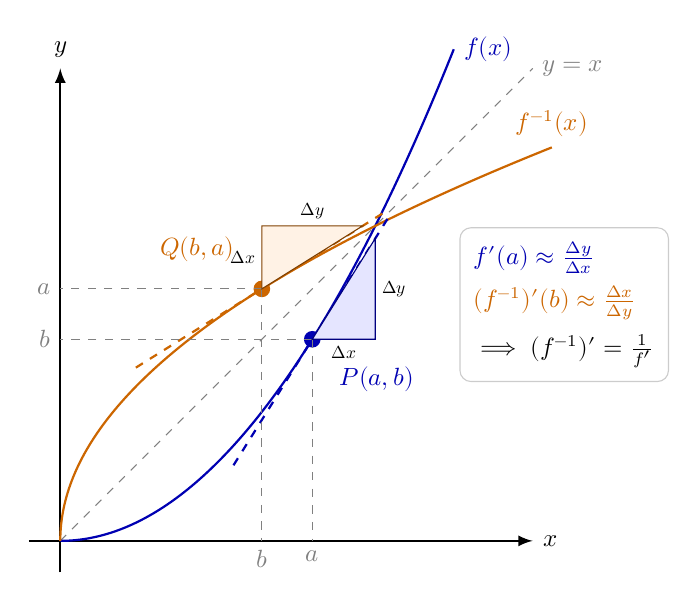
\begin{tikzpicture}[scale=2, >=latex, font=\small]
        % --- 定义样式 ---
        \tikzset{
            func/.style={thick, color=blue!70!black},
            invfunc/.style={thick, color=orange!80!black},
            tangent/.style={thick, dashed, color=gray},
            axis/.style={->, thick, color=black},
            mirror/.style={dashed, color=black!50},
            aux/.style={dashed, thin, color=gray}
        }

        % --- 参数设置 ---
        % 定义函数 f(x) = x^2 / 2
        % 选取点 x0 = 1.6
        \def\xZero{1.6}
        \def\yZero{1.28} % 1.6^2 / 2
        \def\slope{1.6}  % f'(x) = x -> f'(1.6) = 1.6
        
        % 计算反函数对应的点 (y0, x0)
        % 反函数斜率 = 1 / 1.6 = 0.625

        % --- 1. 绘制坐标系和对称轴 ---
        \draw[axis] (-0.2, 0) -- (3, 0) node[right] {$x$};
        \draw[axis] (0, -0.2) -- (0, 3) node[above] {$y$};
        \draw[mirror] (0, 0) -- (3, 3) node[right] {$y=x$};

        % --- 2. 绘制函数 f(x) ---
        \draw[func, domain=0:2.5, samples=100] plot (\x, {0.5*\x*\x}) node[right] {$f(x)$};

        % --- 3. 绘制反函数 f^{-1}(x) ---
        % 通过交换坐标绘制 (x, y) -> (y, x)
        \draw[invfunc, domain=0:2.5, samples=100] plot ({0.5*\x*\x}, \x) node[above] {$f^{-1}(x)$};

        % --- 4. 绘制点 P(a, b) 和切线 ---
        \coordinate (P) at (\xZero, \yZero);
        \fill[blue!70!black] (P) circle (1.5pt) node[below right=9pt] {$P(a, b)$};
        
        % 绘制切线 (长度适中)
        \draw[tangent, blue!70!black] 
            ($ (P) - (0.5, 0.5*\slope) $) -- ($ (P) + (0.5, 0.5*\slope) $);

        % --- 5. 绘制点 Q(b, a) 和切线 ---
        \coordinate (Q) at (\yZero, \xZero);
        \fill[orange!80!black] (Q) circle (1.5pt) node[above left=9pt] {$Q(b, a)$};
        
        % 反函数的切线 (斜率互为倒数)
        \draw[tangent, orange!80!black] 
            ($ (Q) - (0.5*\slope, 0.5) $) -- ($ (Q) + (0.5*\slope, 0.5) $);

        % --- 6. 辅助线 (坐标投影) ---
        \draw[aux] (P) -- (\xZero, 0) node[below] {$a$};
        \draw[aux] (P) -- (0, \yZero) node[left] {$b$};
        \draw[aux] (Q) -- (\yZero, 0) node[below] {$b$};
        \draw[aux] (Q) -- (0, \xZero) node[left] {$a$};

        % --- 7. 关键：斜率三角形 (Slope Triangles) ---
        
        % P点处的三角形 (dx, dy)
        \def\dt{0.4} % delta t (三角形大小)
        \coordinate (P_right) at (\xZero + \dt, \yZero);
        \coordinate (P_top) at (\xZero + \dt, \yZero + \slope*\dt);
        
        \draw[fill=blue!10, draw=blue!50!black] (P) -- (P_right) -- (P_top) -- cycle;
        \node[scale=0.7, below] at ($ (P)!0.5!(P_right) $) {$\Delta x$};
        \node[scale=0.7, right] at ($ (P_right)!0.5!(P_top) $) {$\Delta y$};
        
        % Q点处的三角形 (翻转：dx 变竖直, dy 变水平)
        % 注意：在反函数中，Run是原来的dy，Rise是原来的dx
        \coordinate (Q_top) at (\yZero, \xZero + \dt);
        \coordinate (Q_right) at (\yZero + \slope*\dt, \xZero + \dt);
        
        \draw[fill=orange!10, draw=orange!50!black] (Q) -- (Q_top) -- (Q_right) -- cycle;
        
        % 这里的标签非常关键：展示 dx 变成了 Rise
        \node[scale=0.7, left] at ($ (Q)!0.5!(Q_top) $) {$\Delta x$}; 
        \node[scale=0.7, above] at ($ (Q_top)!0.5!(Q_right) $) {$\Delta y$};

        % --- 8. 结论文字 ---
        \node[align=left, fill=white, draw=black!20, rounded corners, inner sep=5pt] at (3.2, 1.5) {
            \textcolor{blue!70!black}{$f'(a) \approx \frac{\Delta y}{\Delta x}$} \\[0.5em]
            \textcolor{orange!80!black}{$(f^{-1})'(b) \approx \frac{\Delta x}{\Delta y}$} \\[0.5em]
            $\implies (f^{-1})' = \frac{1}{f'}$
        };

    \end{tikzpicture}
    \end{figure}


    \begin{remark}
    函数 $y=f(x)$ 的图像关于直线 $y=x$ 对称后得到 $y=f^{-1}(x)$ 的图像。
    如果原函数在点 $(x_0, y_0)$ 处的切线斜率为 $m = f'(x_0)$（且 $m \neq 0$），
    那么其对称图像在对应点 $(y_0, x_0)$ 处的切线斜率就是 $1/m$。\\

    这也是为什么我们需要条件 $f'(x_0) \neq 0$，因为如果原函数切线水平，
    反函数在对应点的切线将是垂直的，斜率不存在（无穷大）。
    \end{remark}


    \section{Mean Value Theorem}

    \subsection{Fermat's Theorem}

    \begin{theorem}[Local Extreme Theorem / Fermat's Theorem]
    Let $f: (a, b) \to \mathbb{R}$ be differentiable. If $f$ attains a local maximum or minimum at $x_0 \in (a, b)$,
    then $$f'(x_0) = 0$$
    \end{theorem}

    \begin{analysis}
        Draw a sketch about a function:
        \begin{figure}[H]
            \centering
        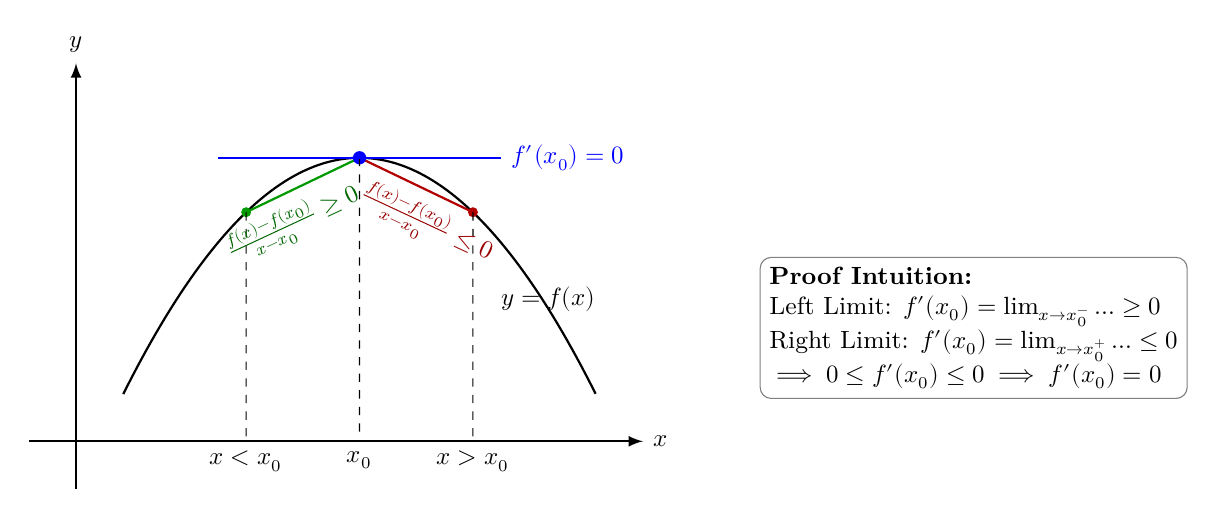
\begin{tikzpicture}[scale=1.2, >=latex, font=\small]

            % --- 1. 坐标系 ---
            \draw[->, thick] (-0.5, 0) -- (6, 0) node[right] {$x$};
            \draw[->, thick] (0, -0.5) -- (0, 4) node[above] {$y$};

            % --- 2. 定义函数曲线 (抛物线模拟局部最大值) ---
            % 顶点在 (3, 3) 用来表示局部最大值
            \draw[thick, domain=0.5:5.5, samples=100] plot (\x, {-0.4*(\x-3)^2 + 3});
            \node at (5, 1.5) {$y=f(x)$};

            % --- 3. 关键点设置 ---
            \coordinate (X0) at (3, 3);       % 极值点 x0
            \coordinate (XL) at (1.8, 2.424); % 左侧点 x0 - h
            \coordinate (XR) at (4.2, 2.424); % 右侧点 x0 + h

            % --- 4. 绘制左侧逼近 (上坡) ---
            % 绘制割线
            \draw[green!60!black, thick] (XL) -- (X0);
            % 标注点
            \fill[green!60!black] (XL) circle (1.5pt);
            \draw[dashed] (XL) -- (1.8, 0) node[below] {$x < x_0$};
            % 斜率说明
            \node[green!40!black, rotate=25] at (2.3, 2.3) {$\frac{f(x)-f(x_0)}{x-x_0} \ge 0$};

            % --- 5. 绘制右侧逼近 (下坡) ---
            % 绘制割线
            \draw[red!70!black, thick] (X0) -- (XR);
            % 标注点
            \fill[red!70!black] (XR) circle (1.5pt);
            \draw[dashed] (XR) -- (4.2, 0) node[below] {$x > x_0$};
            % 斜率说明
            \node[red!60!black, rotate=-25] at (3.7, 2.3) {$\frac{f(x)-f(x_0)}{x-x_0} \le 0$};

            % --- 6. 绘制极值点和切线 ---
            \fill[blue] (X0) circle (2pt);
            \draw[dashed] (X0) -- (3, 0) node[below] {$x_0$};
            
            % 水平切线
            \draw[blue, thick] (1.5, 3) -- (4.5, 3) node[right] {$f'(x_0) = 0$};

            % --- 7. 逻辑推导框 ---
            \node[align=left, fill=white, draw=gray, rounded corners] at (9.5, 1.2) {
                \textbf{Proof Intuition:} \\
                Left Limit: $f'(x_0) = \lim_{x \to x_0^-} \dots \ge 0$ \\
                Right Limit: $f'(x_0) = \lim_{x \to x_0^+} \dots \le 0$ \\
                $\implies 0 \le f'(x_0) \le 0 \implies f'(x_0) = 0$
            };
        \end{tikzpicture}
        \end{figure}
    \end{analysis}

    \begin{proof}
    Assume $f(x_0) = \min_{x \in (a, b)} f(x)$. Then for any $x$, $f(x) \ge f(x_0)$.
    Considering the one-sided limits:
    \begin{enumerate}
        \item As $x \to x_0^+$, $x - x_0 > 0 \implies \frac{f(x) - f(x_0)}{x - x_0} \ge 0 \implies f'(x_0) \ge 0$
        \item As $x \to x_0^-$, $x - x_0 < 0 \implies \frac{f(x) - f(x_0)}{x - x_0} \le 0 \implies f'(x_0) \le 0$
    \end{enumerate}
    Since $f$ is differentiable, the limit exists, so we must have $f'(x_0) = 0$.\\

    The proof for a local maximum is similar.
    \end{proof}

    \begin{remark}
        定理成立的前提是函数在极值点 $x_0$ 处必须可导。
        若函数在极值点处形成“尖点”（Cusp）或“角点”（Corner），导数不存在，则无法得出导数为 0 的结论。
    \end{remark}

    \begin{remark}
        导数为 $0$ 只是极值存在的必要条件，而非充分条件。
    \end{remark}

    \newpage

    \subsection{Mean Value Theorem}

    \begin{lemma}[Rolle's Theorem]
    Let $f$ be continuous on $[a, b]$ and differentiable on $(a, b)$. If $f(a) = f(b)$, then:
    \[ \exists z_0 \in (a, b)\ \text{ s.t }\ f'(z_0) = 0 \]
    \end{lemma}

    \begin{proof}
    If $f$ is constant, $f'(x) = 0$ everywhere, and the theorem holds trivially.\\

    Assume $f$ is not constant. By the \textbf{Extreme Value Theorem}, 
    $f$ attains a maximum $M$ and a minimum $m$ on $[a, b]$.\\

    Since $f$ is not constant and $f(a) = f(b)$, 
    at least one of the extremum points must lie in the open interval $(a, b)$.
    Let $z_0 \in (a, b)$ be such an extreme point. By the Local Extreme Theorem, $f'(z_0) = 0$.
    \end{proof}

    \begin{remark}
        连续性条件至关重要。例如函数
        \[ f(x) = \begin{cases} 2x - 1 & x \in (1, 2] \\ 3 & x = 1 \end{cases} \]
        虽然满足 $f(1)=f(2)=3$，但由于 $f$ 在 $x=1$ 处不连续，且在 $(1,2)$ 内 $f'(x)=2 \neq 0$，因此结论不成立。
    \end{remark}

    \begin{theorem}[Mean Value Theorem]
    Let $f$ be continuous on $[a, b]$ and differentiable on $(a, b)$. Then:
    \[ \exists x_0 \in (a, b) \text{ such that } f(b) - f(a) = f'(x_0)(b - a) \]
    \end{theorem}

    \begin{proof}
    We construct an function $F(x)$ representing the vertical distance between the curve $f(x)$ and the secant line connecting $(a, f(a))$ and $(b, f(b))$:
    \[ F(x) = f(x) - \left[ \frac{f(b) - f(a)}{b - a}(x - a) + f(a) \right]. \]
    Observe that:
    \begin{enumerate}
        \item $F$ is continuous on $[a, b]$ and differentiable on $(a, b)$.
        \item $F(a) = f(a) - f(a) = 0$ and $F(b) = f(b) - f(b) = 0$.
    \end{enumerate}
    By Rolle's Theorem, $\exists x_0 \in (a, b)$ such that $F'(x_0) = 0$.
    Differentiating $F(x)$:
    \[ F'(x) = f'(x) - \frac{f(b) - f(a)}{b - a}. \]
    Setting $F'(x_0) = 0$ yields $f'(x_0) = \dfrac{f(b) - f(a)}{b - a}$.
    \end{proof}

    \begin{remark}
        罗尔定理实际上是 MVT 在 $f(a)=f(b)$ 时的特例。
    \end{remark}

    \newpage

    \begin{example}[Inequalities and Approximations]\quad
    \begin{enumerate}
        \item \textbf{Trigonometric Inequality}: For any $a, b \in \mathbb{R}$ with $a < b$, 
        prove $|\sin b - \sin a| \le |b - a|$.
        \begin{proof}
            Let $f(x) = \sin x$. By MVT on $[a, b]$, $\exists c \in (a, b)$ such that:
            \[ \frac{\sin b - \sin a}{b - a} = \cos c \]
            Since $|\cos c| \le 1$, 
            we have $\left|\dfrac{\sin b - \sin a}{b - a}\right| \le 1 \implies |\sin b - \sin a| \le |b - a|$.
        \end{proof}
        
        % \item \textbf{Approximation}: Estimate $\sqrt{16.1}$.
        % Let $f(x) = \sqrt{x}$. Apply MVT on $[16, 16.1]$. $\exists c \in (16, 16.1)$ such that:
        % \[ f(16.1) - f(16) = f'(c)(16.1 - 16) = \frac{1}{2\sqrt{c}} \cdot (0.1). \]
        % Approximating $c \approx 16$, we get $\frac{1}{2\sqrt{16}} = \frac{1}{8} = 0.125$.
        % \[ \sqrt{16.1} \approx 4 + 0.125 \times 0.1 = 4.0125. \]
        
        \item \textbf{Bernoulli's Inequality}: Prove that
        $$
        \text{$(1+x)^\alpha \ge 1 + \alpha x$ for $x > -1, \alpha \ge 1$}
        $$
        \begin{proof}
            Let $g(t) = (1+t)^\alpha - (1+\alpha t)$. Note $g(0) = 0$. We have
            $$g'(t) = \alpha(1+t)^{\alpha-1} - \alpha = \alpha[(1+t)^{\alpha-1} - 1]$$ 
            \begin{enumerate}
                \item For $x > 0$: Apply MVT on $[0, x]$. $\exists c \in (0, x)$ such that
                $$g(x) - g(0) = g'(c)(x - 0)$$
                Since $g'(c) = \alpha[(1+c)^{\alpha-1} - 1]$, 
                and $c > 0, \alpha \ge 1$, we have $g'(c) > 0$. Thus $g(x) > 0$.

                \item For $-1 < x < 0$: Apply MVT on $[x, 0]$. $\exists c \in (x, 0)$ such that 
                $$g(0) - g(x) = g'(c)(0 - x)$$
                Here $c < 0$, so $(1+c)^{\alpha-1} < 1 \implies g'(c) < 0$. 
                Since $-x > 0$, the product is negative, implying $g(0) - g(x) < 0 \implies g(x) > 0$.
            \end{enumerate}
        \end{proof}
    \end{enumerate}
    \end{example}

    \newpage

    \subsection{Monotonicity of Functions}

    The MVT allows us to determine the global behavior of a function from the sign of its derivative.

    \begin{theorem}[Curve Tracing / Monotonicity Theorem]
    Let $f$ be differentiable on $(a, b)$.

    In \textbf{monotone} cases:
    \begin{enumerate}
        \item $f'(x) \ge 0, \forall x \in (a, b) \iff f$ is increasing on $(a, b)$.
        \item $f'(x) \le 0, \forall x \in (a, b) \iff f$ is decreasing on $(a, b)$.
        \item $f'(x) \equiv 0, \forall x \in (a, b) \iff f$ is constant on $(a, b)$.
    \end{enumerate}

    In \textbf{strictly monotone} cases:
    \begin{enumerate}
        \item $f'(x) > 0, \forall x \in (a, b) \implies f$ is strictly increasing on $(a, b)$.
        \item $f'(x) < 0, \forall x \in (a, b) \implies f$ is strictly decreasing on $(a, b)$.
    \end{enumerate}
    \end{theorem}

    \begin{proof}
    Let $x, y \in (a, b)$ with $x < y$. By MVT, there exists $c \in (x, y)$ such that:
    \begin{equation}\label{5.1}
        f(y) - f(x) = f'(c)(y - x)
    \end{equation}
    Since $y - x > 0$, the sign of $f(y) - f(x)$ is entirely determined by the sign of $f'(c)$.\\

    \textbf{Monotone cases:} ($\Rightarrow$) Since $y-x > 0$, by (\ref{5.1}) we have
    \begin{center}
            $
    \begin{cases}
        f(y) - f(x) \geq 0 & \text{if $f'(x) \ge 0$} \\[1ex]
        f(y) - f(x) \leq 0 & \text{if $f'(x) \le 0$} \\[1ex]
        f(y) - f(x) = 0 & \text{if $f'(x) = 0$}
    \end{cases}
    $
    \end{center}

    \textbf{Monotone cases:} ($\Leftarrow$) If $f$ monotonic, then
    \begin{center}
    $
    \begin{cases}
        \dfrac{f(x) - f(x_0)}{x-x_0} \geq 0 \implies \displaystyle\lim_{x \to x_0} \dfrac{f(x) - f(x_0)}{x-x_0} \geq 0 & \text{if $x > x_0 \implies f(x) \geq f(x_0)$}  \\[2ex]
        \dfrac{f(x) - f(x_0)}{x-x_0} \leq 0 \implies \displaystyle\lim_{x \to x_0} \dfrac{f(x) - f(x_0)}{x-x_0} \leq 0 &  \text{if $x > x_0 \implies f(x) \leq f(x_0)$}  \\[2ex]
        \dfrac{f(x) - f(x_0)}{x-x_0} = 0 \implies \displaystyle\lim_{x \to x_0} \dfrac{f(x) - f(x_0)}{x-x_0} = 0 & \text{if $\forall x_0 \in (a,b),\ f(x) = f(x_0)$}
    \end{cases}
    $
    \end{center}

    \textbf{Strictly monotone cases:} Since $y-x > 0$, by (\ref{5.1}) we have
    \begin{center}
    $
    \begin{cases}
        f(y) - f(x) > 0 & \text{if $f'(x) > 0$} \\
        f(y) - f(x) < 0 & \text{if $f'(x) < 0$} 
    \end{cases}
    $
    \end{center}
    \end{proof}

    \begin{remark}
    \begin{enumerate}
        \item 结合 $f' > 0$ 意味着严格单调递增，我们可以进而推断出该函数是单射。
        \item $f' \equiv 0 \implies f$ 是常数，
        这在证明两个函数恒等时非常有用（即只需证明它们的导数相等且在某一点值相等）。
    \end{enumerate}
    \end{remark}

    \newpage
    
    \begin{remark}
    \textbf{单调性定理的逆命题}：
        对于可微函数 $f$，如果 $f$ 在 $(a,b)$ 是严格递增、严格递减（单射的），
        我们不能推出 $f'(x) \neq 0$ 在所有点成立（即不能保证 $f'(x) > 0$ 或 $f'(x) < 0$ 恒成立）。
        \begin{itemize}
            \item \textbf{反例}：考虑函数 $f: \mathbb{R} \to \mathbb{R}$，定义为 $f(x) = x^3$。
            \[ x_1 < x_2 \implies x_1^3 < x_2^3 \]
            该函数在 $\mathbb{R}$ 上是严格递增的，但在 $x=0$ 处，其导数 $f'(0) = 0$。
        \end{itemize}
    \end{remark}

    \begin{theorem}[Local Tracing Theorem / 局部保号定理]
    Let $f: [a, b] \to \mathbb{R}$ be continuous and differentiable at $c \in [a, b]$. 
    If $f'(c) > 0$, then there exist $c_0, c_1 \in \mathbb{R}$ with $c_0 < c < c_1$ such that:
    \begin{align*}
        x \in (c_0, c) \cap [a, b] &\implies f(x) < f(c), \\
        y \in (c, c_1) \cap [a, b] &\implies f(y) > f(c).
    \end{align*}
    Similarly, if $f'(c) < 0$, the inequalities are reversed ($f(x) > f(c) > f(y)$ locally).
    \end{theorem}

    \begin{proof}
    Let $f'(c) > 0$. We prove the existence of the left neighborhood $(c_0, c)$ by contradiction.
    Assume there is no such $c_0$. Then for any $n \in \mathbb{N}$, there exists a point $x_n$ in the interval $(c - \frac{1}{n}, c) \cap [a, b]$ such that the condition fails, i.e.,
    \[ f(x_n) \ge f(c). \]
    This implies the difference quotient is non-positive:
    \[ \frac{f(x_n) - f(c)}{x_n - c} \le 0 \quad (\text{Since } f(x_n) - f(c) \ge 0 \text{ and } x_n - c < 0). \]
    Since $x_n \in (c - 1/n, c)$, we have $x_n \to c$ as $n \to \infty$. By the definition of the derivative and the sequential limit theorem:
    \[ f'(c) = \lim_{n \to \infty} \frac{f(x_n) - f(c)}{x_n - c} \le 0. \]
    This contradicts the hypothesis that $f'(c) > 0$. Therefore, such a $c_0$ must exist.
    The proof for the existence of $c_1$ (right neighborhood) is similar.
    \end{proof}

    \begin{remark}
    需要注意的是，Local Tracing Theorem 并不等同于说
    “如果 $f'(c) > 0$，那么函数在 $c$ 的某个邻域内是单调递增的”。
    它只保证了：在 $c$ 左边的点比 $f(c)$ 小，在 $c$ 右边的点比 $f(c)$ 大。
    函数在这些邻域内部仍然可能是振荡的（即非单调的）。
    例如 
    $$f(x) = x + 2x^2 \sin(1/x)$$ 
    在 $x=0$ 处 $f'(0)=1 > 0$，但在 0 的任意邻域内都不是单调函数。
    \end{remark}

    \newpage

    \subsection{Generalized Mean Value Theorem}

    The Generalized Mean Value Theorem is an extension of the standard MVT involving two functions.

    \begin{theorem}[Generalized Mean Value Theorem / Cauchy's MVT]
    Let $f, g$ be continuous on $[a, b]$ and differentiable on $(a, b)$. Then there exists $x_0 \in (a, b)$ such that
    \[ g'(x_0)(f(b) - f(a)) = f'(x_0)(g(b) - g(a)) \]
    \end{theorem}

    \begin{proof}[An imperfect proof]
    Suppose $g(b) \ne g(a)$. We construct an function:
    \[ F(x) = g(x) \dfrac{f(b)-f(a)}{g(b)-g(a)} - f(x) \]
    We have $F(a) = f(b) = \dfrac{f(b)g(a) - g(b)f(a)}{g(b) - g(a)}$ and $F$ is continuous 
    on $[a, b]$ and differentiable on $(a, b)$, by \textbf{Rolle's Theorem}, 
    there exists $x_0 \in (a, b)$ such that $F'(x_0) = 0$:
    $$
    \begin{aligned}
            &F'(x_0) = g'(x_0) \dfrac{f(b)-f(a)}{g(b)-g(a)} - f'(x_0) = 0 \\
    \implies &f'(x_0)(g(b) - g(a)) = g'(x_0)(f(b) - f(a))
    \end{aligned}
    $$
    \end{proof}

    \begin{proof}[Improved proof]
    We re-change the function $F(x)$:
    $$
    \begin{aligned}
            F(x) &= g(x) \dfrac{f(b)-f(a)}{g(b)-g(a)} - f(x)\\
            F(x)(g(b)-g(a)) &= g(x) (f(b)-f(a)) - f(x)(g(b)-g(a))
    \end{aligned}
    $$
    Let $L(x) = g(x) (f(b)-f(a)) - f(x)(g(b)-g(a))$, 
    we have
    \begin{enumerate}
        \item $L(a) = L(b) = f(b)g(a) - g(b)f(a)$.
        \item $L$ is continuous on $[a, b]$ and differentiable on $(a, b)$.
    \end{enumerate}
    by \textbf{Rolle's Theorem}, 
    there exists $x_0 \in (a, b)$ such that $F'(x_0) = 0$:
    $$
    \begin{aligned}
            L(c) = 0 \implies g'(x_0)(f(b) - f(a)) = f'(x_0)(g(b) - g(a))
    \end{aligned}
    $$
    \end{proof}

    \begin{remark}
    \begin{enumerate}
        \item 如果令 $g(x) = x$，则 $g'(x) = 1$ 且 $g(b) - g(a) = b - a$。
        此时广义中值定理就退化为普通的拉格朗日中值定理。
        \item \textbf{几何意义}：如果 $g(b) \neq g(a)$ 且在区间内 $g'(x) \neq 0$，我们可以将定理写成比值的形式：
        \[ \frac{f(b) - f(a)}{g(b) - g(a)} = \frac{f'(x_0)}{g'(x_0)}. \]
        这表明：两个函数在区间上的总增量之比，等于它们在区间内某一点的瞬时变化率之比。
        这在参数方程求导和洛必达法则的证明中非常有用。
    \end{enumerate}
    \end{remark}

    \newpage

    \begin{example}
    Let $f: [1, 2] \to \mathbb{R}$ be continuous and differentiable on $(1, 2)$. Prove that there exists $\theta \in (1, 2)$ such that
    \[ f(2) - f(1) = \frac{1}{2}\theta^2 f'(\theta) \]
    \begin{proof}
            Rearranging the target equation to identify the structure of Cauchy's MVT:
    \[ \theta^2 f'(\theta) = \frac{f'(\theta)}{1/\theta^2} = \frac{f'(\theta)}{-\frac{d}{d\theta}(1/\theta)}. \]
    Let $g(x) = \frac{1}{x}$. Then $g'(x) = -\frac{1}{x^2}$.
    Applying the Generalized MVT to $f(x)$ and $g(x)$ on $[1, 2]$, there exists $\theta \in (1, 2)$ such that:
    \[ \frac{f(2) - f(1)}{g(2) - g(1)} = \frac{f'(\theta)}{g'(\theta)} \]
    Calculations:
    \begin{enumerate}
        \item LHS: $\frac{f(2) - f(1)}{\frac{1}{2} - 1} = \frac{f(2) - f(1)}{-1/2} = -2[f(2) - f(1)]$.
        \item RHS: $\frac{f'(\theta)}{-1/\theta^2} = -\theta^2 f'(\theta)$.
    \end{enumerate}
    \[ -2[f(2) - f(1)] = -\theta^2 f'(\theta) \implies f(2) - f(1) = \frac{1}{2}\theta^2 f'(\theta) \]

    \end{proof}
    \end{example}

    \begin{example}
    Suppose $0 < a < b$. Let $f: [a, b] \to \mathbb{R}$ be continuous and differentiable. Prove that there exists $\theta \in (a, b)$ such that
    \[ \frac{1}{b - a} \begin{vmatrix} f(a) & f(b) \\ a & b \end{vmatrix} = f(\theta) - \theta f'(\theta) \]
    \begin{proof}
        First, expand the determinant :
        \[ \text{LHS} = \frac{1}{b - a} [b f(a) - a f(b)] = \frac{b f(a) - a f(b)}{b - a} = \frac{\frac{f(a)}{a} - \frac{f(b)}{b}}{\frac{1}{a} - \frac{1}{b}} \]
        % To apply Cauchy's MVT, we try to rewrite this fraction as a difference quotient $\frac{F(b) - F(a)}{G(b) - G(a)}$.
        % Limit the numerator and denominator by dividing by $ab$:
        % \[ \frac{b f(a) - a f(b)}{b - a} = \frac{\frac{b f(a) - a f(b)}{ab}}{\frac{b - a}{ab}} = \frac{\frac{f(a)}{a} - \frac{f(b)}{b}}{\frac{1}{a} - \frac{1}{b}}. \]
        Defining two functions:
        \[ F(x) = \frac{f(x)}{x}, \quad G(x) = \frac{1}{x}. \]
        Apply Generalized MVT to $F$ and $G$ on $[a, b]$. There exists $\theta \in (a, b)$ such that:
        $$
        \begin{aligned}
            \frac{F(b) - F(a)}{G(b) - G(a)} &= \frac{F'(\theta)}{G'(\theta)} \\
            &= \frac{\frac{\theta f'(\theta) - f(\theta)}{\theta^2}}{-\frac{1}{\theta^2}} \\
            &= -(\theta f'(\theta) - f(\theta)) = f(\theta) - \theta f'(\theta)
        \end{aligned}
        $$
        % We already showed LHS is equal to the determinant expression. Now compute the derivatives:
        % \begin{itemize}
        %     \item $F'(\theta) = \frac{\theta f'(\theta) - f(\theta)}{\theta^2}$.
        %     \item $G'(\theta) = -\frac{1}{\theta^2}$.
        % \end{itemize}
        % Substituting into the ratio:
        % \[ \frac{F'(\theta)}{G'(\theta)} = \frac{\frac{\theta f'(\theta) - f(\theta)}{\theta^2}}{-\frac{1}{\theta^2}} = -(\theta f'(\theta) - f(\theta)) = f(\theta) - \theta f'(\theta) \]
        Thus, the equation holds.
    \end{proof}
    \end{example}
    
    \newpage

    \section{Taylor Series and Taylor Polynomial}

        
    \begin{theorem}[Taylor's Theorem]
    Let $f: (a, b) \to \mathbb{R}$ be $n$ times differentiable on $(a, b)$. 
    For every $x, c \in (a, b)$, there exists $x_0$ strictly between $x$ and $c$ such that:
    \[ f(x) = \sum_{k=0}^{n-1} \frac{f^{(k)}(c)}{k!} (x - c)^k + \frac{f^{(n)}(x_0)}{n!} (x - c)^n \]
    \end{theorem}

    \begin{remark}
    \textbf{关于公式结构的说明}：
    \begin{enumerate}
        \item 前面的求和部分 $\displaystyle\sum_{k=0}^{n-1} \frac{f^{(k)}(c)}{k!} (x - c)^k$ 
        称为 $f$ 在 $c$ 点的 \textbf{$(n-1)$ 阶泰勒多项式}。

        \item 最后一项 $R_n(x) = \dfrac{f^{(n)}(x_0)}{n!} (x - c)^n$ 
        称为 \textbf{拉格朗日余项 (Lagrange form of the remainder)}。它量化了多项式逼近的误差。
        
        \item 注意这里的 $n$ 阶可导通常意味着前 $n-1$ 阶导数连续，第 $n$ 阶导数存在。
    \end{enumerate}
    \end{remark}

    \begin{proof}
    Let $R_n(t)$ be the error function defined for any $t \in (a, b)$:
    \[ R_n(t) = f(t) - \sum_{k=0}^{n-1} \frac{f^{(k)}(c)}{k!} (t - c)^k. \]
    We aim to prove $R_n(x) = \dfrac{f^{(n)(x_0)}}{n!}(x-c)^n$.
    Let $g(t) = (t - c)^n$. 
    Note that $$g(c) = g'(c) =  \dots = g^{(n-1)}(c) = 0$$
    and $g^{(n)}(t) = n!$.
    Similarly, one can check that $$R_n(c) = R_n'(c) = \dots = R_n^{(n-1)}(c) = 0$$

    We apply the \textbf{Generalized Mean Value Theorem} repeatedly.
    \begin{enumerate}
        \item Apply Cauchy MVT to $R_n(t)$ and $g(t)$ on $[c, x]$. 
        There exists $\gamma_1$ between $x$ and $c$ such that:
        \[ \frac{R_n(x) - R_n(c)}{g(x) - g(c)} = \frac{R_n(x)}{(x-c)^n} = \frac{R_n'(\gamma_1)}{g'(\gamma_1)} = \frac{R_n'(\gamma_1)}{n(\gamma_1 - c)^{n-1}}. \]
        
        \item Apply Cauchy MVT to $R_n'(t)$ and $g'(t)$ on $[c, \gamma_1]$. There exists $\gamma_2$ between $\gamma_1$ and $c$ such that:
        \[ \frac{R_n'(\gamma_1) - R_n'(c)}{g'(\gamma_1) - g'(c)} = \frac{R_n'(\gamma_1)}{g'(\gamma_1)} = \frac{R_n''(\gamma_2)}{g''(\gamma_2)}. \]
        
        \item Repeating this process $n$ times, we find a sequence of points $\gamma_1, \gamma_2, \dots, \gamma_n$ (let $\gamma_n = x_0$) such that:
        \[ \frac{R_n(x)}{(x-c)^n} = \frac{R_n^{(n)}(x_0)}{g^{(n)}(x_0)}. \]
    \end{enumerate}
    Since $g^{(n)}(t) = n!$ and $R_n^{(n)}(t) = f^{(n)}(t)$ , we get:
    \[ \frac{R_n(x)}{(x-c)^n} = \frac{f^{(n)}(x_0)}{n!} \implies R_n(x) = \frac{f^{(n)}(x_0)}{n!} (x - c)^n. \]
    \end{proof}

    \newpage

    If a function is infinitely differentiable, we can consider the limit as $n \to \infty$.

    \begin{corollary}[Taylor Series]
    Let $f: (a, b) \to \mathbb{R}$ be infinitely differentiable. For $x \in (a, b)$, if $\lim_{n \to \infty} R_n(x) = 0$, then $f$ equals its Taylor series expansion:
    \[ f(x) = \sum_{n=0}^{\infty} \frac{f^{(n)}(c)}{n!} (x - c)^n. \]
    \end{corollary}

    Here are the Maclaurin series expansions (Taylor series at $c=0$) for some common elementary functions.

    \begin{example}\quad
    \begin{enumerate}
        \item \textbf{Exponential Function} ($e^x$):
        \[ e^x = \sum_{k=0}^n \frac{x^k}{k!} + R_{n+1}(x) = 1 + x + \frac{x^2}{2!} + \dots + \frac{x^n}{n!} + R_{n+1}(x). \]
        Since $R_n(x) \to 0$ for all $x$, $e^x = \sum_{n=0}^\infty \frac{x^n}{n!}$.

        \item \textbf{Trigonometric Functions}:
        \[ \cos x = \sum_{k=0}^n \frac{(-1)^k x^{2k}}{(2k)!} + R_{2n+2}(x) = 1 - \frac{x^2}{2!} + \frac{x^4}{4!} - \dots \]
        \[ \sin x = \sum_{k=0}^n \frac{(-1)^k x^{2k+1}}{(2k+1)!} + R_{2n+3}(x) = x - \frac{x^3}{3!} + \frac{x^5}{5!} - \dots \]
        
        \item \textbf{Logarithmic Function} ($\ln(1+x)$):
        \[ \ln(1+x) = \sum_{k=1}^n (-1)^{k-1} \frac{x^k}{k} + R_{n+1}(x) = x - \frac{x^2}{2} + \frac{x^3}{3} - \dots \]
        
        \item \textbf{Binomial Series} ($(1+x)^a$):
        \[ (1+x)^a = 1 + \sum_{k=1}^n \binom{a}{k} x^k + R_{n+1}(x) = 1 + ax + \frac{a(a-1)}{2!}x^2 + \dots \]
        where $\binom{a}{k} = \frac{a(a-1)\cdots(a-k+1)}{k!}$.

        \item \textbf{Inverse Trigonometric Functions}:
        \[ \arctan x = \sum_{k=0}^n \frac{(-1)^k x^{2k+1}}{2k+1} + R_{2n+3}(x) = x - \frac{x^3}{3} + \frac{x^5}{5} - \dots \]
        \[ \arcsin x = x + \sum_{k=1}^n \frac{(2k-1)!!}{(2k)!!} \frac{x^{2k+1}}{2k+1} + R_{2n+3}(x) \]
    \end{enumerate}
    \end{example}

    \newpage

    \chapter{Riemann-Stieltjes Integral}

    \section{Riemann-Stieltjes Integral}

    \subsection{Riemann-Stieltjes Sum}

    In this subsection we arrange $f: [a, b] \to \mathbb{R} $ be a bounded function and 
        $\alpha$ be a monotonically increasing function on $[a, b]$.

    \begin{definition}[Partition]
    A \textbf{partition} (分割) $P$ of $[a, b]$ is a finite set 
    of points $\{t_0, t_1, \dots, t_n\}$ such that:
    \[ a = t_0 < t_1 < \dots < t_n = b \]
    Denoted the set: $\mathcal{P}[a,b] = \{ P \mid \text{$P$ is a partition on $[a,b]$} \}$.
    \end{definition}

    \begin{definition}[Riemann-Stieltjes Sums / 黎曼-斯蒂尔杰斯和]
        Let $P = \{t_0, t_1, \dots, t_n\}$ be an partition on $[a,b]$. \\

        For each subinterval $[t_{j-1}, t_j]$ where $j = 1, \dots, n$, 
        we define the length $$\Delta \alpha_j = t_j - t_{j-1}$$ 
        and the Riemann-Stieltjes Sums as
        \[ S(f,P,\alpha) = \sum_{j=1}^{n} f(x_j)\Delta\alpha_j \quad (x_j \in [t_{j-1}, t_j] ) \\ \]
        Moreover, we define the extreme values:
        \[ M_j = \sup \{ f(x) \mid x \in [t_{j-1}, t_j] \}, \quad m_j = \inf \{ f(x) \mid x \in [t_{j-1}, t_j] \} \]
        Using these, we define the Lower / Upper Riemann-Stieltjes Sums:
        \begin{align*}
            L(f, P,\alpha) &= \sum_{j=1}^n m_j \Delta \alpha_j \\
            U(f, P,\alpha) &= \sum_{j=1}^n M_j \Delta \alpha_j
        \end{align*}
    \end{definition}

    \begin{remark}
        显然，对于任意分割 $P$，都有 $L(f, P,\alpha) \le S(f, P,\alpha) \le U(f, P,\alpha)$。
    \end{remark}

    \begin{remark}
        若 $\alpha(x) = x$，我们习惯写 $L(f, P) , U(f, P), S(f, P)$ 代替 $L(f, P,\alpha) , U(f, P,\alpha), S(f, P,\alpha)$。
        其对应的和也被称为上/下黎曼和。
    \end{remark}

    \begin{definition}[Refinement]
    Let $P$ and $P^*$ be two partitions of the interval $[a, b]$.
    \begin{enumerate}
        \item We say that $P^*$ is a \textbf{refinement} (加细) of $P$ if $P \subseteq P^*$. That is, every point in partition $P$ is also a point in partition $P^*$.
        \item Given two partitions $P_1$ and $P_2$, their \textbf{common refinement} is defined as the union of their points:
        \[ P^* = P_1 \cup P_2 \]
    \end{enumerate}
    \end{definition}

    \begin{theorem}[Refinement Theorem / 加细定理]
    If $P,Q \in \mathcal{P}[a,b]$ such that $P \subseteq Q$ (i.e., $Q$ is a \textbf{refinement} of $P$), then:
    \[ L(f, P, \alpha) \le L(f, Q, \alpha) \le U(f, Q, \alpha) \le U(f, P, \alpha) \]
    \end{theorem}

    \begin{proof}
    \textbf{Step 1: Single Point Addition} \\
    Suppose $P \subseteq Q$. Let $P = \{t_0, t_1, \dots, t_n\}$ and 
    let the extra point be $u$ such that $t_{k-1} < u < t_k$ for some $k$.
    Thus, $Q = \{t_0, \dots, t_{k-1}, u, t_k, \dots, t_n\}$.

    We have
    \begin{align*}
        m_k &= \inf \{ f(x) \mid x \in [t_{k-1}, t_k] \} = \min \{\inf_{ x \in [t_{k-1}, u ]}  f(x),  \inf_{ x \in [u , t_k]}  f(x) \}
    \end{align*}
    So
    $
    \begin{aligned}[t]
            L(f,P, \alpha) &= \sum_{j=1}^{n}m_k \Delta \alpha_j \leq L(f,P, \alpha) \\
                            &= \sum_{j=}^{k-1}m_j \Delta \alpha_j + m_k \Delta \alpha_k + \sum^{n}_{j=k+1}m_j \Delta \alpha_j \\
                            &\leq \sum_{j=1}^{k-1}m_j \Delta \alpha_j 
                            + \inf_{ x \in [t_{k-1}, u ]}  f(x) \Delta \alpha_k 
                            + \inf_{ x \in [u , t_k]}  f(x) \Delta \alpha_k 
                            + \sum^{n}_{j=k+1}m_j \Delta \alpha_j \\
                            &= L(f,Q, \alpha)
    \end{aligned}
    $\\

    \textbf{Step 2: General Case} \\
    Since $Q, P$ finite. Let $Q =P \cup \{u_i \mid i = 0,1,2,3,\cdots , r \}$. Use above result we have
    \[
    L(f, P,\alpha) \leq L(f, P \cup \{u_1\},\alpha) \leq L(f, P \cup \{u_1,u_2\},\alpha) \cdots \leq L(f, P \cup \{u_1,\cdots,u_r\},\alpha)= L(f, Q,\alpha)
    \]
    Similarly, we can show $U(f, P) \ge U(f, Q)$. Combined with the basic property $L(f, Q) \le U(f, Q)$, the full theorem is proved.
    \end{proof}

    % \begin{figure}[H]
    %     \centering
    %     \begin{tikzpicture}[scale=1.5]
    %         % Axis
    %         \draw[->] (0,0) -- (5,0) node[right] {$x$};
    %         \draw[->] (0,0) -- (0,3) node[above] {$y$};

    %         % Coordinates
    %         \def\tkprev{1}
    %         \def\u{2.5}
    %         \def\tk{4}
            
    %         % Function curve (concave up or wavy to show infimums)
    %         \def\curveFn{plot [smooth] coordinates {(1, 1.5) (1.8, 1.8) (2.5, 2.2) (3.2, 2.0) (4, 2.5)}}
    %         \draw[thick, blue] \curveFn node[above right] {$f(x)$};

    %         % m_k (Infimum over whole interval) is approx 1.5 at x=1
    %         \def\mk{1.5}
    %         \draw[dashed, red] (\tkprev, \mk) -- (\tk, \mk);
    %         \node[red, below] at (2.5, \mk) {\small $m_k$};
            
    %         % m' (Infimum over [tk-1, u]) approx 1.5
    %         \def\mprime{1.5}
            
    %         % m'' (Infimum over [u, tk]) approx 2.0 (at x=3.2)
    %         \def\mprimeprime{2.0}
            
    %         % Draw Rectangles for Split (Q)
    %         % Rect 1: [tk-1, u] height m'
    %         \draw[fill=green!20, opacity=0.6] (\tkprev, 0) rectangle (\u, \mprime);
    %         % Rect 2: [u, tk] height m''
    %         \draw[fill=green!40, opacity=0.6] (\u, 0) rectangle (\tk, \mprimeprime);

    %         % Draw Rectangle for Original (P) - Outline only
    %         \draw[thick, red] (\tkprev, 0) rectangle (\tk, \mk);

    %         % Labels
    %         \draw (\tkprev, 0.1) -- (\tkprev, -0.1) node[below] {$t_{k-1}$};
    %         \draw (\u, 0.1) -- (\u, -0.1) node[below] {$u$};
    %         \draw (\tk, 0.1) -- (\tk, -0.1) node[below] {$t_k$};

    %         \node at (1.75, 0.75) {$m'$};
    %         \node at (3.25, 1.0) {$m''$};
            
    %         \node[align=left, anchor=west] at (5.5, 1.5) {
    %             \textcolor{red}{\textbf{Original (P):}} Area $= m_k(t_k - t_{k-1})$ \\
    %             \textcolor{green!50!black}{\textbf{Refined (Q):}} Area $= m'(u - t_{k-1}) + m''(t_k - u)$ \\
    %             Since $m'' > m_k$, the green area $>$ red area.
    %         };
    %     \end{tikzpicture}
    %     \caption{Geometric Interpretation of Refinement. The area of the lower sum increases when a partition is refined.}
    % \end{figure}

    \begin{corollary}
        For any $P,Q \in \mathcal{P}[a,b]$ , we have:
        $$
            L(f,P,\alpha) \leq U(f,Q,\alpha) 
        $$
    \end{corollary}

    \begin{proof}
        Since $P,Q \subseteq P \cup Q$, we have
        $$L(f,P,\alpha) \leq L(f,P\cup Q,\alpha) \leq U(f,P\cup Q,\alpha) \leq U(f,Q,\alpha)$$
    \end{proof}

    \newpage

    \subsection{Riemann-Stieltje Integral}

    In this subsection we arrange $f: [a, b] \to \mathbb{R} $ be a bounded function and 
        $\alpha$ be a monotonically increasing function on $[a, b]$.

    \begin{definition}[Riemann-Stieltjes Integrable]
        For any $f$ on $[a,b]$, we said $f$ is integraable on $[a,b]$ iff for all  $\epsilon > 0$, 
        there exist $P_{\epsilon} \in \mathcal{P}[a,b]$ s.t $\forall P^{*} \supset P_{\epsilon}$ we have
        $$
            \left| S(f,P^{*},\alpha) - A \right| < \epsilon
        $$
        we said $f$ is \textbf{Riemann-Stieltjes Integraable} respect to $\alpha$, over $[a,b]$. Denote $A$ by 
        $$
            A  = \int_{a}^{b} f \diffd \alpha
        $$
        and the set $\mathcal{R}(\alpha)[a,b] = \{ f \mid \text{$f$ is Riemann-Stieltjes Integrable respect to $\alpha$, over $[a,b]$.} \}$.
    \end{definition}

    \begin{remark}
        It follows that $\inf (f) (b-a) \leq \int_{a}^{b} f \diffd \alpha < \sup (f) (b-a)$.
    \end{remark}

    \begin{definition}[Riemann-Stieltje Upper / Lower Integral]
    
        Let $L(f, P,\alpha), U(f, P,\alpha)$ be 
        lower / upper Riemann-Stieltjes Sum on $[a,b]$.
        Then define:
        $$
            \overline{\int}_{a}^{b}f(x) \diffd \alpha = \inf_P U(f, P,\alpha)
        $$
        is the Riemann-Stieltjes upper integral of $f$ with respect to $\alpha$, over $[a, b ]$, and
        $$
            \underline{\int}_{a}^{b}f(x) \diffd \alpha = \sup_P L(f, P,\alpha)
        $$
        is the Riemann-Stieltjes lower integral of $f$ with respect to $\alpha$, over $[a, b ]$.

    \end{definition}

    \begin{theorem}
        We have 
        $$
            \underline{\int}_{a}^{b}f(x) \diffd \alpha \leq \overline{\int}_{a}^{b}f(x) \diffd \alpha
        $$

    \end{theorem}

    \begin{proof}
        By Refinement Theorem, we have $\forall \epsilon >0 $, $\exists P \in \mathcal{P}[a,b]$ s.t.
        $$
        \underline{\int}_{a}^{b}f(x) \diffd \alpha - {\epsilon \over 2} < L(f , P, \alpha) \leq U(f , P, \alpha) <\overline{\int}_{a}^{b}f(x) \diffd \alpha  + {\epsilon \over 2}
        $$
        $\implies \overline{\int}_{a}^{b}f(x) \diffd \alpha - \underline{\int}_{a}^{b}f(x) \diffd \alpha < \epsilon \implies \underline{\int}_{a}^{b}f(x) \diffd \alpha \leq \overline{\int}_{a}^{b}f(x) \diffd \alpha$ 
        by finitesimal Principle (Theorem 2.1).
    \end{proof}

    \begin{remark}
        不等式
        $
        \underline{\int}_{a}^{b}f(x) \diffd \alpha - {\epsilon \over 2} < L(f , P, \alpha)
        $
        源自于上 / 下确界的性质，不要忘记上 / 下黎曼-斯蒂尔杰斯积分是集合的上 / 下确界。另一半不等式也同理。
    \end{remark}

    \newpage

    \subsection{Riemann Condition}

        In this subsection, we arrange $f: [a, b] \to \mathbb{R} $ be a bounded function,
        $\alpha$ be a monotonically increasing function on $[a, b]$ and $P=\{t_0,\cdots, t_n\}$ 
        be a partition of $[a,b]$.

    \begin{definition}[Riemann-Stieltje Condition]
    
        We said $f$ satisfied the Riemann-Stieltje Condition respect to $\alpha$ over $[a,b]$ iff 
        for all  $\epsilon > 0$, 
        there exist $P_{\epsilon} \in \mathcal{P}[a,b]$ s.t $\forall P^{*} \supset P_{\epsilon}$ we have
        $$
            U(f,P^{*},\alpha) - L(f,P^{*},\alpha) < \epsilon
        $$

    \end{definition}

    \begin{lemma}
        $f \in \mathcal{R}(\alpha)[a,b] \implies f$ satisfied the
        Riemann-Stieltje Condition respect to $\alpha$ over $[a,b]$.
    \end{lemma}

    \begin{analysis}
        $$
        \begin{aligned}[t]
            U(f,P^{*},\alpha) - L(f,P^{*},\alpha) &< \epsilon \\
            \iff \sum_{j=1}^{n}\left( M_j(f) - m_j(f) \right)\Delta \alpha_j &< \epsilon 
        \end{aligned}
        $$
        where $M_j(f) = \sup_{x \in [t_{j-1}, t_j]} f , m_j(f) = \inf_{x \in [t_{j-1}, t_j]} f$.
    \end{analysis}

    \begin{proof}
        $f \in \mathcal{R}(\alpha)[a,b] \implies $ for all  $\epsilon > 0$, 
        there exist $P_{\epsilon} \in \mathcal{P}[a,b]$ s.t $\forall P^{*} \supset P_{\epsilon}$ we have
        $$
        \begin{aligned}[t]
            \left| S(f,P^{*},\alpha) - \int_{a}^{b} f \diffd \alpha \right| &< \dfrac{\epsilon}{3} \\
            \left| \sum_{j=1}^{n}f(x_j)\Delta \alpha_j - \int_{a}^{b} f \diffd \alpha \right|&< \dfrac{\epsilon}{3} \quad (x_j \in [t_{j-1}, t_j]) 
        \end{aligned}
        $$
        for any $h > 0$ we have there are exist  $x_j,y_j \in [t_{j-1}, t_j]$ s.t.
        $$f(x_j) - f(y_j) > M_j (f) - m_j (f) - h$$
        \begin{remark}
            该不等式成立是因为
            $
            \begin{aligned}[t]
            M_j (f) - m_j (f) &= \sup_{x \in [t_{j-1}, t_j]} f - \inf_{x \in [t_{j-1}, t_j]} f \\
                            &= \sup_{x \in [t_{j-1}, t_j]} f + \sup_{x \in [t_{j-1}, t_j]} (-f) \\
                            &= \sup_{x, y \in [t_{j-1}, t_j]}( f(x) - f(y) )
            \end{aligned}
            $\\
            然后根据上确界的性质所得到。
        \end{remark}
        \noindent$\implies$
        $
        \begin{aligned}[t]
            \sum_{j=1}^{n}\left( M_j(f) - m_j(f) \right)\Delta \alpha_j  
            &< \sum_{j=1}^{n}\left( f(x_j) - f(y_j) +h \right)\Delta \alpha_j \\
            &<\sum_{j=1}^{n}\left( f(x_j) - f(y_j) \right)\Delta \alpha_j + \sum_{j=1}^{n} h \Delta \alpha_j \\
            &=\sum_{j=1}^{n} f(x_j) \Delta \alpha_j + \sum_{j=1}^{n} f(y_j) \Delta \alpha_j + h(\alpha(b) - \alpha(a))\\
            &< \dfrac{\epsilon}{3} + \dfrac{\epsilon}{3} + h(\alpha(b) - \alpha(a))
        \end{aligned}
        $\\

        Since $h>0$ is any number, take $h = \dfrac{\epsilon}{3(\alpha(b) - \alpha(a))}$, 
        we complete the proof.
        
    \end{proof}

    \newpage

    \newcommand{\lowerint}{\underline{\int}}
    \newcommand{\upperint}{\overline{\int}}

    \begin{lemma}
        $f$ satisfied the
        Riemann-Stieltje Condition respect to $\alpha$ over $[a,b] $ implies
        $$ \underline{\int}_{a}^{b}f(x) \diffd \alpha = \overline{\int}_{a}^{b}f(x) \diffd \alpha$$
    \end{lemma} 

    \begin{proof}
        By definition, for all  $\epsilon > 0$, 
        there exist $P_{\epsilon} \in \mathcal{P}[a,b]$ s.t $\forall P^{*} \supset P_{\epsilon}$ we have
        $$
            U(f,P^{*},\alpha) - L(f,P^{*},\alpha) < \epsilon
        $$
        By the inequality:
        $$
            L(f,P^*,\alpha) \leq \lowerint^{b}_a f(x) \diffd \alpha \leq \upperint^{b}_a f(x) \diffd \alpha \leq U(f,P^*,\alpha)
        $$
        we have
        $
        \begin{aligned}[t]
        &\upperint^{b}_a f(x) \diffd \alpha \leq U(f,P^*,\alpha) < L(f,P^*,\alpha) +\epsilon \leq \lowerint^{b}_a f(x) \diffd \alpha+\epsilon\\[1ex]
        \implies &\upperint^{b}_a f(x) \diffd \alpha < \lowerint^{b}_a f(x) \diffd \alpha + \epsilon
        \end{aligned}
        $\\

        By Infinitesimal Property we have 
        $\upperint^{b}_a f(x) \diffd \alpha \leq \lowerint^{b}_a f(x) \diffd \alpha + \epsilon$.
        Hence by Theorem 6.2 we have $\upperint^{b}_a f(x) \diffd \alpha = \lowerint^{b}_a f(x) \diffd \alpha$.
    \end{proof}

    \begin{lemma}
        $ \underline{\int}_{a}^{b}f(x) \diffd \alpha = \overline{\int}_{a}^{b}f(x) \diffd \alpha \implies f\in \mathcal{R}(\alpha)[a,b]$.
    \end{lemma}

    \begin{proof}
        
    \end{proof}

%----------------------------------------------------------------------------------------

\stopcontents[part] % Manually stop the 'part' table of contents here so the previous Part page table of contents doesn't list the following chapters

% \part{Part II: Real Analysis }

%----------------------------------------------------------------------------------------

\stopcontents[part]

%----------------------------------------------------------------------------------------
%	BIBLIOGRAPHY
%----------------------------------------------------------------------------------------

\chapterimage{} % Chapter heading image
\chapterspaceabove{2.5cm} % Whitespace from the top of the page to the chapter title on chapter pages
\chapterspacebelow{2cm} % Amount of vertical whitespace from the top margin to the start of the text on chapter pages

%------------------------------------------------

\chapter*{Bibliography}
\markboth{\sffamily\normalsize\bfseries Bibliography}{\sffamily\normalsize\bfseries Bibliography} % Set the page headers to display a Bibliography chapter name
\addcontentsline{toc}{chapter}{\textcolor{blue}{Bibliography}} % Add a Bibliography heading to the table of contents

\section*{Articles}
\addcontentsline{toc}{section}{Articles} % Add the Articles subheading to the table of contents

\printbibliography[heading=bibempty, type=article] % Output article bibliography entries

\section*{Books}
\addcontentsline{toc}{section}{Books} % Add the Books subheading to the table of contents

\printbibliography[heading=bibempty, type=book] % Output book bibliography entries

%----------------------------------------------------------------------------------------
%	INDEX
%----------------------------------------------------------------------------------------

\cleardoublepage % Make sure the index starts on an odd (right side) page
\phantomsection
\addcontentsline{toc}{chapter}{\textcolor{blue}{Index}} % Add an Index heading to the table of contents
\printindex % Output the index

%----------------------------------------------------------------------------------------
%	APPENDICES
%----------------------------------------------------------------------------------------

\chapterimage{orange2.jpg} % Chapter heading image
\chapterspaceabove{6.75cm} % Whitespace from the top of the page to the chapter title on chapter pages
\chapterspacebelow{7.25cm} % Amount of vertical whitespace from the top margin to the start of the text on chapter pages

\begin{appendices}

\renewcommand{\chaptername}{Appendix} % Change the chapter name to Appendix, i.e. "Appendix A: Title", instead of "Chapter A: Title" in the headers

%------------------------------------------------

\chapter{Appendix Chapter Title}

\section{Appendix Section Title}

Lorem ipsum dolor sit amet, consectetur adipiscing elit. Aliquam auctor mi risus, quis tempor libero hendrerit at. Duis hendrerit placerat quam et semper. Nam ultricies metus vehicula arcu viverra, vel ullamcorper justo elementum. Pellentesque vel mi ac lectus cursus posuere et nec ex. Fusce quis mauris egestas lacus commodo venenatis. Ut at arcu lectus. Donec et urna nunc. Morbi eu nisl cursus sapien eleifend tincidunt quis quis est. Donec ut orci ex. Praesent ligula enim, ullamcorper non lorem a, ultrices volutpat dolor. Nullam at imperdiet urna. Pellentesque nec velit eget est euismod pretium.

%------------------------------------------------

\chapter{Appendix Chapter Title}

\section{Appendix Section Title}

Lorem ipsum dolor sit amet, consectetur adipiscing elit. Aliquam auctor mi risus, quis tempor libero hendrerit at. Duis hendrerit placerat quam et semper. Nam ultricies metus vehicula arcu viverra, vel ullamcorper justo elementum. Pellentesque vel mi ac lectus cursus posuere et nec ex. Fusce quis mauris egestas lacus commodo venenatis. Ut at arcu lectus. Donec et urna nunc. Morbi eu nisl cursus sapien eleifend tincidunt quis quis est. Donec ut orci ex. Praesent ligula enim, ullamcorper non lorem a, ultrices volutpat dolor. Nullam at imperdiet urna. Pellentesque nec velit eget est euismod pretium.

%------------------------------------------------

\end{appendices}

%----------------------------------------------------------------------------------------

\end{document}
